% !TEX root = ../thesis_main.tex



%%%% --- * --- %%%%	
\clearpage
\chapter*{Long Comments}
\section{Round 0 and Earlier}
\addcontentsline{toc}{chapter}{Long Comments}

\note[tag]{Do everything in the giant list of giant-comments.}

\note[gg, nolist]{From Gerald:
\\...\\
Hi Melissa,
\\...\\
Attached is the report by Georg. I contains many valid points, and even for those where I'm not fully on board, it's clear that this has to be addressed. To be clear: This is not really that big of a deal. The actual work is not questioned in any way, and that's of course the really relevant part in the end. But it does have to be framed within a context, especially for the non-experts. I should have probably called off things like the handwritten appendix earlier, but thought that the committee members would ask for that in passing (on the basis that everything in the thesis must stand on its own, which those personal notes arguably don't; if this is relevant, it should be typed up).
\\...\\
I will write to the other committee members and call off their effort on this version, because Georg already won't sign off on it, so there is not point for them to go through it, as they most likely will agree with his points.
\\...\\
The course of action will now be for you to address these issues and then we'll resubmit.
\\...
}
\note[gg, nolist]{
...\\
I'm not entirely sold myself on a full "Standard Model intro" in the sense that the beta decay work stands on its own, and can be told as its own story. This is reflected by the fact that JTW predates the SM is is still fully relevant. So I'd go a somewhat light SM exposure. The most important goal is to make the non-experts comfortable in introducing what this is all about.
\\...\\
This will also bolster the citation count, which indeed looks suspiciously low (even though i'm not keen on such bean counting arguments).
\\...\\
Gerald
}

%%%%%%%%%%%%%%%%%%%%%%%%%%%
\note[done, nolist]{John's suggestions for fixing the stuff that Georg wanted fixed -- that giant email.  Moved to somewhere in Chapter~\ref{intro_chapter}.
\\...\\
hi Melissa,
\\
Gerald will soon send good clear corrections from a committee member. It will be clear you need to address those, and it will be clear what to do.
\\
Please read those first, and start answering them. Maybe then (and only then!) you will find two suggestions useful:
}
\note[moved, nolist]{From John, moved to the beginning of Ch.~\ref{intro_chapter}
\\
i) Among the necessary technical corrections, there's a solid request for more background info. I think you know what to do.
\\...\\
A large thing is some kind of extra qualitative description of what the SM is. You could do that qualitatively without any trouble.
\\...\\
You might point out some part of this:
\begin{itemize}
	\item the charged weak interaction you're writing down predates the Weinberg-Salam model by more than a decade. The version you've written down assumes protons and neutrons are fundamental particles.
	\item The exchange boson is much heavier in mass than the energy and momentum in the decay, so it can be approximated by an interaction with zero range. 
	\begin{itemize}
		\item Fermi did that very early on, 
		\item and Gamow and Teller added a process that change the nucleon spin. 
		\item Lee and Yang, which you cite, added the possible currents with different Lorentz transformations (do you mention that since any further combination of Dirac matrices can be reduced to these, so they span the space), and the possibility of parity violation by writing out helicity projections for the leptons. I.e. Lee and Yang assumed some fields (the nucleons and leptons) and a general interaction preserving the symmetries of the theory, which by definition is then an effective field theory.
	\end{itemize}
	\item Feynman and Gell-Mann's 1958 paper is the one that postulated V-A, again a decade before Weinberg-Salam, and they did this by making analogies between the boson exchanged and the photon, i.e. an analogy between the charged weak interaction and the electromagnetic current, so you could cite them instead of saying "SM predicts everything"
\end{itemize}
People had assumed there was a massive boson exchanged for a very long time.
\\
What Weinberg (and, independently, Salam) did was come up with a consistent mathematical theory of massive bosons, incorporating Yang Mills gauge theory (looks like E\&M but with nonabelian operators) to do that, and the result was the weak neutral interaction prediction.
}

\note[moved, nolist]{
ii) Similarly, answering how the results fit into the bigger picture is what you wanted to do.
\\...\\
I'm convinced that you don't want to do a full review of all beta decay experiments.
\\...\\
But you could say the Fierz term has been constrained by the energy spectrum and by the energy dependence of the beta
asymmetry, cite the best paper in the neutron and maybe the UCNA one as well, and use that figure I sent (I'm sending the improved version).
\\...\\
It is a good approximation to linearize the situation, i.e. this figure is good for small Cs and Ct. (A similar approach is being used in a letter coming out soon, and 3 referees did not nag them about it.)
}
%%%\begin{figure}[htb]
%%%	\centering
%%%	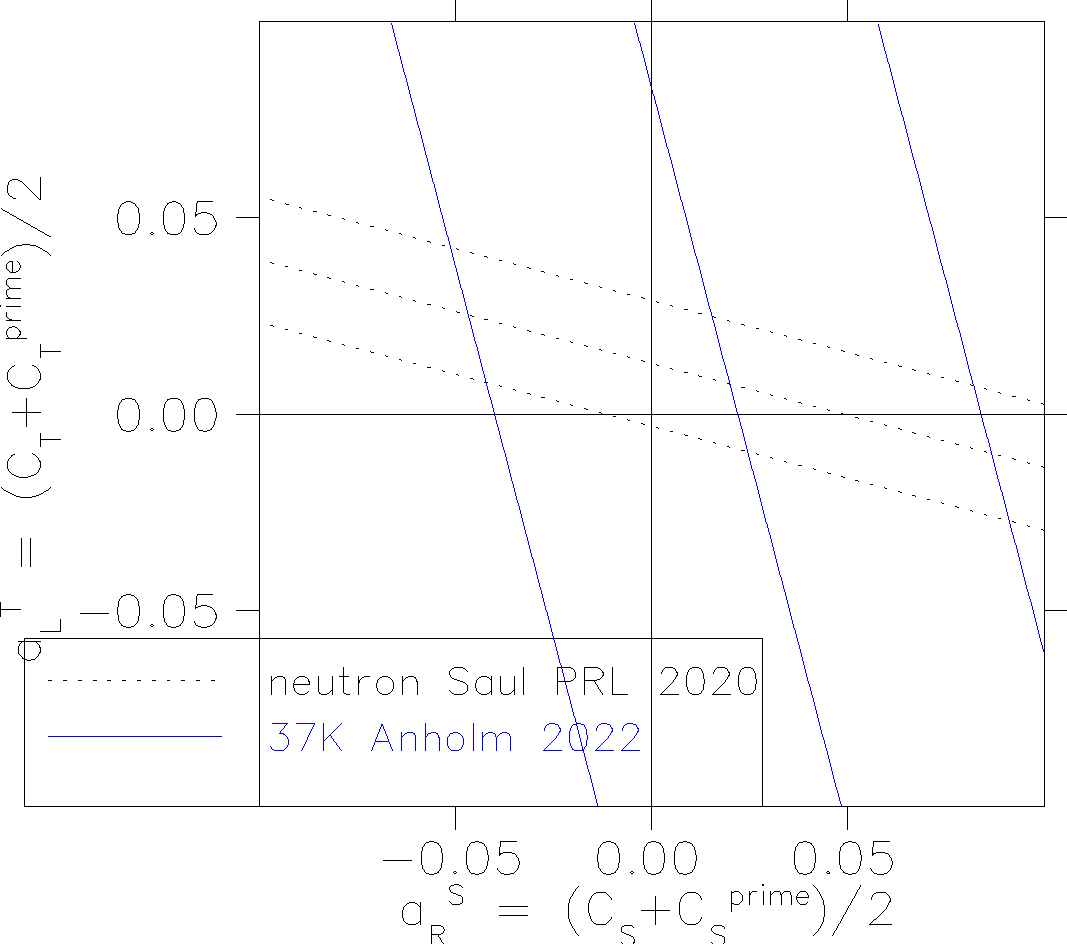
\includegraphics[width=.999\linewidth]{Figures/JB_exclusion.pdf}
%%%	\caption[That exclusion plot from John.]{That exclusion plot from John.  I think he means ``$C_S - C_S^\prime$'', etc.}	
%%%	\label{fig:nuclearleveldiagram_new}
%%%\end{figure}
That one figure with the $C_S$, $C_T$ used to be here.  But it's gone now.

\note[moved, nolist]{Immediate follow-up email from John:  
\\...\\
another basic big point. What would it mean if there were nonzero Cs, Ct? 
\\
In the context of the more elegant SM, a theory of quarks and leptons and mathematically consistent interactions, that would imply the existence of at least one extra unknown exchange boson. The mass would not be measured, just its coupling
strenghts to the particles participating in the beta decay.
\\...\\
Maybe background to understand that includes:
\\
If one were to write the SM weak interaction, $C_A$ and $C_V$ and $C_A$ and $C_V g_A$ would all be constants with abs value 1.
The (1+- gamma\_5)'s are projection operators-- in the SM, the W boson only couples to left-handed nu's and right-handed antinu's
\\
('more will be said in the forward-looking Ch. 6.2 about tests of that part.)
\\
So all the known information about Ca and Cv is accounted for.
\\
($g_A = 1.26$ for the neutron... it's not equal to 1 because of strong interactions between the quarks in the neutron.)
}

%%%%%%%%%%%%%%%%%%%%%%%%%%%
\FloatBarrier
\note[gs, nolist]{From Georg Schreckenbach:
\\
Re: Melissa Anholm, Ph.D. thesis, version April 18, 2022
\\
In response to your request for pre-evaluation of Melissa Anholm’s Ph.D. thesis, dated April 18, 2022, I believe that the thesis in its current form is \emph{not} ready for distribution.
}
\note[gs, nolist]
{
In my view, the following are critical problems:
\begin{enumerate}
    \item 1. The thesis in its current form is completely missing any embedding into a “bigger picture”.
    This would be the task of the Introduction chapter primarily, but should also significantly permeate other parts such as, notably, the conclusions. One could phrase this in the form of questions, including – but certainly not limited to – the following:
    \begin{itemize}
        \item - What is the Standard Model?
        \item - Why are we even searching for “physics beyond the standard model”? Why is there a need or desire to do so?
        \item - What other efforts have been or are being made to search for physics beyond the standard model? Have any of them been successful? If so – or if not, what does this mean?
        \item - Closely related to the previous question, how does the current work fit into this overall effort? What is the unique contribution here?
	\end{itemize}
    Etc.
%%%\end{enumerate}
%%%...\\
%%%}
%%%\note[gs, nolist]{
%%%\\...\\
%%%\begin{enumerate}
%%%	\setcounter{enumi}{1}
    \item 2. These aspects should be picked up in the Conclusions. What do the results mean for the “big
    picture”? Again, how do the fit in with the other efforts, prior, concurrent, or planned? Etc.
\end{enumerate}
}
\note[moved, nolist]{
\begin{enumerate}    
	\setcounter{enumi}{2}
    \item 3. As an outsider, it is my understanding that the author worked as part of a larger collaboration.
    It would be beneficial to clearly lay out what her unique contributions are. This could be
    done, for instance, in the Introduction, and/or the Conclusions.
\end{enumerate}
}
\note[gs, nolist]{
\begin{enumerate}    
	\setcounter{enumi}{3}
    \item 4. Formulas and symbols contained in these need to be defined, as do symbols that appear in the
    text. Currently, this is only done partly. It starts right at the beginning with Eq.~\ref{eq:betaplus_decay} (formerly 1.1) and continues throughout. Sure, one can of course guess the meaning of the symbols in Eq.~\ref{eq:betaplus_decay} – but one should not have to guess! – and this is certainly not true for later equations. (For instance, I have no idea about the meaning of most of the symbols in Eq.~\ref{equation:integrated_jtw_INTRODUCTION} (formerly 1.9), to give but one example.)
\end{enumerate}
}
\note[gs, nolist]{
\begin{enumerate}    
	\setcounter{enumi}{4}
    \item 5. Similarly, several figures need better explanations, starting with Fig. 1.1. Which, btw., also needs a source attribution (unless it was created by the author) and, presumably, a copyright note. Similar comments apply to various other figures as well.
\end{enumerate}
}
\note[moved, nolist]{
\begin{enumerate}    
	\setcounter{enumi}{5}
    \item 6. At first glance, I find a bibliography that contains only 28 entries to be problematic for a Ph.D. thesis. This goes, to some degree, back to my earlier points about embedding the work in the “bigger picture” – doing so would necessarily lead to several additional references – but it might be more than that.
\end{enumerate}
}
\note[done, nolist]{
\begin{enumerate}    
	\setcounter{enumi}{6}
    \item 7. Appendix C, adding scanned pictures of handwritten notes as figures that, moreover, seem not to be referenced at all, is – well – problematic. I don’t think that it conforms to the instructions as per Supplemental Regulations either (though I did not explicitly check).
\end{enumerate}
}
\note[gs, nolist]{
\\...\\
Given these various issues, I have not fully read the thesis in detail; I have instead focused on the question at hand: what is needed for the thesis to be in a form that can be distributed? I will provide a more formal report on the version of the thesis that I will receive from FGS.
\\...\\
Besides, there are some additional points that I would suggest for modification but that do not, in my mind, prevent distribution. These include:
}
\note[moved, nolist]{
See:  the abstract, which I apparently can't link to directly. 
\begin{enumerate}    
	\setcounter{enumi}{7}
    \item 8. The abstract in its current form comprises 186 words or so. The FGS regulations allow for
    350 words maximum; I would encourage the author to make better use of that space – not the
    least in light of my earlier comments regarding the “big picture” and such.
\end{enumerate}
}
\note[moved, nolist]{
\begin{enumerate}    
	\setcounter{enumi}{8}
    \item 9. The thesis would benefit from a list of abbreviations.
\end{enumerate}
}
%%%%Here.  I'm testing abbreviations syntax here.  CD?  
%%%%
%%%%\Ac{cd}.  Again, I say:  \Ac{cd}.  A third time:  \Ac{cd}.
%%%%
%%%%What if I wanted to discuss a \ac{cd}'s bits?  Or multiple \acp{cd}?  Multiple \ac{cd}s?
%Consider the \ac{MOT}.  Consider, next, the \ac{AC-MOT}.  But wait, what was a \ac{MOT} again?

\note[moved, nolist]{
\begin{enumerate}    
	\setcounter{enumi}{9}
    \item 10. P. 93 contains a reference to “Figure ??”
\end{enumerate}
}
\note[moved, nolist]{
\begin{enumerate}    
	\setcounter{enumi}{10}
    \item 11. Likewise, p. 98, a reference to “Ch. ??”, as well as a reference to “our recent PRL article” –
    the latter needs to be referenced properly!
\end{enumerate}
}


\note[done, nolist]{
See over here:  \ref{note:gs_12}
\begin{enumerate}    
	\setcounter{enumi}{11}
    \item 12. I have no idea what the title of Appendix B means. It is for sure original and even funny
    though ... Also, the actual appendix title in the thesis is not the same as that listed in the TOC.
\end{enumerate}
}


%%\begin{figure}[htb]
%%	\centering
%%	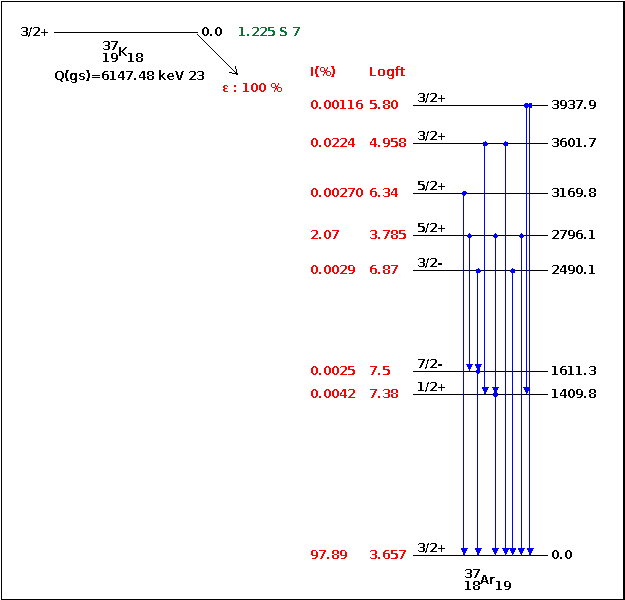
\includegraphics[width=.999\linewidth]{Figures/decayscheme_nndc.png}
%%	\note[orange, nolist]{Authors: John Cameron, Jun Chen and Balraj Singh, Ninel Nica.
%%	\\
%%	Citation:Nuclear Data Sheets 113, 365 (2012) \cite{nucleardata2012}.
%%	\\...\\
%%	Also, it's generated by the page from:  National Nuclear Data Center (NNDC) at Brookhaven National Laboratory.  Possibly from the NuDat3 database.
%%%	\\
%%%	https://www.nndc.bnl.gov/nudat3/decaysearchdirect.jsp?nuc=37K&unc=NDS
%%	}
%%	\caption[New 37K decay scheme]{A newer, better, less generated-by-Dan level diagram for the decay of $\isotope[37]{K}$.  \cite{nucleardata2012} \cite{ChinPhysC2012}. (probably only use the first citation?) }	
%%	\label{fig:nuclearleveldiagram_new}
%%\end{figure}


%%%%%%%%%%%%%%%%%%%%%%%%%%%
\FloatBarrier

\note[done, nolist]{Suggestions from John on listing my contributions that need to be mentioned and/or general stuff that needs to be mentioned:
\\
Georg wants you to list your contributions in the intro, good.
}

\note[moved, nolist]{First, in Section 2.4 the sentence after Harvey and Murray are referenced could be "There are some details of the present implementation of the AC MOT in Ref.~\cite{thesis}, done with a separate MOT geometry from
this beta decay work."
\\
(Presently your thesis is Ref. 14, which is only cited so far for Fig. 2.1)
\\...\\
*you need a subsection in Section 2.4 "The AC-MOT and Polarization" on your field trimming.
\\...\\
Time-constant ambient fields were trimmed in all dimensions using two horizontal pairs of Helmholtz coils and the AC MOT coils for the vertical direction.
These ambient B fields were first trimmed to be near zero using a giant magnetoresistance 3-axis probe at the trap center, with the MCP assembly removed and the vacuum chamber up to air.
\\...\\
Final trimming was done by optimizing polarization of stable $^{41}$K atoms with the apparatus assembled (cite[Fenker PRL Suppl Mat] has some details).
}
\note[moved, nolist]{The AC MOT and polarization B fields were generated by SRS DS345 arbitrary waveform generators, amplified by
Matsusada bipolar 20 KHz bandwidth 80A 20V amplifiers. The waveforms were carefully trimmed in amplitude and time to minimize B fields from eddy currents during the optical pumping cycle, again with the MCP assembly removed and the vacuum chamber up to air.
\\...\\
The bipolar amplifier bandwidth was inadequate when using current control mode, so voltage control had to be used, a much more time-exacting process requiring empirical iteration. These waveforms are not the same for the top and bottom coils, as during the optical pumping cycle one coil had to be flipped with respect to the MOT cycle to create the uniform vertical field for optical pumping by a Helmholtz rather than antiHelmholtz configuration.
\\
The beta detector full assemblies were in place during the field trimming.
\\...\\
All materials near the trap cloud are chosen to minimize both magnetic permeability to suppress time-constant B field gradients and conductivity to suppress eddy currents. E.g., the E field electrodes are made from either glassy carbon semiconductor or titanium alloy. A copper ring (not pictured in Fig. 2.5) with a slit mounted on each beta detector stainless steel reentrant flange suppresses the worst eddy currents fighting the B field along the z-axis. These designs were all confirmed by finite element calculations of another collaboration member.
}


\note[moved, nolist]{
I think you've neglected where the fT value and prediction for Abeta come from, entirely, and still don't have an equation for b\_Fierz in terms of Cs and Ct.
\\...\\
You had a note to do this, and in desperation I encouraged you to leave it out.
I was wrong and Georg is right-- the whole SM prediction for Abeta makes no sense this way, and something about it needs to be there.
\\...\\
there are two ways to add a dedicated section in ch 1:
\begin{itemize}
	\item i) by writing the equation for the rate in terms of Vud and rho (the G-T matrix element over Fermi squared), and saying Shidling et al. gets rho from that by assuming Vud from the 0+ to 0+ decays. (You had a note "Do the master equation!" which I think I said you needed to leave out, but I was probably wrong.) But then you have to define all the small corrections, which is a lot of physics.
	\item ii) Write the SM equation for Abeta in terms of rho, to give you the SM prediction for Abeta. State that recoil order corrections are in Appendix X. (If that's now a collaboration note? cite that there are recoil corrections considered in Appendix X-1 and a collaboration note).
	\item iii) Such a section would then naturally end with b\_Fierz in terms of Cs and Ct, a natural followup to what you've written.
	\\
"JTW does the Dirac matrix traces necessary to write down the decay rates in term of the Lee-Yang Lagrangian's parameters.
The prediction for b\_Fierz is " " which is zero in the SM." \textbf{even with recoil-order corrections} (there is no recoil order correction with the same m/Ebeta dependence).
\\
Then and only then will the final addition of the bFierz plot will make sense.
\end{itemize}
%
OR, more likely:
\\
\textbf{leave out i)}.
\\
Say in text that Shidling et al. (I've added the reference in a sticky note for the figure) hands you rho (the $M_{GT}/M_F$ ratio prediction) using as input the absolute rate, Vud from the 0+ to 0+ beta decays, and calculations of isospin mixing and radiative corrections (cite[shidling]) for details beyond the scope of this thesis. The sign of rho comes both from a shell model by Ian and by if it were flipped Abeta would be off by an enormous factor. 
\\...\\
Then you would just need \textbf{ii and iii}.
}
\note[jbn, nolist]{
As a reward for reading this far, I'll admit I wrote the bFierz m/E dependence wrong in the sticky notes in ch 1, sorry.
}

%%%
\note[moved, nolist]{first, actually, Ben writes a good summary of Ft mirror equation in terms of Ft0+ to 0+ in the PRL, you could just use that in Ch. 1 and it would help enormously. (Of course now I'm scared because it doesn't mention isospin mixing is different for 37K and the others, and that should be in the numerator as (Ft0to0/Ft37K) well as in rho, shouldn't it? I would need to compare to Shidling's expressions to sort this out.)
}
\note[moved, nolist]{
I said Ft wrong. I think you must know what to do.  
\\
F is the lepton phase space integral.
\\
(Decay rate)/F is then a dimensionless quantity proportional to |matrix element|$^2$, which you could call the intrinsic strength of the transition.
\\
People instead consider the inverse quantity denoted Ft defined as F*t\_1/2, so if log\_10(Ft) is smaller, the strength is larger.
\\...\\
So e.g. t\_1/2 is wildly different for the 0+ to 0+ decays (t1/2 for $^{14}$O is a minute, not a second like 38mK) but once you correct for the wildly different phase space (the Coulomb energies and therefore the decay Q-value smoothly grow, and phase space goes like $Q^5$) the Ft rates are close (closer once percent corrections from isospin mixing and nucleus-dependent radiative corrections are applied).
}
\note[moved, nolist]{
...
\\
(That equation is fine-- I was confused earlier.) You can mention that script{Ft} has isospin-breaking and other theory corrections beyond the scope of the thesis, and cite Shidling for those. This equation, along with the Abeta equation in terms of rho (you should not include the right-handed currents in Ben's Abeta equation and re-state that your thesis is working on scalar and tensor in your title) then sets up the inputs you need for the Abeta prediction.
}
%%%

\note[moved, nolist]{Chapter 2 corrections from John:
\\
all of these are trivial....
\\
\begin{itemize}
\item *section 2.1.3 "using a Helmoltz coil" add "but with currents in opposite direction." (saying it correctly here then implicitly defines anti-Helmholtz which you use correctly later for the AC MOT)
\item *It would be simplest to write down what you mean by a quadrupole field. You could say: "approximately in our geometry near the trap center
\\
$\vec{B} = 2 B_o z \hat{z} - (B_0 x \hat{x} + B_0 y \hat{y})$
\item *section 2.4 near end "divergencelessness" is not a word. It's obvious how to fix it ''since del dot B =0 in a current-free region..."
\item 2.5.1 "roughly" -> "approximately" The Efield is not rough at all, it's pretty good really. 
\\
Is the rMCP really just a 2-plate chevron in 2014? I don't remember. Why can't I find Ben's thesis?
\end{itemize}
}
\note[moved, nolist]{Chapter 2 corrections from John: (trivial...):
\\...\\
*2.5.1 state clearly in an extra paragraph at the end that the polarization-determining data was taken with the rMCP, while the Abeta and bFierz data were taken with the eMCP. The polarization was assumed to be the same during the Abeta+bFierz data. This is backed up by constant 41K polarization data for weeks
of optimization, with all optical pumping and B field switching parameters kept constant. Ambient magnetic field changes of 50 milliGauss could cause some polarization perturbations at the precision achieved, yet the stray fields are under control at that level. The TRINAT lab is in a basement well-shielded from the experimental hall by concrete with rebar, and though 50 mG fields are seen in that Hall from an open Helmholtz ion trap, they and the 5-ton crane produce negligible fields when measured at the atom trap. The cyclotron field makes 0.5 Gauss, predominantly vertical, and a smaller horizontal component, but trim Helmholtz coils at TRINAT are adjusted during calibrations with cyclotron on vs. off, and of course the cyclotron is on with constant field during the 37K delivery.
}
\note[moved, nolist]{a glaring omission:
\\
\textbf{You don't state the polarization achieved 99.1$\pm$0.1 percent anywhere that I can see., citing the publication.} You might also state that's important for Abeta but has much more precision than needed for the near-zero bFierz term.
\\...\\
You mention the polarization is different by approximately 0.3\% in Section 6.1 from the cut, but never say what P is.
\\...\\
Appendix A has ?? for a discussion of the changes of the polarization cut, so you need to clean up that \ref{}. It is presently in Section 6.1.
}

%%%%%%%%%%%%%%%%%%%
\note[moved, nolist]{Another Round of Thoughts from John!
\\...\\
Fitting Ben's data (using for the bFierz function my convolution of 1/E with a Clifford tail) as I've shown before, compare what happens if I let Abeta float, or if I then fix Abeta arbitrarily to that floated value.
\\
That's not a well-motivated thing to do on its own, but it's not that much different than using Abeta[Cs$^2$,Ct$^2$] constrained by Ft[Cs$^2$,Ct$^2$] since that's only dependent on squares of small quantities.
\\...\\
So I would expect the ability to extract Cs and Ct from the 37K data to have more
sensitivity if Abeta[Cs$^2$,Ct$^2$] and Ft[Cs$^2$,Ct$^2$] and bFierz[Cs,Ct] are floated together in a 2d fit rather then floating Abeta and bFierz without any theoretical constraints and then considering getting linear combinations of Cs and Ct from the bFierz value.
\\...\\
Note that my simply fixing Abeta lowers bFierz uncertainty by a factor of 3. I expect similar improvement in sensitivity to Cs and Ct.
\\...\\
(Here I'm using Cs as a stand-in for (Cs+Cs')/2 for simplicity)
}
\begin{figure}[htb]
	\centering
	\includegraphics[width=.999\linewidth]{Feedback/FixAndNot.png}
	\caption[A Fit From John - moved]{A Fit From John, or something -- moved.  idk, it goes with the text immediately previous.}
%	\label{}
\end{figure}
\FloatBarrier


\note[moved, nolist]{More thoughts from John:
\\...\\
hi Melissa,
\\...\\
I think you should keep Section 6.2, but I think it would be clearer to point out the observable manifests as a dip in the raw TOF spectrum, not going all the way to zero as in the ideal on-axis situation you describe for simplicity.
I.e., I would say you need to qualify this "exactly" word (emphasis mine below), and since
it ends up as a cos(theta) distribution like in my attached slide on the subject, your figure of the TOF spectrum would be a good way to do that.
\\...\\
"Henceforth, daughter nuclei from a back-to-back decay as shown in
Figure ?? will be described as ‘slow’ recoils. In terms of observables, this means that
if the electric field is configured to point along one of the axes perpendicular to the
polarization direction, then when the recoiling ion is swept away into a detector, the
slow recoil’s hit position should be \textbf{exactly}​​ along the projection of the polarization
axis. Furthermore, the slow recoil’s time of flight should be in the middle of the time
of flight spectrum, since other recoils will be emitted with momentum towards or
away from the detector"
}
\begin{figure}[htb]
	\centering
	\includegraphics[width=.999\linewidth]{Feedback/AMirrorDecayObservable.png}
	\caption[A Slide From John]{A Slide From John, or something -- moved  idk, it goes with the text immediately previous.}
%	\label{}
\end{figure}
\FloatBarrier





%%%% --- * --- %%%%	
%%%%%%%%%%%%%%%%%%%
%\FloatBarrier
\clearpage

\note[white, nolist]{Old Notes!} \noindent

\note[jb1, nolist]{JB on intuitive concepts that are missing (are they *still* missing?!?):  }
\note[done, nolist]{
The SM couples to left-handed neutrinos and right-handed antineutrinos. Since the neutrinos only have weak interactions, there are no right-handed nu's nor left-handed antinu's in nature. The neutrino asymmetry $B_\nu$ is a number with no energy dependence. 
\\...\\
Similarly, the SM weak interaction only couples to right-handed positrons and left-handed electrons. Since these are massive particles, the average helicity of positrons is not 1, but instead v/c. One can always boost to a frame where the positron keeps its circulation but is moving in the opposite direction. This is why the beta asymmetry is A v/c, not just A.
}
\note[jb1, nolist]{
The Fierz term's additional energy dependence of m/E also comes from helicity arguments, stemming from the fact that it still is coupling to SM nu's and antinu's only, so the beta's are generated with wrong handedness.  
\\...\\
The details are built at 4th-year undergrad level in Garcia's paper with his student and postdoc~\cite{hong_sternberg_garcia}.
}
%\note[jb1]{JB on intuitive concepts that are missing:  
%\\
%The beta asymmetry dependence on the Fierz term only comes through the normalization of $W(\theta) = 1 + \bFierz m/E + \Abeta \cos(\theta)$.
%\\ i.e.:
%\\$W'(\theta) = 1 + \Abeta/(1+ \bFierz m/E) \cos(\theta)$.  (the angular distribution must be unity where cos(theta) vanishes, by definition).
%}

.
\note[moved, nolist]{I have legit just deleted a section in Ch.6:  "Relation to Other Measurements and New Overall Limits".  It's gone now.  Because it was stupid.  Only John's comments about what it might do in the future remain.}
\note[moved, nolist]{JB on Ch.~\ref{sec:relation_to_other_measurements}:  "Relation to Other Measurements and New Overall Limits"
\\
6.3 might be better left to a collaboration memo. You have to decide what to do here,
and decide it quickly.
\\...\\
I already gave you the latest Perkeo Fierz paper,
and the info that we are relatively less sensitive to tensor by
by the ratio of Mgt$^2$ = 3/0.6 = 5.
\\...\\
so if you make a linearized exclusion plot of tensor vs. scalar as straight
lines with the uncertainty of bFierz, using Perkeo and your result, you
will see even with 0.09 uncertainty you compete with them on the scalar limit.
\\...\\
(However, see attached figure from my article with Alexandre on 38mK's
beta-nu scalar limit. I think the constraints on Lorentz scalars are hard to
compete with.)
}
\note[moved, nolist]{JB says:   To put your work in context, please add at the end of that minimal S,T section, or at the end of "Our Decay" section
\\ ... \\
The best existing measurement of $\bFierz$ is in the decay of the neutron~\cite{Saul2020},
$\bFierz$ = 0.017 $\pm$ 0.021, consistent with the Standard Model prediction of zero.
Our measurement is strongly related, yet complementary.
In terms on non-Standard Model Lorentz current structures, to lowest order in the non-SM  currents the same equation applies:
\\
$\bFierz$ = $\pm$ $(C_S +C_S' + (C_T - C_T') \lambda^2)/( 1 + \lambda^2)$
\\
(the plus is for $\beta^-$ decay and the - for $\beta^+$ decay)~\cite{jtw}.  [to be continued...] }
\note[moved, nolist]{[...continued from prev.]
\\
In our $^{37}$K case, $\lambda^2$ = $|M_{\rm GT}|^2$/$|M_{\rm F}|^2$ is close to 3/5 (the expected value j/(j+1) for a single j=3/2 d3/2 nucleon)~\cite{deShalit1963},
while for the neutron $\lambda^2$ is close to 3 (the expected value for an (j+1)/j j=1/2 s1/2 nucleon).
$|M_F|$, the Fermi matrix element, is nearly the same for both of these isospin = 1/2 decays (the largest correction is the larger isospin mixing of $\sim$0.01 in $^{37}$K).
So our observable is relatively less sensitive to Lorentz tensor currents, and will predominantly constrain or discover Lorentz scalar currents.
\\...\\ 
Full considerations would require a weighted fit of $\bFierz$ experiments and similar observables~\cite{Falkowski2021}, and are beyond the scope of this thesis.
The info from this thesis, values of $\Abeta$ and $\bFierz$ with their uncertainties, can together with the known $fT$ value (lifetime and
branching ratio) allow the community and/or the collaboration to include the results in a future constraint or discovery of scalar and tensor Lorentz currents
contributing to $\beta$ decay.}
\note[moved, nolist]{End of John's comments on the section I deleted.}






























%
%%%% --- * --- %%%%	
\clearpage
\section{Stuff that Remains after Round 0}

\subsection{Ch. 1}

%\note{...on the Four Forces}
% 4 forces

% Standard Model

%which includes quantitative models of 

% allows them to act even over long distances, as it implies that the amount of flux per unit solid angle is constant over all distance scales, leading to, e.g., the applicability of the famous Gauss's Law.  \aside{cite someone for Gauss's Law.}

%, which could be readily applied to the gravitational and electromagnetic forces, is no longer entirely straightforward to apply.  

%Despite the large number of possible weak force interaction vertices, 
%develop an intuition about the types of interactions that are possible (see Fig.~\ref{fig:feynmandiagrams_general}).  
%%%%\begin{figure}[h!tb]
%%%%	\centering
%%%%	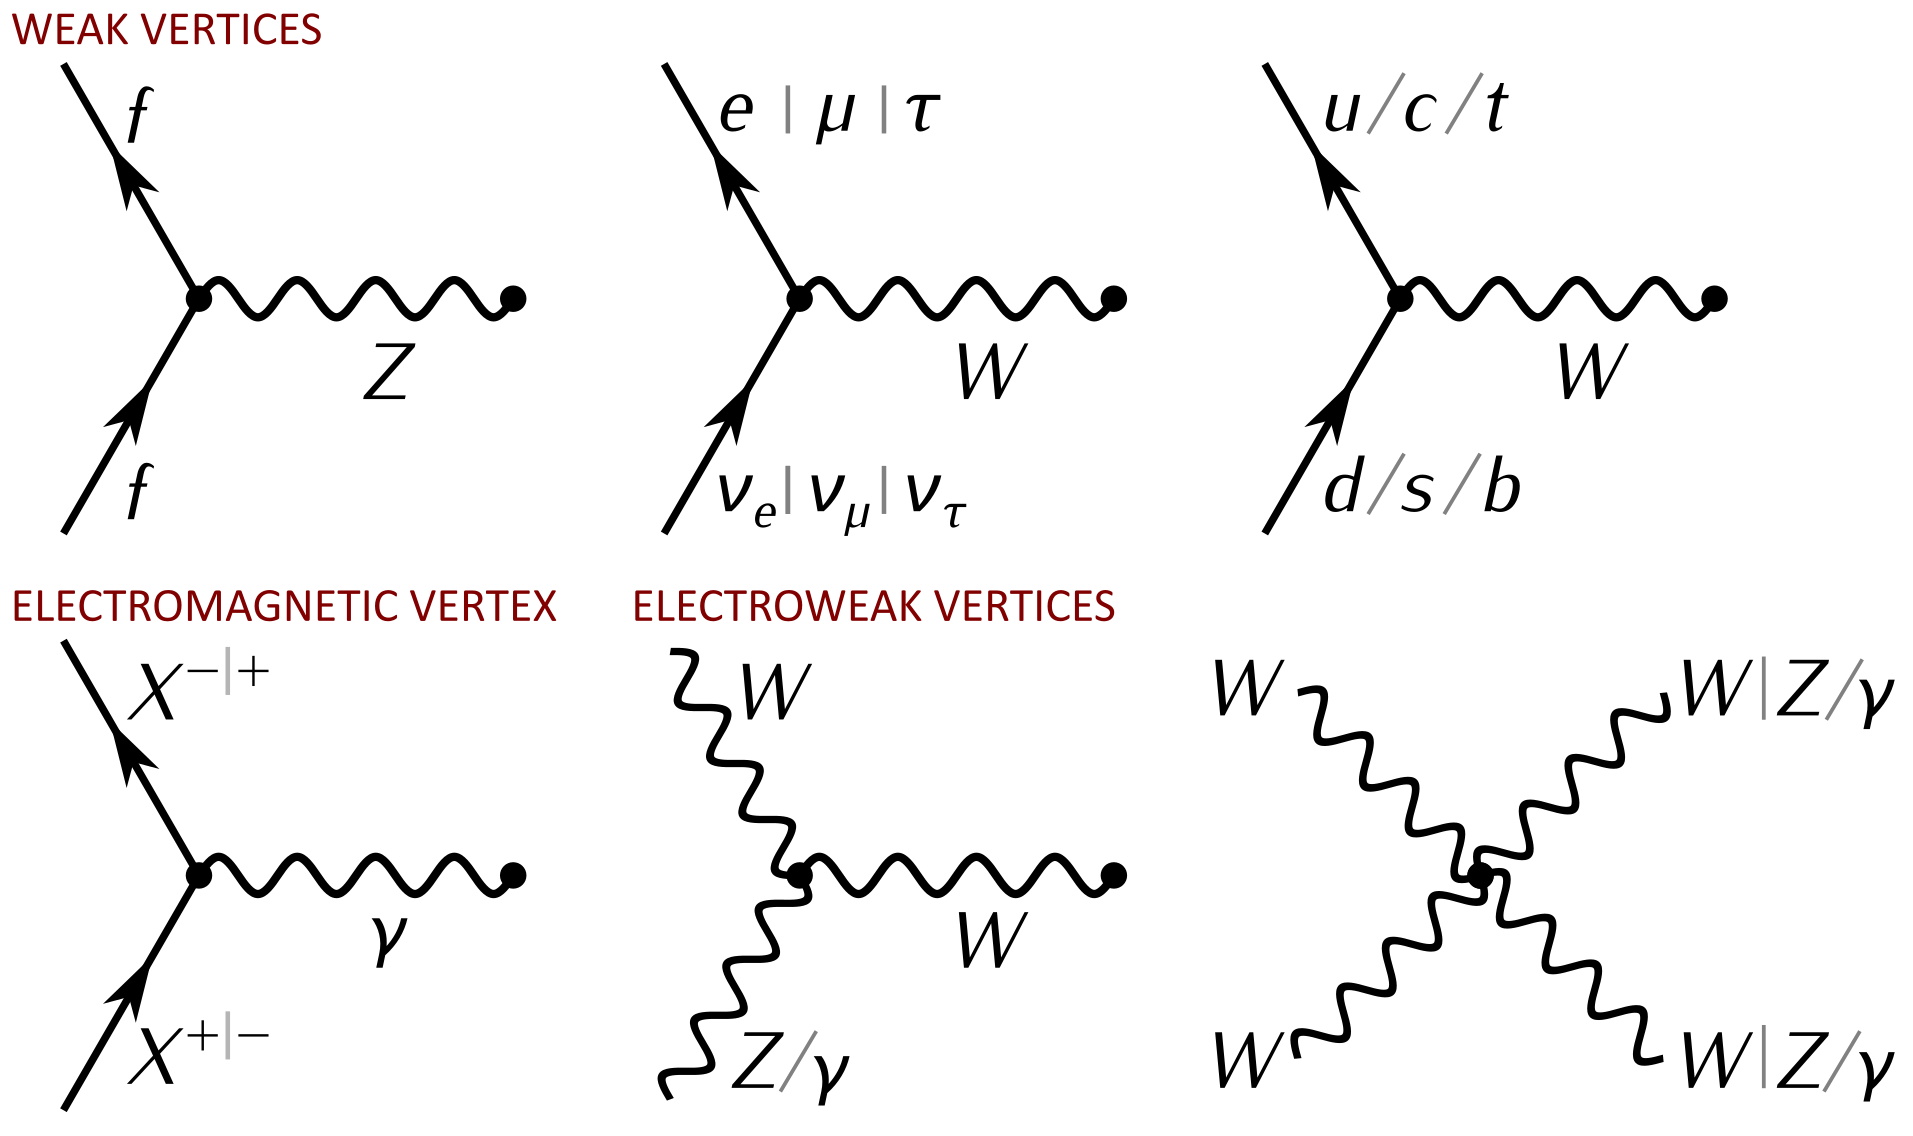
\includegraphics[width=.999\linewidth]{Figures/feynmanvertices_placeholder.png}
%%%%	\note{I have to re-make this figure.  This one doesn't belong to me.  Also, I'm not necessarily sure I believe/understand what it's saying on the bottom line.}
%%%%	\caption[Allowed Weak Vertices]{Allowed Weak Vertices:  a placeholder figure.  Top left:  $f$ is any fermion.  Top centre:  Lepton flavour is conserved under the weak interaction.  Top right:  quark generation is not conserved under the weak interaction.}	
%%%%	\label{fig:feynmandiagrams}
%%%%\end{figure}

%The beta decay process 
%certainly 

%It is these beta decay processes which present what is arguably the most accessible experimental window on the workings of the nuclear weak force.

%
%In Fig.~\ref{fig:feynmandiagrams_betadecay} the tree-level Feynman diagrams pertaining to the most common beta decay processes are shown.  
%%
%It is these beta decay processes which present what is arguably the most accessible experimental window on the workings of the nuclear weak force.
%
%
%\FloatBarrier
%\begin{figure}[h!t!b!]
%	\centering
%	\includegraphics[width=.90\linewidth]{Figures/feynmandiagrams_betadecay_placeholder.jpeg}
%	\note[tag]{Fix beta decay Feynman diagram placeholder figure.}
%	\caption[Beta Decay Feynman Diagrams]{Beta decay Feynman diagrams are shown here at the nucleon(? sort of) level.    
%	}	
%	\label{fig:feynmandiagrams_betadecay}
%\end{figure}
%
%
%The nuclear weak force is one of four fundamental forces described within physics.  
%It mediates the process of beta decay, which is of particular interest to us here.  

%form of the operators mediating the decay.  

%\aside{Something something ... it's so well understood that all that's left to do is the precision measurements.}

%\note[jbn]{Standard Model -> standard model of particle physics (often denoted here "SM"). 
%\\
%The standard model is ...
%\\...\\
%Weak -> weak.
%\\...\\
%This of course is the place where Georg wants more for orientation.
%}


%Attempting to unify the four fundamental forces within a single theoretical framework has been a major focus of later 20th- and early 21st century physics to date, however the effort has thus far been met with only partial success.


\note[orange, nolist]{
\begin{itemize}
	\item (we're not proposing a new feynman diagram.  Just, a new vertex factor thingy, I guess.)
	\item Weak force lagrangian!  I think possibly it's only for the *charged* weak force??
	\item ...then we demand that the Lagrangian must be Lorentz invariant, otherwise we break physics.
%	\item weak force moderated by massive particles -- so it can't be as long range, and Gauss's Law doesn't hold.
	\item within this thesis, we will focus primarily on the \emph{charged} weak interactions (using $W^{\pm}$ as mediators rather than $Z^0$), with first-generation normal matter quarks (\emph{i.e.} up ($u$) and down ($d$) quarks, but not charm ($c$), strange ($s$), top ($t$), or bottom ($b$) quarks; no anti-quarks ($\bar{q}$ for $q=\{u,d,c,s,t,b \}$ )) and first-generation leptons (\emph{i.e.} electrons, positrons, electron neutrinos and electron anti-neutrinos, but not positive or negative muons or taus, nor muon or tau neutrinos or anti-neutrinos).
	\item Really, we'll only be looking at weak force interactions involving the two most common nucleons -- protons and neutrons.  ...each of which is a (meta-)stable bound state involving three quarks.  
%	\item the weak force couples to both leptons and quarks.
	\item masses of W and Z bosons?  
%	\item graviton -- theoretical only.
%	\item strong force -- beyond the scope.
\end{itemize}
}


%%%%%Within the present understanding of physics, there are four fundamental forces governing the interactions of particles with one another:  electromagnetism, the nuclear weak force, the nuclear strong force, and gravity. 
%%%%%%
%%%%%Among other things, these four forces are considered distinct by virtue of the fact that each one couples to a different type of charge and is mediated by a different type of particle.  The result is that each force has potentially different behaviour at varying length scales.  
%%%%%%
%%%%%The most familiar example of this is a comparison between the forces of electromagnetism and gravity.  While the electromagnetic force couples to both positive and negative electric charges, and can therefore create both attractive and repulsive forces, the gravitational force couples only to (positive) mass, and the result is a force that is only attractive and never repulsive.  Both forces are mediated by massless particles (the photon and graviton, respectively), which implies that the strength of the two forces must fall off at the same rate as the distance between interacting bodies is increased.  In the case of the nuclear weak force, the mediator particles are massive, ...
%%%%%
%%%%%Attempting to unify the four forces within a single theoretical framework has been a major focus of later 20th- and early 21st century physics to date, however the effort has thus far been met with some limited success.


%Attempts to unify the four forces within a single model have been a major focus of 20th- and 21st century physics, }

%%%Both are mediated by massless particles (the photon and graviton, respectively)
%%%Because these are both mediated by massless particles (the photon and graviton, respectively), their behaviour 


%\section{An Abbreviated Look at the History of Beta Decay}
%\note[tag]{History section needs *all* the citations.}


% With our modern understanding of radioactive decay, we know that this of course could not have been beta decay, but rather a combination of alpha decay and spontaneous fission -- however it was this observation that set the field into motion.  

%\aside{That arxiv rando claims that the half-life thing was developed or hinted at by 1900 Rutherford, but who the fuck knows?}


%This was also the year when the electron capture mechanism for beta decay was first proposed by Gian-Carlo Wick.  

%standard model does not attempt address the force of gravity

%%
%%its introduction arguably marks the beginning of our modern understanding of the topic. 
%%With one of its major results, now commonly known as Fermi's Golden Rule, still routinely taught 

%With one of its major results --- now commonly known as Fermi's Golden Rule --- still applicable for many modern calculations~\aside{rephrase} due to its powerful predictive ability together with its generalized quantum mechanical approach to the problem, Fermi's model arguably marks the beginning of our modern understanding of beta decay (see Sec.~\ref{}).

%%%\note[done]{Pauli and the neutrino:  
%%%\\...\\
%%%Brown, L.M. (1978). "The idea of the neutrino". Physics Today. 31 (9): 23–28. Bibcode:1978PhT....31i..23B. doi:10.1063/1.2995181.~\cite{PauliNeutrino1978}}

%The introduction of Fermi's theory of beta decay arguably marks the beginning of our modern understanding of the field.  
%Now commonly known as Fermi's Golden Rule, 
%One of the major results in this is now commonly known as Fermi's Golden Rule,  

%Now known as Fermi's Golden Rule, the introduction of this model
%arguably marks the beginning of our modern understanding of beta decay.  Fermi's Golden Rule is both remarkably general in its approach and powerful in its predictive power, approaching the matter from a fully quantum mechanical perspective (see Section~\ref{}).~\aside{add link} 

%On the experimental front,~\aside{Rephrase.} 


%\note[done]{Asymptotic freedom as a thing was developed in 1973 by David Gross and Frank Wilczek\cite{gross1973asymptotically}\cite{gross1973ultraviolet}, and separately by David Politzer\cite{politzer1973reliable}. }
%\note[done]{They started calling it the standard model at some point during the 1970s.  One of the earliest records in print is from Treiman and Pais in 1975\cite{PaisTreiman1975}, but Weinberg claims to have used it during a talk in 1973~\cite{weinberginterview2018}.  On the other hand, Weinberg is old now and it's been many years, so there's that too.  }

%\note{What about the full SM, incorporating the strong force too?}
%\note[done]{....And then they included the model of the nuclear strong force too, turning it into one giant-ass model.  The Standard Model.  I could probably cite some people about how the term got coined, and what it refered to then and what it refers to now.}




%it was subsequently determined 
%\note{Feynman and Gell-Mann postulated the $V-A$ form of the interaction in 1958, by analogy with the E\&M photon\cite{FeynmanGellMann1958}.  }

%\note{}
%We must now backtrack slightly to account for modern theoretical development relating to beta decay.  
%describe the theoretical development that 
%Many of the subsequent developments in the field came 



%%%%%demonstrated unequivocally
%%%%%It was not 
%%%%
%%%%Steven Weinberg, too, stumbled upon the symmetries to needed to produce a unified electroweak force in 1967, and used it to (roughly) predict the masses of the $W^{\pm}$ and $Z^0$ bosons that had been postulated.  Weinberg further claimed -- but did not demonstrate -- that his theory was renormalizable, but it was not established mathematically until 1971, when Gerardus 't Hooft proved that theories within that class were renormalizable.~\aside{So this is electroweak theory.  Or sometimes, Weinberg-Salam theory.  Nobel prize went to Glashow, Salam, and Weinberg.}

%%%\note[done]{Higgs mechanism papers:
%%%\\...\\
%%%Englert, F.; Brout, R. (1964). "Broken Symmetry and the Mass of Gauge Vector Mesons". Physical Review Letters. 13 (9): 321–23. Bibcode:1964PhRvL..13..321E. doi:10.1103/PhysRevLett.13.321. \cite{Higgs1964EnglertBrout}
%%%\\
%%%Brout, R.; Englert, F. (1998). "Spontaneous Symmetry Breaking in Gauge Theories: A Historical Survey". arXiv:hep-th/9802142. \cite{BroutEnglertArXiv}
%%%\\
%%%Higgs, P. (1964). "Broken Symmetries and the Masses of Gauge Bosons". Physical Review Letters. 13 (16): 508–509. Bibcode:1964PhRvL..13..508H. doi:10.1103/PhysRevLett.13.508. \cite{Higgs1964Higgs}
%%%\\
%%%Guralnik, G.; Hagen, C. R.; Kibble, T. W. B. (1964). "Global Conservation Laws and Massless Particles". Physical Review Letters. 13 (20): 585–587. Bibcode:1964PhRvL..13..585G. doi:10.1103/PhysRevLett.13.585.  \cite{Higgs1964GuralnikHagenKibble}
%%%\\
%%%Guralnik, G. S. (2009). "The History of the Guralnik, Hagen and Kibble development of the Theory of Spontaneous Symmetry Breaking and Gauge Particles". International Journal of Modern Physics A. 24 (14): 2601–2627. arXiv:0907.3466. Bibcode:2009IJMPA..24.2601G. doi:10.1142/S0217751X09045431. S2CID 16298371. \cite{guralnik2009}
%%%}


%\note[done]{
%Salam and Weinberg apply the Higgs mechanism:
%\\...\\
% Weinberg, S. (1967). "A Model of Leptons". Physical Review Letters. 19 (21): 1264–1266. Bibcode:1967PhRvL..19.1264W. doi:10.1103/PhysRevLett.19.1264. \cite{Weinberg1967}
%\\ ... \\
%Salam, A. (1968). Svartholm, N. (ed.). Elementary Particle Physics: Relativistic Groups and Analyticity. Eighth Nobel Symposium. Stockholm: Almquvist and Wiksell. p. 367.  \cite{salam1968}
%}

%%%\note[done]{ 't Hooft + Veltman renormalize shit:
%%%\\...\\
%%%t Hooft, G.; Veltman, M. (1972). "Regularization and renormalization of gauge fields". Nuclear Physics B. 44 (1): 189–213. Bibcode:1972NuPhB..44..189T. doi:10.1016/0550-3213(72)90279-9. hdl:1874/4845. \cite{thooftveltman1972}
%%%}

%Sheldon Glashow in 1961 extended some of Schwinger's work to model the nuclear weak force, 
%with a manually broken symmetry that able to represent the $W^+$ and $W^-$ bosons involved in beta decay, and for the first time, the neutral $Z^0$ boson.
%predicting the $W^+$ and $W^-$ bosons involved in beta decay, and for the first time, the neutral $Z^0$ boson.  
%The theory was not renormalizable, and 
%since there had not been any experimental hint of the $Z^0$, even Glashow himself discounted the model, and it initially received little attention.  
%In 1964, Abdus Salam and John Clive Ward made a similar prediction, this time including the photon --- but as they still relied on manual symmetry breaking, this theory also was non-renormalizable.  

%It was Steven Weinberg who, while investigating ...



%%%\note[done]{References for first sentence:
%%%\\ ... \\
%%%S. Tomonaga (1946). "On a Relativistically Invariant Formulation of the Quantum Theory of Wave Fields". Progress of Theoretical Physics. 1 (2): 27–42. doi:10.1143/PTP.1.27. \cite{tomonaga1946}
%%%\\
%%%J. Schwinger (1948). "On Quantum-Electrodynamics and the Magnetic Moment of the Electron". Physical Review. 73 (4): 416–17. doi:10.1103/PhysRev.73.416. \cite{schwinger1948magnetic}  (Really?  Do I really want to cite this thing, given the other thing? ... no, I don't think so.)
%%%\\
%%%J. Schwinger (1948). "Quantum Electrodynamics. I. A Covariant Formulation". Physical Review. 74 (10): 1439–61. doi:10.1103/PhysRev.74.1439.,  \cite{schwinger1948covariant}
%%%\\
%%%R. P. Feynman (1949). "Space–Time Approach to Quantum Electrodynamics". Physical Review. 76 (6): 769–89. doi:10.1103/PhysRev.76.769., \cite{feynman1949spacetime}  (Yeah, I think this is relevant.)
%%%\\
%%%R. P. Feynman (1949). "The Theory of Positrons". Physical Review. 76 (6): 749–59. doi:10.1103/PhysRev.76.749., \cite{feynman1949positrons}  (Possibly less relevant?)
%%%\\
%%%R. P. Feynman (1950). "Mathematical Formulation of the Quantum Theory of Electromagnetic Interaction" (PDF). Physical Review. 80 (3): 440–57.  doi:10.1103/PhysRev.80.440.,  \cite{feynman1950}
%%%\\
%%%F. Dyson (1949). "The Radiation Theories of Tomonaga, Schwinger, and Feynman". Physical Review. 75 (3): 486–502. doi:10.1103/PhysRev.75.486., \cite{dyson1949theories}
%%%\\ ... \\
%%%Also, do I maybe want to look at Dyson's thing that might actually be more relevant?  \cite{dyson1949Smatrix}.  Nope.  I don't think so.  Maybe I don't want to mention him by name at all.
%%%}

%\cite{Weinberg1967}. \aside{Something is wrong here -- this is the wrong Weinberg citation...}

%%\note[done]{References:  second paragraph:
%%\\ ... \\
%%Glashow, Sheldon L. (February 1961). "Partial-symmetries of weak interactions". Nuclear Physics. 22 (4): 579–588. doi:10.1016/0029-5582(61)90469-2. Archived from the original on 2021-02-27. Retrieved 2020-12-02.  \cite{Glashow1961} 
%%\\
%%Salam, A.; Ward, J.C. (November 1964). "Electromagnetic and weak interactions". Physics Letters. 13 (2): 168–171. doi:10.1016/0031-9163(64)90711-5.  \cite{SalamWard1964}  (this one is already in?)
%%\\
%%Weinberg, S (1967). "A Model of Leptons" (PDF). Phys. Rev. Lett. 19 (21): 1264–66. doi:10.1103/PhysRevLett.19.1264. \cite{Weinberg1967}  (this one is already in?)
%%}







%\note{W and Z bosons not experimentally observed until 1983.  (Or possibly 1986?)
%\\
%Cottingham, W.N.; Greenwood, D.A. (2001) [1986]. An introduction to nuclear physics (2nd ed.). Cambridge University Press. p. 30. ISBN 978-0-521-65733-4. }
%
%
%\note{The neutral current was measured first at CERN in 1973, with Gargamelle\cite{gargamelle}.  W bosons, and soon afterwards, Z bosons were experimentally measured for the first time in 1983, using the Super Proton Synchrotron.  }

%\note{}

%\note[done]{OK, how/when did they do electroweak unification, and who did it?---Glashow+Weinberg+Salam, 1968.}


%%%He named this particle a "neutron", though he was referring to the particle we refer to today as the "neutrino".  
%%%
%%%(which he referred to as a "neutron" at the time, though we now call it a neutrino, and use the term "neutron" to describe something else)
%%%
%%%
%%%a neutrino (which he referred to as a "neutron" at the time) 

%\subsection{bullet points.}
%%Beta Decay:
%%\begin{itemize}
%%\item 1931 - Pauli "discovers" neutrinos and is very confused.
%%\item 1934 - Fermi's Golden Rule to describe the rate of beta decay in terms of transition matrix elements.
%%\item ...
%%\item 1956 - Lee and Yang wonder if parity is even conserved in beta decay?  
%%\item 1957 - C.S. Wu shows that parity isn't conserved.  At all.
%%\item ???? - turns out it's V-A.
%%\end{itemize}
%Standard Model:
%\begin{itemize}
%\item ???? - Schwinger 
%\item 1959 - Glashow
%\item 1964 - Salam and Ward
%\item 1967 - Weinberg
%\item 1971 - 't Hooft
%\item ...
%\item 1954 - Yang + Mills  .... huh?
%\end{itemize}
%%Radioactivity:
%%\begin{itemize}
%%\item 1896 - Henry Bequerel in Uranium.  Presumably that's alpha decay.
%%\item 1898 - Thorium is radioactive -- Marie Curie + Gerhard Carl Schmidt, independently.
%%\item 	 - Curie:  Thorium, polonium, radium -- all radioactive!
%%\item 1899 - Rutherford notices that there's two types of emissions:  alpha and beta (beta minus).
%%\item 1900 - Paul Villard discovers gamma rays, doesn't realize they're different?  Or something?
%%\item 1903 - Rutherford realizes that gamma rays are a fundamentally new thing.
%%\item ...
%%\item 1900 - Becquerel realizes beta particles have the same charge-to-mass ratio as electrons, postulates that they're the same thing.
%%\item 1901 - Rutherford + Soddy show that alpha and beta decay turn elements into different elements.  
%%\item ...
%%\item 1911 - Lise Meitner + Otto Hahn:  emitted beta particles come out at many different energies.  Unlike alpha and gamma decays.
%%\item 1914 - James Chadwick shows that it's a continuous distribution.
%%...
%%\item 1930 - Pauli proposes neutrinos (but he called them "neutrons") as a solution to the missing energy problem.
%%\item 1931 - Fermi calls them neutrinos.  
%%\item 1933 - Fermi's landmark theory?  Surely it's 1934.
%%...
%%\item 1934 - Irène and Frédéric Joliot-Curie discover (induced) beta+ decay.  it got 'em a nobel prize.
%%\item 1934 - Wick proposes electron capture as a thing.  Yukawa and others maybe have thoughts about that too.
%%\item 1937 - Luis Alvarez observes electron capture.
%%\item ???? - Parity?  Coupling constants??
%%\end{itemize}


\FloatBarrier
%%%% --- * --- %%%%	
%%\ifthenelse{\boolean{isdraft}}
%%{
\subsubsection{Beta Decay within the Standard Model -- a section that no longer exists.}
\note[tag]{This section is problematic....}
%\note{Intro blurb goes here.
%\\...\\
%The most general and vague description of beta decay ever:  a proton turns into a neutron and emits a positron, or else a neutron turns into a proton and emits an electron.  Also, neutrinos are emitted with the proton/electron.  Occasionally, also, an electron from like atomic orbitals or something gets captured, triggering a similar process in which a proton is transmuted into a neutron, but no positron/electron gets emitted.  A neutrino does though.  The Feynman diagrams for all these things are pretty similar, and they're shown in Fig.~\ref{fig:feynmandiagrams_betadecay}.  
%\\..\\
%Electric charge is kept fixed.  The whole process is mediated by the $W^\pm$ bosons.  
%}
%%%%%%%%%
%\note{}
%\note{Imported figure and reference to the figure are here.  It probably goes in this section rather than the one it was in before.}
%In Fig.~\ref{fig:feynmandiagrams_betadecay} the tree-level Feynman diagrams pertaining to the most common beta decay processes are shown.  
%%
%It is these beta decay processes which present what is arguably the most accessible experimental window on the workings of the nuclear weak force.
%
%\FloatBarrier
%\begin{figure}[h!t!b!]
%	\centering
%	\includegraphics[width=.90\linewidth]{Figures/feynmandiagrams_betadecay_placeholder.jpeg}
%	\note[tag]{Fix beta decay Feynman diagram placeholder figure.}
%	\caption[Beta Decay Feynman Diagrams]{Beta decay Feynman diagrams are shown here at the nucleon(? sort of) level.    
%	}	
%	\label{fig:feynmandiagrams_betadecay}
%\end{figure}
%\note{}
%%%%%%%%%
%
%A nucleus undergoing beta decay converts one of its protons (neutrons) into a neutron (proton), and simultaneously emits a lepton and anti-lepton.  The daughter nucleon remains bound in place of its parent, and the overall electric charge of the nucleus is changed by -1 (+1), with the extra charge being carried away by the anti-lepton (lepton).  In particular, at the nucleon level, three beta decay processes are possible:
%\bea
%	p &\rightarrow& n + e^+ + \nu_e        \label{eq:betaplus_decay} \\
%	n &\rightarrow& p + e^- + \bar{\nu}_e, \label{eq:betaminus_decay}  \\
%	p + e^- &\rightarrow& n + \nu_e        \label{eq:electroncapture}
%\eea
%where the processes described in Eqs.~\ref{eq:betaplus_decay} and~\ref{eq:electroncapture} are energetically disallowed for an unbound proton, however there is no similar requirement for Eq.~\ref{eq:betaminus_decay}.
~\aside[jbn]{Eqs. ~\ref{eq:betaplus_decay} and ~\ref{eq:electroncapture} are energetically disallowed for an unbound proton, but allowed energetically when bound in nuclei as in 37K decay.}
\note[jbn]{Electron capture decay of Eq. 1.3 is calculated to be an 0.080\% branch compared to positron decay in 37K decay (Table VII of N. Severijns, M. Tandecki, T. Phalet, and I.S. Towner)~\cite{SeverijnsTandecki2008}, an important correction when interpreting the total decay rate of 37K to determine the theoretical prediction for 37K Abeta  (P.D. Shidling, R.S. Behling, B. Fenker, J.C. Hardy, V.E. Iacob, M. Mehlman, H.I. Park, B.T. Roeder, D. Melconian Phys Rev C 98 015502 (2018)~\cite{shidling2018}; A. Ozmetin, D.G. Melconian, V.E. Iacob, P. Shidling, V.S. Kolhinen, D.J. McClain, M. Nasser, B. Schroeder, B. Roeder, H. Park, M. Anholm, A.J. Saastamoinen, APS DNP Abstract KF.00005 2020 ``Improving the ft value of 37K via a precision measurement of the branching ratio'')~\cite{ozmetin2020}.
}
Limiting the focus of this discussion to Eq.~\ref{eq:betaplus_decay}, we note that this expression provides no information at all about the momenta or spin of the outgoing daughter particles.  This behaviour is governed by the form of the Weak coupling that mediates the decay.  

Within the field of nuclear physics, it is common to classify beta decay processes as being either ``Allowed'' or ``Forbidden''~\aside[jbn]{don't capatalize "Allowed" and "Forbidden."
The quotes are justified.} (sometimes with an associated number to describe the extent to which it is Forbidden), where Forbidden processes are generally suppressed but not truly forbidden.  In an Allowed transition, the positron and anti-neutrino are treated as being created at the nuclear centre, and as a result they may not carry away any \emph{orbital} angular momentum.  However, since the outgoing leptons both have spin $S=1/2$, it is still possible for the total nuclear angular momentum, $J$, to be changed in an Allowed decay.  This implies that an Allowed transition must \emph{always} change the total nuclear angular momentum by either $0$ or $\pm1$.  
~\note[jbn]{First forbidden decay emits leptons with total orbital angular momentum 1, changing the nuclear parity-- suppressed in a long-wavelength approximation ~ ((beta momentum)/(hbar c))$^2$ or about two orders of magnitude. This is one reason decays to negative-parity excited states of 37K are so small (Fig.~\ref{fig:nuclearleveldiagram}).
}

The Allowed decays traditionally are further separated into a Fermi singlet~\aside[jbn]{singlet in lepton spin} in which there is no change to nuclear angular momentum ($\Delta J = 0$) and therefore the two leptons are required to have anti-parallel spins, and a Gamow-Teller triplet~\cite{severijns_beck_cuncic_2006}, where the projection of the nuclear angular momentum is changed by $\pm1$.%, and so the two lepton spins must be aligned in parallel to one another under the Allowed approximation.
\note[done]{My only comment is to ask where the Fermi "singlet" and "triplet" came from, referring to coupling of the lepton spins.
\\
I have not seen this-- it could be fine, yes, I don't know.}

This implies that the total nuclear angular momentum is changed by $\Delta J = \{0, \pm1\}$ during a Gamow-Teller transition.  A mixed transition is also possible, however we note that the $J_i = J_f = 0$ decays must always be pure Fermi transitions, because there is no way to produce this result from two outgoing leptons with parallel spins.~\cite{krane}~\cite{wong1990}~\cite{severijns_beck_cuncic_2006}.

Given the differing behaviour within the angular momenta of the daughters in Fermi and Gamow-Teller transitions, it is perhaps not suprising that that the \emph{linear} momenta of the outgoing particles should also follow a different set of distributions in these two cases.  At the level of the Weak~\aside[jbn]{Don't capitalize Weak anywhere, either. You can keep quotes around the first "weak", I guess.} coupling, Fermi- and Gamow-Teller~\aside[jbn]{you should indeed capitalize Fermi and Gamow-Teller because these are people.} transitions are governed by different operators, with the Fermi interaction mediated by a so-called ``vector'' ($V$) coupling, and the Gamow-Teller interaction mediated by an ``axial-vector'' ($A$) coupling.
~\note[jbn]{The vector and axial-vector couplings refer to Lorentz transformation of the Lagrangian terms involved, which we come to next.}

%%}
%%{}  % End "if draft" section...



%%%% --- * --- %%%%	
%%%\section{On Modern Precision Measurements and the Nuclear Weak Force}
%%%\label{sec:modernprecision}
%%%Although the physics community has largely come to a consensus over the years about the \emph{dominant} behaviour of the nuclear weak force, there still exists a range of possible \emph{sub-dominant} behaviours that cannot be ruled out by theoretical considerations alone, and therefore must be tested experimentally.  With the weak force already so well described, searching for indications of unexpected behaviours is the domain of precision measurements.  This class of non-dominant behaviours is sometimes described as exotic physics, or with the imprecise label of physics \ac{BSM}, or even the wildly inaccurate misnomer, ``new physics''.  
%%%
%%%Many types of exotic physics have, in fact, already been described by Lee and Yang's 1956 interaction Hamiltonian, which was originally motivated by the question of parity conservation within beta decay\cite{LeeYang}.  Despite the original motivations, the authors were very thorough in their description of possible interaction types.  By starting with Fermi's contact interaction model of beta decay, incorporating Gamow and Teller's selection rules, and enforcing Lorentz invariance, they arrived at a nucleon-level Hamiltonian (quarks had not been discovered yet) which accounted for \emph{all} possible coupling behaviours~\cite{GamowTeller}. 
%%%%\aside{also cite Fermi here, and Gamow-Teller.}
%%%
%%%In the years since, we have discovered that beta decay is mediated by $W^\pm$ bosons, which, among other things, allows for the possibility of certain transitions (ie, with different selection rules) occuring, which had been considered forbidden under the contact interaction model.  
%%%%certain suppressed transitions with different selection rules
%%%%creates the opportunity for certain suppressed transitions to occur which follow different sets of selection rules.
%%%%thereby allowing for certain suppressed transitions with different sorts selection rules.  
%%%Since $W^\pm$ bosons are quite massive,
%%%%relative to typical beta decay energies,
%%%\aside{Give numbers.} the beta decay interaction is only applicable at a short range, and as a result, the Fermi model (with the Gamow-Teller addendum) represents a very good approximation for the transitions it applies to. \aside{Give numbers.}
%%%%So although Fermi's model with the Gamow-Teller addendum is not truly a complete description, it is still a very good approximation, given the mass of the  $W^\pm$ bosons relative to typical beta decay energies.
%%%\aside{Also, like many mathematical descriptions where one wants to predict things, it's better without the quarks.}
%%%%\note{This isn't quite right.  Gamow and Teller added a process to change nucleon spin, and the Lee-Yang Hamiltonian is based on that.}
%%%
%%%We begin with Fermi's\aside{Is this true?  Probably} description of the transition: 
%%%\bea
%%%\mathcal{M}_{fi} &=& G_F \int \bar{\psi}_f \, \mathcal{\hat{O}} \, \psi_i \,\textrm{d}V,% \;\;=\;\; \int \mathcal{H}_{\mathrm{int}} \textrm{d}V
%%%\eea 
%%%where $\mathcal{M}_{fi}$ is the transition matrix element between the final ($\psi_f$) and initial ($\psi_i$) states, and $G_F$ gives a measure of the size of the coupling between states.  The integral is evaluated over phase space volume.  Equivalently, $\mathcal{M}_{fi}$ may be written in terms of the interaction Hamiltonian $\mathcal{H}_{\mathrm{int}}$, as 
%%%\bea
%%%\mathcal{M}_{fi} &=& \int \! \mathcal{H}_{\mathrm{int}} \, \textrm{d}V. 
%%%%\label{eq:transitionmatrixhamiltonian}
%%%\eea 
%%%%
%%%This leads immediately to Fermi's Golden Rule, 
%%%\beq
%%%\Gamma \;\; = \;\; \frac{1}{\tau}  \;\; = \;\; \frac{2\pi}{\hbar} \left| \mathcal{M}_{fi} \right|^2 \, \rho(E_f),
%%%%\;\;\;\; \textrm{(Why is this formatted weird??)},
%%%\eeq
%%%which describes the relationship between the total transition rate $\Gamma$ (or equivalently the lifetime $\tau$), the transition matrix element $\mathcal{M}_{fi}$, and the available density of states at the final energy, $\rho(E_f)$.  We can also use this to write down the differential decay rate, 
%%%\bea
%%%\frac{\textrm{d}^5 \Gamma}{ \textrm{d} \Ebeta \textrm{d}\Omegahatbeta \textrm{d} \Omegahatnu } 
%%%&=& \frac{1}{(2\pi)^5} \, \pbeta \Ebeta (E_0 - \Ebeta)^2 F_{\pm}(\Ebeta, Z^\prime) \left| \mathcal{M}_{fi} \right|^2,
%%%%\frac{\textrm{d}^5 \Gamma}{ \textrm{d} \Ebeta \textrm{d}\Omegahatbeta \textrm{d} \Omegahatnu } 
%%%%&=& \frac{G_F^2}{(2\pi)^5} \, \pbeta \Ebeta (E_0 - \Ebeta)^2 F_{\pm}(\Ebeta, Z^\prime) \left| \mathcal{M}_{fi} \right|^2,
%%%\eea
%%%where \aside{pretty sure I lost an $\hbar$.  Maybe no one will notice.  }
%%%%$G_F$ is the mumble mumble,\aside[tag]{Fix $G_F$ !} 
%%%$\Ebeta$ and $\pbeta$ are the outgoing $\beta$'s (total) energy and momentum,
%%%$E_0$ is the maximum possible $\beta$ energy associated with the transition, 
%%%and $\FFpm$ is called a Fermi function (with $Z^\prime$ the proton number of the daughter), %\aside[tag]{$Z^\prime$ ?} 
%%%and is used to account for the electric force between the nucleus and the (charged) outgoing electron (top) or positron (bottom) \cite{Fermi1934Italian}\cite{Fermi1934German}\cite{krane}.  
%%%
%%%With this description, the problem of characterizing the transition is reduced to determining the form of $\mathcal{\hat{O}}$, or equivalently, $\mathcal{H}_{\mathrm{int}}$.  Table~\ref{table:dirac_matrix_operators} provides a comprehensive list of all operators for which Lorentz invariance holds.  The complete transition operator $\mathcal{\hat{O}}$ must be comprised of a linear combination of these terms.  
%%%% !TEX root = ../thesis_main.tex
%
%
%
%%%% --- * --- %%%%	
%\renewcommand{\arraystretch}{1.6}
\begin{table}[h!!!!t]
	\begin{center}
	\begin{tabular}{ l  l  l}
		\multicolumn{3}{l}{ \textbf{Lorentz Invariant Operators}}
		\\  %\hline
		\multicolumn{1}{l}{Name} 		& \multicolumn{1}{l}{ Form}   								& \multicolumn{1}{l}{Parity}   	
		\\  \hline
		%%% % %%%
		Scalar 			   				& $1$														& $+$									
		\\
		Pseudoscalar \;\;\;\;\;\;\;		& $\gamma_5$									 			& $-$				
		\\
		Vector							& $\gamma_\mu$												& $-$				
		\\
		Axial-vector					& $\gamma_\mu \gamma_5$										& $+$
		\\
		Tensor							& $\gamma_\mu \gamma_\nu - \gamma_\nu \gamma_\mu$ \;\;		& N/A									
		\\  \hline
		%%% % %%%
	\end{tabular}
	\end{center}
%	\caption[Dirac Matrix Operators]{Dirac Matrix Operators.  I need to reference this table somewhere.  Also, these are dirac matrices in 4D.  More D, different Dirac matrices.}
	\note{Ugh, I've largely just avoided talking about parity....}
	\caption[Lorentz Invariant Operators]{A complete list of operators that obey Lorentz invariance, defined in terms of Dirac $\gamma$-matrices~\cite{ben_thesis,dan_thesis}.  It can be shown that the operators listed here span the entire space, meaning that any other Lorentz invariant operator can be expressed as a sum of the above. }
%%%%%	as a result of certain symmetries in the Dirac matrices that all other Lorentz invariant operators can be reduced to these.}
	\label{table:dirac_matrix_operators}
\end{table}
%\renewcommand{\arraystretch}{1} % table:dirac_matrix_operators
%%%This gives rise to the Lee-Yang interaction Hamiltonian, which provides a generalized combination of the Lorentz invariant operators and fits neatly into Eq.~\ref{eq:transitionmatrixhamiltonian}~\cite{LeeYang}:
%%%
%%%%The Lee-Yang interaction Hamiltonian is: %\aside{It's an *interaction* Hamiltonian!}
%%%% !TEX root = ../thesis_main.tex
%
%
%%%% --- * --- %%%%	
\bea
{\mathcal H} &=& (\bar{\psi}_p \psi_n)( C_S \,\bar{\psi}_e \psi_\nu + C_S^\prime \, \bar{\psi}_e \gamma_5 \psi_\nu )
%
\nonumber \\ &&
+ \: (\bar{\psi}_p \gamma_\mu \psi_n)( C_V \,\bar{\psi}_e \gamma_\mu \psi_\nu + C_V^\prime \, \bar{\psi}_e \gamma_\mu \gamma_5 \psi_\nu )
%
\nonumber \\ &&
+ \: \frac{1}{2} (\bar{\psi}_p \sigma_{\lambda \mu} \psi_n)( C_T \,\bar{\psi}_e \sigma_{\lambda \mu} \psi_\nu + C_T^\prime \, \bar{\psi}_e \sigma_{\lambda \mu} \gamma_5 \psi_\nu ) 
%
\nonumber \\ &&
+ \: (\bar{\psi}_p \gamma_\mu \gamma_5 \psi_n)( C_A \,\bar{\psi}_e \gamma_\mu \gamma_5 \psi_\nu + C_A^\prime \, \bar{\psi}_e \gamma_\mu \psi_\nu )
%
\nonumber \\ &&
+ \: (\bar{\psi}_p \gamma_5 \psi_n)( C_P \,\bar{\psi}_e \gamma_5 \psi_\nu + C_P^\prime \, \bar{\psi}_e \psi_\nu ) 
%
+ \textrm{H.C.},
\label{eq:lee_yang_hamiltonian} 
\eea
%%%%  \label{eq:lee_yang_hamiltonian} 
%%%
%%%Here, $C_X$ and $C_X^{\prime}$ (with $X=\{V,A,S,T,P\}$) are complex coupling constants for vector, axial, scalar, tensor, and pseudoscalar interactions, and $\psi_Y$ (with $Y=\{p,n,e,\nu\}$) are the wavefunctions for the interaction's proton, neutron, electron, and neutrino.  Operators $\gamma_5$ and $\gamma_\mu$ are Dirac gamma matrices, and $\mbox{$\sigma_{\lambda\mu} = -\frac{i}{2}(\gamma_\lambda \gamma_\mu - \gamma_\mu\gamma_\lambda )$}$.  As usual, ``H.C.'' represents the Hermitian conjugate of the previous terms within the Hamiltonian.
%%%%\aside{What about sigma!?  is it a pauli matrix?}  
%%%
%%%The fact that there are two coupling constants (primed and unprimed) for each type of coupling relates to the \emph{handedness} of the interaction.  Both left-handed and right-handed couplings, or a combination thereof, are \emph{a priori} possible, and the form of Eq.~\ref{eq:lee_yang_hamiltonian} does not give preference to either.
%%%
%%%
%%%While it is possible to define an interaction's handedness in a rigorous and mathematical way, the reader may gain more clarity by simply remembering the rule of thumb that a left-handed weak force 
%%%% (which is predominantly or entirely what exists in nature) 
%%%couples only to left-handed regular matter leptons and right-handed anti-leptons --- where the handedness of a lepton or other particle is defined by the direction of its spin relative to its direction of motion.  That description is exact in the limit where such a lepton travels at the speed of light (otherwise a clever Lorentz transform can change the result), but the underlying mathematics is well defined for slower particles as well.  For neutrinos, which are so light they were long believed to be massless, the description is \emph{nearly perfect}.  For electrons and positrons emitted in beta decay, which are massive but often emitted at relativistic speeds, the description is only \emph{pretty good}.  
%%%
%%%
%%%\note{Here, we should put in Falkowski's convention to separate out the RH and LH components of things.  Or take it out completely.}
%%%
%%%%were long believed to be massless 
%%%% --- meaning that it is \emph{very good} for neutrinos emerging from a weak interaction, and \emph{pretty good} for electrons and positrons emerging from a similar interaction.  
%%%%
%%%%regular matter neutrinos that have a left-handed spin relative to the direction of motion
%%%%This can be defined in a rigorous and mathematical way, 
%%%%\note{The primes or lack thereof are a thingy with the interaction's handedness...}
%%%%$\psi_Y$ (with $Y=\{p=$proton, $n=$neutron, $e=$electron, $\nu=$neutrino$\}$)
%%%%the search for small deviations from this model is ongoing.  
%%%
%%%Over the years, the physics community has learned much about which simplifications to Eq.~\ref{eq:lee_yang_hamiltonian} can be justified.  Typically, reference to the pseudoscalar couplings is one of the first things to be dropped, because it is suppressed at typical beta decay energies, and as such its presence would be difficult to demonstrate and have very little effect on experimental results.  
%%%%Experimental results have demonstrated that 
%%%It is also now widely understood that 
%%%the nuclear weak force involves primarily (or entirely) vector and axial vector couplings, and is primarily (or entirely) a left-handed interaction in which parity is maximally (or nearly maximally) violated.  
%%%
%%%\note{We'll use Falkowski's convention to re-wite the Lee-Yang Hamiltonian in terms of right- and left-handed interactions.  That'll be useful later.  Sort-of.}
%%%
%%%\note{Something about how beta decays turned out to be $(V-A)$...}
%%%
%%%%\note{btw:  as of 2018, we have $m_W = 80.379(12)$\,GeV/$c^2$ ~\cite{pdg2018}.}

%%%% --- * --- %%%%	
%%%OK.  This stuff is basically yoinked from Ben's thesis.  And Dan's.  I'll need to re-organize and rephrase the content -- but I want to make sure I get the important points down.  
%%%
%%%In 1931, Pauli figured out about neutrinos, because beta decay produced a whole spectrum of beta energies, so there had to be a third body available to carry off some of the energy.  (Dan doesn't cite anyone here)
%%%
%%%There's the matrix element, $\mathcal{M}_{fi}$, which connects the initial and final nuclear states, before and after an interaction (decay).  
%%%
%%%\bea
%%%\mathcal{M}_{fi} &=& \int \psi_f^* \mathcal{O} \psi_i \textrm{d}V  \;\;\;\; \textrm{(What is $V$??  Pretty sure it's phase space volume.)}, 
%%%\eea 
%%%which goes with Fermi's Golden Rule (or at least one of them):
%%%\bea
%%%\Gamma &= \;\; \frac{1}{\tau} \;\; =& \frac{2\pi}{\hbar} \left| \mathcal{M}_{fi} \right|^2 \, \rho(E_f)  \;\;\;\; \textrm{(Why is this formatted weird??)},
%%%\eea
%%%where, as Ben puts it, $\rho(E_f)$ is "the thermodynamic density of states available at a final energy".  Then he writes down the differential decay rate and cites ~\cite{Fermi1934German} 
%%%%\cite{fermi1934english} 
%%%for it, which is in German:
%%%\bea
%%%\frac{\textrm{d}^5 W}{ \textrm{d} \Ebeta \textrm{d}\Omega_\beta \textrm{d}\Omega_\nu } 
%%%&=& \frac{G_F^2}{(2\pi)^5} \pbeta \Ebeta (E_0 - \Ebeta)^2 F_{\pm}(\Ebeta, Z^\prime) \left| \mathcal{M}_{fi} \right|^2
%%%\eea
%%%Anyway, that thing was published in 1934 !  And he assumed the interaction only worked at $0$ distance.  Also, he postulated that the weak force was a vector interaction, and some of it is!  
%%%
%%%Later, we collectivelly learned that a better model is to suppose that the interaction is mediated by a massive, charged $W^+$ or $W^-$ particle.  Also, it's pretty heavy, and Ben totally gives the mass so he can cite the dudes who compile that stuff, but there's a new version now.  As of 2018, we have $m_W = 80.379(12)$\,GeV/$c^2$ ~\cite{pdg2018}.  The point is, the fact that it's so massive means that the approximation of $0$ distance was pretty good, since the larger mass implies that the interaction can only occur at short range.
%%%
%%%So we're going to require that $\mathcal{O}$ must behave under a Lorentz transformation.  You can construct operators with the correct form out of Dirac $\gamma$-matrices, and you get scalar, pseudoscalar, vector, axial vector, and tensor couplings.  potentially.  Anything else would just reduce to linear combinations of those, so those ones span the space.  Some of those respect parity, and some don't.  

%% !TEX root = ../thesis_main.tex
%
%
%
%%%% --- * --- %%%%	
%\renewcommand{\arraystretch}{1.6}
\begin{table}[h!!!!t]
	\begin{center}
	\begin{tabular}{ l  l  l}
		\multicolumn{3}{l}{ \textbf{Lorentz Invariant Operators}}
		\\  %\hline
		\multicolumn{1}{l}{Name} 		& \multicolumn{1}{l}{ Form}   								& \multicolumn{1}{l}{Parity}   	
		\\  \hline
		%%% % %%%
		Scalar 			   				& $1$														& $+$									
		\\
		Pseudoscalar \;\;\;\;\;\;\;		& $\gamma_5$									 			& $-$				
		\\
		Vector							& $\gamma_\mu$												& $-$				
		\\
		Axial-vector					& $\gamma_\mu \gamma_5$										& $+$
		\\
		Tensor							& $\gamma_\mu \gamma_\nu - \gamma_\nu \gamma_\mu$ \;\;		& N/A									
		\\  \hline
		%%% % %%%
	\end{tabular}
	\end{center}
%	\caption[Dirac Matrix Operators]{Dirac Matrix Operators.  I need to reference this table somewhere.  Also, these are dirac matrices in 4D.  More D, different Dirac matrices.}
	\note{Ugh, I've largely just avoided talking about parity....}
	\caption[Lorentz Invariant Operators]{A complete list of operators that obey Lorentz invariance, defined in terms of Dirac $\gamma$-matrices~\cite{ben_thesis,dan_thesis}.  It can be shown that the operators listed here span the entire space, meaning that any other Lorentz invariant operator can be expressed as a sum of the above. }
%%%%%	as a result of certain symmetries in the Dirac matrices that all other Lorentz invariant operators can be reduced to these.}
	\label{table:dirac_matrix_operators}
\end{table}
%\renewcommand{\arraystretch}{1}

%%Up until 1956, it was common wisdom that weak interactions should respect parity, but there was really no evidence for it.  Lee and Yang formulate a more general description of beta decay, with all the Lorentz symmetry respecting operators, and only some of those obey parity~\cite{LeeYang}.  It was an open question, then, whether parity should be respected in the nuclear weak interaction -- but not for long, because C.S. Wu tested it out in 1957~\cite{wu}.  The result of the experiment is that not only is parity *not* conserved, it's (sometimes) *maximally* not conserved!  Neat!  Nobody would have expected it.
%%
%%Ben points out that they thought it was scalars and tensors at first, and cites some people(\cite{RustadRuby1955tensor}\cite{BurgyEpstein1957scalartensor}), but frankly, I can't access those articles and I thought there was more evidence for it than that.  Also, the one article is published before Madame Wu's, so idk what to make of that.

%%%%Ben points out that the $V-A$ form of the interaction means that parity is *maximally* violated, however he also says that $A$ has $+$ and $V$ has $-$ parity.
%%%%
%%%%Anyway.  We're maximally parity violating, and when we describe this in modern terminology, we would say that the $W^{\pm}$ particles only couple to negative helicity (left-handed) leptons, or positive helicity antimatter leptons (anti-leptons).
%%%%\note[bluetodo]{Wait.  Are these equivalent statements??  So confused...}
%%%%
%%%%Also, chirality as a concept.  It's an intuitively straightforward concept when your particle is going at the speed of light.  So, for a massless neutrino, if it has a negative chirality, that means that its spin vector is pointed opposite to its direction of motion.  
%%%%
%%%%Also-also, the fundamental property is chirality, not helicity.  Helicity can be flipped by a simple Lorentz boost.  But because we're talking about an interaction, there is some sense in which this defines a rest frame for us.   ....is this even the correct way to think about it?  I think it has to be fine.
%%%%
%%%%So anyway, we have lots of evidence for the $V-A$ form of interactions.  (Ben doesn't cite anyone for this).  But other forms of the interaction could be in there too.  And at this point, Ben just assumes the Standard Model and goes with it.

%%%


%\ifthenelse{\boolean{isdraft}}
%{
\subsubsection{Draft of Intro Section -- with paragraphs!}
%}
%{}
\note[jbn, nolist]{first, actually, Ben writes a good summary of Ft mirror equation in terms of Ft0+ to 0+ in the PRL, you could just use that in Ch. 1 and it would help enormously. (Of course now I'm scared because it doesn't mention isospin mixing is different for 37K and the others, and that should be in the numerator as (Ft0to0/Ft37K) well as in rho, shouldn't it? I would need to compare to Shidling's expressions to sort this out.)
}
\note[jbn, nolist]{
I said Ft wrong. I think you must know what to do.  
\\
F is the lepton phase space integral.
\\
(Decay rate)/F is then a dimensionless quantity proportional to |matrix element|$^2$, which you could call the intrinsic strength of the transition.
\\
People instead consider the inverse quantity denoted Ft defined as F*t\_1/2, so if log\_10(Ft) is smaller, the strength is larger.
\\...\\
So e.g. t\_1/2 is wildly different for the 0+ to 0+ decays (t1/2 for $^{14}$O is a minute, not a second like 38mK) but once you correct for the wildly different phase space (the Coulomb energies and therefore the decay Q-value smoothly grow, and phase space goes like $Q^5$) the Ft rates are close (closer once percent corrections from isospin mixing and nucleus-dependent radiative corrections are applied).
}
\note[jbn, nolist]{
...
\\
(That equation is fine-- I was confused earlier.) You can mention that script{Ft} has isospin-breaking and other theory corrections beyond the scope of the thesis, and cite Shidling for those. This equation, along with the Abeta equation in terms of rho (you should not include the right-handed currents in Ben's Abeta equation and re-state that your thesis is working on scalar and tensor in your title) then sets up the inputs you need for the Abeta prediction.
}
%%%

-- -- -- -- -- -- 
\note[jb1]{JB:  The Gamow-Teller operator sigma dot tau refers to nucleon spins, not lepton spins, i.e. the nucleon spin can flip, but that doesn't tell me about this lepton rule either way.
You correctly state the lepton and antilepton chirality farther down.
}

\note[done]{John's suggestions for fixing the stuff that Georg wanted fixed -- that giant email.
i) Among the necessary technical corrections, there's a solid request for more background info. I think you know what to do.
\\...\\
A large thing is some kind of extra qualitative description of what the SM is. You could do that qualitatively without any trouble.
}
\note[done, nolist]{
You might point out some part of this:
\begin{itemize}
	\item the charged weak interaction you're writing down predates the Weinberg-Salam model by more than a decade. The version you've written down assumes protons and neutrons are fundamental particles.
	\item The exchange boson is much heavier in mass than the energy and momentum in the decay, so it can be approximated by an interaction with zero range. 
	\begin{itemize}
		\item Fermi did that very early on, 
		\item and Gamow and Teller added a process that change the nucleon spin. \cite{GamowTeller}
		\item Lee and Yang, which you cite, added the possible currents with different Lorentz transformations (do you mention that since any further combination of Dirac matrices can be reduced to these, so they span the space), and the possibility of parity violation by writing out helicity projections for the leptons. I.e. Lee and Yang assumed some fields (the nucleons and leptons) and a general interaction preserving the symmetries of the theory, which by definition is then an effective field theory. \cite{LeeYang}
	\end{itemize}
\end{itemize}
}
\note[done, nolist]{(...I might point out some part of this:)
\begin{itemize}
	\item Feynman and Gell-Mann's 1958 paper is the one that postulated V-A, again a decade before Weinberg-Salam, and they did this by making analogies between the boson exchanged and the photon, i.e. an analogy between the charged weak interaction and the electromagnetic current, so you could cite them instead of saying "SM predicts everything" \cite{FeynmanGellMann1958} 
\end{itemize}
People had assumed there was a massive boson exchanged for a very long time.
\\
What Weinberg (and, independently, Salam) did was come up with a consistent mathematical theory of massive bosons, incorporating Yang Mills gauge theory (looks like E\&M but with nonabelian operators) to do that, and the result was the weak neutral interaction prediction.
}

\note{A paragraph that used to live in my "draft of the intro" section:
\\...\\
There exists an extensive body of experimental evidence to demonstrate that the above model is overall a very good description of the beta decay process~\cite{wu}.  Despite the success of the $(V-A)$ model, there are still certain lingering questions that must be addressed by precision measurements.  Any deviation from maximal parity violation (i.e., a ``$(V+A)$'' contribution to the Weak force) would be of great interest to the community, as would the presence of certain other exotic couplings, such as the so-called Scalar ($S$) and Tensor ($T$) interactions.  Any such behaviour beyond the Standard Model (BSM) would represent a non-dominant contribution to the interaction, however the possibility cannot be entirely ruled out.  
}
~\note[jbn]{This is where I'm suggesting a little more explanation of Lee and Yang, and  V-A from Feynman and Gell-Mann}



\note[jbn]{(Any quark-lepton pseudoscalar couplings have usually been ignored in beta decay, because they are suppressed by (beta momentum)/(nucleon mass).  Note that more recently it's been pointed out that C\_P is naturally quite large in the nucleon (M. Gonzalez-Alonso and J. Martin Camalich Phys Rev Lett 112 042501 (2014)) and allows for significant constraints from allowed beta decay.)}


% and therefore carry angular momentum, the total nuclear angular momentum may still be changed.
%Allowed transitions, in which the decay may not  as either ``Fermi'' decays, 
%Since the topic of this work involves the Beta+ decay process of Eq.~\ref{eq:betaplus_decay}, that will be the primary focus in the discussion of beta decay that follows.
%we will focus primarily on that in the discussion that follows.
%We will focus primarily on the process of Eq.~\ref{eq:betaplus_decay}


%%\note{The TRIUMF Neutral Atom Trap (TRINAT) offers an experimental set-up which is uniquely suited to precision tests of Standard Model beta decay physics.  Radioactive ions are delivered from the ISAC beamline and neutralized before being trapped in the first of two magneto-optical traps (MOTs).  Approximately once per second, atoms from the first MOT are transferred to the second, where their decay products can be observed with significantly less background than would have been possible in the first trap (see Figure~\ref{fig:doublemot}).  The transfer methodology is discussed in some detail in a paper by Swanson et al~\cite{swanson}. (The point is that this eliminates background from the decays of other stuff.  Or the same stuff.  Stuff that's not centered at the trap.)}

%\note[jb1]{JB on the contents of Chapter 1:  \\
%Move what you have in 1.1 and 1.3 to the first section of Chapter 2, and otherwise omit Chapter 1.}


% ~\cite{wu}
% ~\cite{LeeYang}
%\aside{Did I even get this right?  Is the phase angle really what makes it left-handed? \\ JB says:  \\ ... \\ Relative sign.  look at the quark-lepton Lagrangian, which has $(1 \pm \gamma_5)$ } 
%Any such behaviour, should it be present, would necessarily be a non-dominant contribution to the interaction, however it cannot be entirely ruled out.  
%Any such behaviour with would necessarily be only 
% cannot be entirely ruled out, and the search for physical interactions beyond the Standard Model (BSM) is an active field of research. \aside{cite someone?}  
%, and our observable is mostly sensitive to scalar (S) and tensor (T) couplings.  
%\note{According to present limits, these couplings would have to be pretty small relative to the ($V$) and ($A$) couplings.}


%%%%%\note[jb1]{from JB on the contents of Chapter 1:
%%%%%%\\
%%%%%%With three changes:
%%%%%%\\ ... \\
%%%%%%1)"and we shall be interested especially in scalar (S) and tensor (T) couplings." -> "our observable is mostly sensitive to scalar (S) and tensor (T) couplings."
%%%%%\\ ...\\
%%%%%2)
%%%%%"These couplings all refer to parameters in a Lagrangian that takes the
%%%%%relativistic inner product of a current for the lepton with a current for the
%%%%%proton or neutron.
%%%%%The resulting Lagrangian must be a scalar under Lorentz transformations, so
%%%%%these currents must have transformations like these V,A,S, and T and be
%%%%%combined into a scalar."
%%%%%\\...\\
%%%%%3) Add one reference to the latest review:
%%%%%\\
%%%%%Adam Falkowski, Martín González-Alonso, Oscar Naviliat-Cuncic. Comprehensive analysis of beta
%%%%%decays within and beyond the Standard Model. Journal of High Energy Physics, Springer, 2021, 04,
%%%%%pp.126. 10.1007/JHEP04(2021)126.
%%%%%\\
%%%%%Here it is!~\cite{Falkowski2021}.
%%%%%\\ ... \\
%%%%%You have time for nothing else.
%%%%%}

%%%%%\note[jb1]{Me:  \\ Is a `phase angle' really what makes it left-handed? \\.\\ JB says:  \\ Relative sign.  look at the quark-lepton Lagrangian, which has $(1 \pm \gamma_5)$ }

%%%%%\bluetodo{Need to figure out how the exotic couplings actually work, mathematically.  What the fuck does ``$(V-A)$'' even *mean*?  IIRC John wants a brief mention of $\gamma_5$'s and $\gamma_\mu$'s, and probably a brief mention of whatever mumble-mumble group is mumble-mumble represented or something.
%%%%%\\
%%%%%...
%%%%%\\
%%%%%JB says:
%%%%%\\
%%%%%the current transforms like a Lorentz scalar or tensor -- this does not refer to the angular momentum.
%%%%%\\
%%%%%If you write down the Lagrangian for beta decay, that's eough. All these things refer to the structure of the Lagrangian. The theory considers all possible Lorentz transformations of the currents. 
%%%%%\\
%%%%%Please don't talk about SU(2)xU(1) for electroweak unification. It's textbook material that's beyond the scope.
%%%%%}

%%%%%%\note{ The general form of the weak interaction Hamiltonian is: \\
%%%%%%\bea
%%%%%%\hat{H}_{\mathrm{weak}} &=& \sum_{i=S,P,V,A,T} \left( {\bar{\psi}}_p {\mathcal O}^i \psi_n \right) \left( C_i \bar{\psi}_e {\mathcal O}_i \psi_\nu + C_i^\prime \bar{\psi}_e {\mathcal O}_i \gamma^5 \psi_\nu \right) + H.C.
%%%%%%\eea
%%%%%%with
%%%%%%\bea
%%%%%%{\mathcal O}_S &=& 1            \\
%%%%%%{\mathcal O}_P &=& \gamma^5     \\
%%%%%%{\mathcal O}_V &=& \gamma_\mu    \\
%%%%%%{\mathcal O}_A &=& i \gamma_\mu \gamma^5  \\
%%%%%%{\mathcal O}_T &=& \frac{-i}{2\sqrt{2}} \left( \gamma_\mu \gamma_\nu - \gamma_\nu \gamma_\mu \right)
%%%%%%\eea
%%%%%%\\
%%%%%%It's from here:  ~\cite{hong_sternberg_garcia}.
%%%%%%\\ 
%%%%%%Also, unclear what subscripts $p,n,e,\nu$ mean.  I could guess/assume, but....
%%%%%%}



%%%% --- * --- %%%%	
%
%
%
%
%
%
%
%%%% --- * --- %%%%	
%\section{Motivation}
%\section{A Generalized Description of the Weak Interaction}
%%\section{Background}
%%\section{Motivation}
%%\greycomment{The nuclear Weak force is one of four fundamental forces described within physics.  It mediates the process of beta decay, which is of particular interest to us here.  Although beta decay is generally well understood, it presents a unique opportunity for precision measurements to search for physics beyond the Standard Model within the Weak coupling.  By observing the kinematics and angular correlations involved in the decay process, one gains access to a wealth of information about the form of the operators mediating the decay.}
%
%According to the predictions of the \acf{SM}, %Standard Model~\aside[jbn]{standard model} (SM), 
%the Weak force involves only vector ($V$) and axial-vector ($A$) couplings, where a relative sign within the quark-lepton Lagrangian produces the left-handed ``$(V-A)$'' form of the interaction in maximal violation of parity.  In terms of physical behaviour, one consequence of this model is that ``regular matter'' leptons emerge from a Weak interaction with left-handed chirality, while antimatter leptons emerge with right-handed chirality. Any deviation from this behavior would be indicative of ``new'' or ``exotic'' (i.e., not previously discovered) physics.
%%~\aside[jbn]{"new" -> new
%%\\
%%"exotic" -> exotic. 
%%\\...\\
%%You define them right away. There is no need for air quotes. You should seriously think about never using air quotes, but use them as an indication to you that you need to write down more clarifying words instead.}

%%Lee-Yang 
%The generalized nucleon-level Lagrangian to describe the Weak interaction including BSM behaviour is given by:
%% !TEX root = ../thesis_main.tex
%
%
%%%% --- * --- %%%%	
\bea
{\mathcal L} &=& - \bar{p}\gamma^\mu n \left( C_V^+ \bar{e} \gamma_\mu \nu_L + C_V^- \bar{e} \gamma_\mu \nu_R \right) -\bar{p}\gamma^\mu \gamma_5 n \left( C_A^+ \bar{e} \gamma_\mu \nu_L - C_A^- \bar{e} \gamma_\mu \nu_R \right) 
\nonumber\\
&& - \bar{p} n \left( C_S^+ \bar{e} \nu_L + C_S^- \bar{e} \nu_R \right) - \frac{1}{2} \bar{p} \sigma^{\mu\nu} n \left( C_T^+ \bar{e} \sigma_{\mu \nu} \nu_L + C_T^- \bar{e} \sigma_{\mu\nu} \nu_R \right) 
\nonumber\\
&& + \bar{p}\gamma_5 n \left( C_P^+ \bar{e} \nu_L - C_P^- \bar{e} \nu_{R} \right) + \textrm{H.C.}, 
\label{eq:lee_yang_lagrangian} 
\eea
%%%%  \label{eq:lee_yang_lagrangian} 
%where the coupling constants $C_X^{\pm}$ (with $X=\{V,A,S,T,P\}$) are written in such a way as to separate out the left-handed ($C_X^{+}$) and right-handed ($C_X^{-}$) components from one another, and the neutrino fields $\nu_{L,R}$ are given a similar treatment.  
%%the left- and right-handed components of both the coupling constants and neutrino fields are separated out from one another, with left-handed couplings $C_X^{+} = $
%%coupling constants $C_X^{\pm}$ are written
%%$C_X^{+}$ and $C_X^{-}$ describe the left-handed and right-handed (respectively) 
%A simple variable transform relates Eq.~\ref{eq:lee_yang_lagrangian} to expressions that are potentially more familiar from the older literature, much of which was written before it had been determined that the Weak force is primarily or entirely left-handed: 
%\bea
%\nu_{L} &=& \frac{1}{2}\nu \left( 1 + \gamma_5 \right) \\
%\nu_{R} &=& \frac{1}{2}\nu \left( 1 - \gamma_5 \right) \\
%C_X &=& \frac{1}{2} \left( C_X^+ + C_X^- \right) \\
%C_X^\prime &=& \frac{1}{2} \left( C_X^+ - C_X^- \right)
%\eea
%\note[jbn]{Can you please provide a reference for Eq.~\ref{eq:lee_yang_lagrangian}? I'm now confused about how you can get pure 1+gamma\_5 projections without assuming Cv=Cv' and Ca = +/- Ca' (I forget the convention) so I really think you need to reference this expression rather than derive it.
%} 


%\note[bluetodo]{Seriously, this section needs some citations.  Notably, C.S. Wu~\cite{wu} (done) and Lee+Yang~\cite{LeeYang} (done).  Perhaps also Hong+Sternberg+Garcia~\cite{hong_sternberg_garcia}.  Probably a bunch more people too though.}
%%\note{Write a paragraph about what we're looking for with this experiment.}
%%%\note[done]{John wanted this change (now implemented), but I think the phrasing is unclear now: \\
%%%"and we shall be interested especially in scalar ($S$) and tensor ($T$) couplings." -> "our observable is mostly sensitive to scalar ($S$) and tensor ($T$) couplings."
%%%\\ ... \\
%%%In fact, that sentence is gone now, but I no longer talk about which things we're sensitive to in this section of the intro.}



%%%% --- * --- %%%%	
%
%
%
%
%
%
%
%%%% --- * --- %%%%	
%%%%%%%\section{The Basics of Beta Decay}
%%%%%%%	%\\*
%%%%%%%	%The Fermi description of beta decay can be found in any nuclear physics textbook, but you have to dig slightly harder to understand Gamow-Teller or mixed decays, all of which are relevant here.  
%%%%%%%%Beta decay within the Standard Model is well understood.  \greycomment{At the nucleon level, two processes are possible:
%%%%%%%%\bea
%%%%%%%%	p &\rightarrow& n + e^+ + \bar{\nu}_e  \label{eq:betaplus_decay} \\
%%%%%%%%	n &\rightarrow& p + e^- + \nu_e, \label{eq:betaminus_decay}
%%%%%%%%\eea
%%%%%%%%where Eq.~\ref{eq:betaplus_decay} is energetically disallowed for an unbound proton, however there is no similar requirement for Eq.~\ref{eq:betaminus_decay}.  
%%%%%%%%}
%%%%%%%
%%%%%%%\greycomment{We will limit the scope of this discussion to Allowed transitions, in which a beta decay may not change the \emph{orbital} angular momentum.  However, as the outgoing leptons have spin$=1/2$ and therefore carry angular momentum, the total nuclear angular momentum may still be changed.  Since a beta decay creates \emph{two} new leptons, this implies that the total nuclear angular momentum must always change by either $0$ or $1$ in an Allowed decay ~\cite{krane}.}
%%%%%%%
%%%%%%%%only possible for a proton bound within a nucleus, 
%%%%%%%%not possible for an unbound proton.  
%%%%%%%%In the most basic sense, a beta decay involves a proton (neutron) within a nucleus (either within a nucleus or not) undergoes a transition to a neutron (proton), simultaneously creating a new positron (electron) and neutrino (anti-neutrino).  
%%%%%%%%	via Krane~\cite{krane}
%%%%%%%%	Under the Allowed Approximation, we require that a beta decay may not carry away any orbital angular momentum, because we treat the nucleus as pointlike \aside{Is this even true?  The pointlike thing?  ...No.  No it's not.} and work in the CM frame.  
%%%%%%%%	An Allowed decay can, however, change the total nuclear angular momentum, because the outgoing leptons have spin$=1/2$ and therefore carry angular momentum.  Therefore, in an allowed decay, the total nuclear angular momentum must always change by either $0$ or $1$.  
%%%%%%%
%%%%%%%	\note[jb1]{JB says:  The title of Holstein's review addresses this ``pointlike'' issue, and he describes the ``impulse approximation" in Section V.  The interaction is not pointlike, because all constants are a form factor expansion in $q^2$ -- finite size terms contribute to the Coulomb correction.}
%%%%%%%	
%%%%%%%	From a 2006 paper by Severijns et al ~\cite{severijns_beck_cuncic_2006}, the selection rules for an allowed transition are:
%%%%%%%\bea
%%%%%%%\Delta I = I_f - I_i = \{0, \pm 1\} \\ 
%%%%%%%\hat{\Pi}_i \, \hat{\Pi}_f = +1
%%%%%%%\eea
%%%%%%%where $I_i$ and $\hat{\Pi}_i$ ($I_f$ and $\hat{\Pi}_f$) are the initial (final) parity of the nuclear states.
%%%%%%%
%%%%%%%	Then, you can separate the allowed transitions into singlet (anti-parallel lepton spins, $S=0$ -- a Fermi transition) and triplet states (parallel lepton spins, $S=1$ -- a Gamow-Teller transition).
%%%%%%%	
%%%%%%%	
%%%%%%%	\greycomment{ Fermi decays are so-called ``vector'' interactions, and happen when the spin of the two leptons involved are antiparallel, so there can be no change in angular momentum (at least in the case of the Allowed approximation).  
%%%%%%%	
%%%%%%%	Gamow-Teller decays involve two leptons with parallel spins, so the decay must change the projection of the nuclear angular momentum, $M_I$, by exactly one unit (in the case of the Allowed approximation).  They transition may or may not simultaneously change the total nuclear spin, $I$, by one unit.  These are ``axial-vector'' interactions.  (Note that $I=0 \rightarrow I=0$ interactions are never Gamow-Teller decays.  
%%%%%%%	
%%%%%%%	Probably everything in this section is yoinked from ~\cite{wong1990}, pg 212.  
%%%%%%%	}
%%%%%%%	
%%%%%%%%\section{JTW Formalism}	
%%%%%%%%	%\\*
%%%%%%%%	Describes how to search for a variety of BSM terms within beta decay.  Does not account for certain well-understood effects of similar (or greater) magnitude.
%%%%%%%%	
%%%%%%%%	% !TEX root = ../thesis_main.tex



% "A PDF for the People"
\bea
\omega(\cdots) \!\!\!\! \!\!\!\! \!\!\!\! \!\!\!\! && \,\,\,\, \,\,\,\, \mathrm{d} \E \, \dOmegae \, \dOmeganu 
\,\, = \,\, \frac{\FF}{(2\pi)^5} \, \pe \Ee (E_0 - \Ee)^2 \dEe \, \dOmegae \, \dOmeganu \, \nonumber\\ 
&&	\times \,\, \xi \left[
	1 + \a \frac{\vecpe\cdot\vecpnu}{\Ee\Enu} + \bFierz \frac{\m c^2}{\Ee} 
%	&& 
    + \,\,  \calign \,\, \Talign(\vecJ) 
	\left(
		\frac{\vecpe \cdot \vecpnu}{3\Ee\Enu}
		- \frac{ (\vecpe\cdot \hatj) (\vecpnu\cdot\hatj) }{\Ee\Enu}
	\right)
	\!
	%\left(
	%	\TalignExpand
	%\right)
\right. \nonumber\\ 
&&	\left. + 
	 \frac{\vecJ}{J} \cdot
	\left(
		\A \frac{\vecpe}{\Ee} 
		+ \B \frac{\vecpnu}{\Enu} 
		+ \D \frac{\vecpe \times \vecpnu}{\Ee\Enu} 
	\right)
\right]
\label{equation:jtw_master}
\eea

%%%%%%%%	% equation:jtw_master
%%%%%%%%	
%%%%%%%%\note{Probably I should now give values for things, or expressions for letters, or something.  }
%%%%%%%%We haven't integrated out the neutrino momentum.  Neutrino energy itself is a redundant parameter, I think, because we are already using an endpoint energy and a beta energy, and we are not taking recoil-order effects into account.
%%%%%%%%
%%%%%%%%For ``convenience'', let's define a nuclear alignment term, $\Talign$, so that:
%%%%%%%%\bea
%%%%%%%%\Talign(\vecJ) &=& \TalignExpand
%%%%%%%%\eea
%%%%%%%%
%%%%%%%%
%%%%%%%%
%%%%%%%%\section{Holstein Formalism}
%%%%%%%%	An in-depth mathematical description of beta decay, including many smaller effects.  It does not include a description of the BSM physics of greatest interest to us.   Here, we've already integrated over neutrino momentum at least.  That's something.  Here's Holstein's Eq.~(52):
%%%%%%%%% !TEX root = ../thesis_main.tex



% "A PDF for the People"
\bea
\mathrm{d}^3 \Gamma &=& 2  G_v^2 \cos^2\theta_c \frac{\FF}{(2\pi)^4} \, \pe \Ee (E_0 - \Ee)^2 \dEe \, \dOmegae 
\nonumber\\
&& \times
\left\{
	F_0(\E) 
	+ \Lambda_1 F_1(\E) \hatn \cdot \frac{\vecpe}{\Ee}
	+ \Lambda_2 F_2(\E) \left[ \left( \nhat \cdot \frac{\vecpe}{\Ee} \right)^2 - \frac{1}{3}\frac{\pe^2}{\Ee^2} \right]
	\right. \nonumber\\ && \left.
	+ \Lambda_3 F_3(\E) 
		\left[ 
			\left( \hatn \cdot \frac{\vecpe}{\Ee} \right)^3
			- \frac{3}{5}\frac{\pe^2}{\Ee^2}\hatn \cdot \frac{\vecpe}{\Ee}
		\right]
\right\}
\label{equation:holstein52}
\eea

%%%%%%%%% equation:holstein52
%%%%%%%%
%%%%%%%%\section{Relation between JTW and Holstein Formalisms}
%%%%%%%%	%\\*
%%%%%%%%	To conduct a precision search for scalar and tensor couplings, it is necessary to combine the Holstein and JTW models into a single cohesive probability distribution.  



\subsubsection{....whatever comes after the draft-only subsections}


%eliminated either complete
%and more recently 
%By constructing the superratio asymmetry, this feature allows for the cancellation of many systematic effects, at the cost of some statistical power.

%%%% --- * --- %%%%
%\FloatBarrier  % This will have to go away later.
%\section{Fierz Interference -- The Physical Signature}
%\note[orange]{Prototype abstract blurb on the superratio:
%\\...\\
%While the \emph{overall} size of the effect does not vary as a function of beta emission angle relative to the nuclear spin polarization, other effects do, and so the \emph{fractional} size of the effect also changes.  By constructing the superratio asymmetry, this feature allows for the cancellation of many systematic effects, at the cost of some statistical power.  
%}

%The physical effects resulting from the presence of scalar or tensor couplings include a small perturbation to the energy spectrum of betas produced by radioactive decay, labeled $\bFierz$ in Eq.~\ref{equation:integrated_jtw}.  Within the Standard Model, the parameter $\bFierz$ is identically zero, and a departure from that would be indicative of (BSM) scalar or tensor couplings.  

%%%The measured value of $\bFierz$ can be evaluated not only by using a simple beta energy spectrum, as in the top plot of Fig.~\ref{fig:FierzSignature}, but also by
%%%%~\aside[jbn]{$\rightarrow$ not only by.... but also by...} 
%%%constructing a so-called ``superratio asymmetry'' instead (bottom plot in Fig.~\ref{fig:FierzSignature}), these small changes to the overall spectrum are amplified, and many systematic effects cancel out entirely.  This result comes at the cost of an increased statistical uncertainty.



%%%, and the sort of systematic errors that cancel out under this treatment are discussed in detail in Appendix~\ref{appendix:superratio}.
%\note{the "Physical Signature" section probably needs more work, but it's not getting it tonight.}


%\note[jb1]{JB:  ``I doubt I will have further useful comments on the Ch. (((this chapter))) as they are now.'' }

%\missingfigure{I need that simulated picture of the different beta energy spectra, with different values of $\bFierz$.}


%\section{Present Limits}
%	A bit about other people's physics.



%\note{Here's a reference to the picture that shows the result of a non-zero $\bFierz$ term.  It's Fig.~\ref{fig:FierzSignature}.}
%\note{Kludge-deleted section:  ``On the Superratio, the Supersum, and the Constructed Asymmetry''}
%\section{On the Superratio, the Supersum, and the Constructed Asymmetry}
%\note{Clean Superratio,Supersum,Super-Asymmetry section.  Prolly merge w/ bFierz section.}







%%%%%\\*
%%%%The data can be combined into a superratio asymmetry.  This has the benefit of causing many systematics to cancel themselves out at leading order.  It also will increase the fractional size of the effects we're looking for.  This can be shown by using math.~\aside[jbn]{``This is shown in full detail in Appendix~\ref{appendix:superratio}.''}
%%%%
%%%%%\\*
%%%%Not all systematics effects are eliminated.  We'll want to be careful to propagate through any effects that are relevant.  Using the superratio asymmetry as our physical observable makes this process a bit messier for the things that don't cancel out, but it's all just math.
%%%%~\aside[jbn]{You really need a literature reference to the superratio method here. I know you have one. Danny gave us one a long time ago.
%%%%}
%%%%Some other groups have performed similar measurements using the supersum as the physical observable.  There are pros and cons to both methods.  I can show, using a back-of-the-envelope calculation, that for this particular dataset, the superratio asymmetry method produces a better result.  
%%%%\note[jbn]{If you're not going to do this back-of-envelope calculation here, you need to just reference Appendix D and likely eliminate this paragraph?}

%%despite the fact that it is still necessary to describe the larger Standard Model couplings with higher-order terms. 
%%
%%for the case of exotic couplings, we
%%We note that because any exotic couplings present in nature have already been determined to be either small or nonexistant, it is sufficient to describe these parameters with expressions truncated at first order, despite the fact that it is still necessary to describe the larger Standard Model couplings with higher-order terms. 


%%%%%%% --- * --- %%%%	
%%%\section{Mathematical Formalism}
%%%\label{sec:math_formalism}
%%%		In a beta decay event, conservation of energy and momentum are of course required, but those conditions alone cannot~\aside[jbn]{"cannot" is very misleading. The delta function for all 4 particles is a nontrivial mathematical object, but people do deal with it. I'm trying to suggest rephrasings.} provide a full description of the kinematics of emitted particles.
%%%\note[jbn]{Although momentum and energy conservation determine all kinematics event-by-event. the actual distributions include complications. 
%%%}
%%%The distribution of energy and momenta is probabilistic rather than deterministic with three bodies involved, and the full probability distribution for the momenta of outgoing particles cannot be written in closed form.  
%%%\note[jbn]{"probabilistic rather than deterministic with three bodies involved, and the full probability distribution for the momenta of outgoing particles cannot be written in closed form." 
%%%\\
%%%$\rightarrow$
%%%\\
%%%If terms including the tiny kinetic energy of the recoil are neglected, then
%%%the distribution of energy and momenta comes from a simple integral over final momentum states $d^3p$ of the leptons. But the outgoing beta sees a large correction from the Coulomb field of the nucleus, written as a Fermi function F(Z,Ebeta).  The result is in Eq.~\ref{equation:integrated_jtw_INTRODUCTION} (provide a reference for it).  
%%%}
%%%Because the nucleus is significantly more massive than either of the other two outgoing particles, the great majority of the released kinetic energy is distributed between the leptons, while the nucleus receives only a tiny fraction of the total.  This feature lends itself to an approximation in which the energy of the recoiling nucleus (the ``recoil'') is neglected entirely, and the decay may be described only in terms of the momenta of the outgoing positron(electron) and neutrino(anti-neutrino), as in the description from Jackson, Treiman, and Wyld (JTW)~\cite{jtw}~\cite{jtw_coulomb}.  The terms that have been neglected in this treatment are sometimes called `recoil-order corrections'.
%%%
%%%In order to proceed with a measurement, we must find an equation to describe the probability of beta decay events with any given distribution of energy and momenta among the daughter particles, as a function of the strength of the specific couplings of interest to us.  To do this, two sets of formalisms are combined -- the older formalism of JTW, %~\cite{jtw},~\cite{jtw_coulomb}, 
%%%which describes the effects of all types of Standard Model and exotic couplings of interest to us here, but which truncates its expression at first order in the (small) parameter of transferred nuclear recoil energy, and a newer formalism from Holstein~\cite{holstein}, which includes terms up to several orders higher in recoil energy, but which does not include any description of the exotic couplings of particular interest to us.  We note that because any exotic couplings present in nature have already been determined to be either small or nonexistant, it is sufficient to describe these parameters with expressions truncated at first order, despite the fact that it is still necessary to describe the larger Standard Model couplings with higher-order terms. 
%%%
%%%%%%\note{
%%%%%%In beta decay, a proton(neutron) within a nucleus decays into a neutron(proton), and emits a positron(electron) and neutrino(anti-neutrino).  The new neutron(proton) remains bound within the nucleus.  As always, momentum and energy must both be conserved.  The distribution of energy and momenta is, of course, probabilistic rather than deterministic, and with three bodies involved, the full probability distribution for the momenta of outgoing particles cannot be written in closed form.  However, because the nucleus is significantly more massive than either of the other two outgoing particles, the great majority of the released kinetic energy is distributed between the leptons, while the nucleus receives only a tiny fraction of the total.  This feature lends itself to an approximation in which the energy of the recoiling nucleus (recoil) is neglected entirely, and the decay may be described only in terms of the momenta of the outgoing positron(electron) and neutrino(anti-neutrino), as in JTW~\cite{jtw}.  The terms that have been neglected in this treatment are sometimes called `recoil-order corrections'.
%%%%%%}
%%%\note{
%%%Unfortunately, the outgoing (anti-)neutrino is very difficult to detect directly, and we make no attempt to do so in this experiment.  Instead, we might look for coincidences between an outgoing beta and a recoiling nucleus, and use that information to reconstruct the kinematics of the neutrino.  
%%%}
%%%	
%%%	
%%%	The procedure for combining the two formalisms is described in detail in Appendix~\ref{appendix_forthepeople}.  
%%%%	, so we will simply provide the combined master equation here:
%%%\aside{Do it!  Do the master equation!}
%%%\aside[done]{JB:  cut "so we will simply provide the combined master equation here"
%%%\\Don't. The equation you have is all you need.}
%%%Integrating the JTW expression over neutrino direction, we find:
%%%\bea
%%%	\textrm{d}^3 \Gamma \dEe \, \dOmegae
%%%	&=& 
%%%	\frac{2}{(2\pi)^4} \, \FF \, \pe \Ee (E_0 - \Ee)^2 \, \dEe \, \dOmegae \, \xi \nonumber\\ 
%%%	&& \times \left[
%%%		1 + \bFierz \frac{\m c^2}{\Ee} + 
%%%		\A  
%%%		\left(
%%%			\frac{\vecJ}{J} \cdot \frac{\vecpe}{\Ee} 
%%%		\right) 
%%%	\right],
%%%\label{equation:integrated_jtw_INTRODUCTION}
%%%\eea
%%%%%%%%% !TEX root = ../thesis_main.tex
%
%
%
% The JTW Proto-Master
\bea
	\textrm{d}^3 \Gamma \dEe \, \dOmegae
	&=& 
	\frac{2}{(2\pi)^4} \, \FF \, \pe \Ee (E_0 - \Ee)^2 \, \dEe \, \dOmegae \, \xi \nonumber\\ 
	&& \times \left[
		1 + \bFierz \frac{\m c^2}{\Ee} + 
		\A  
		\left(
			\frac{\vecJ}{J} \cdot \frac{\vecpe}{\Ee} 
		\right) 
	\right],
\label{equation:integrated_jtw}
\eea
% % \label{equation:integrated_jtw} --ugh, but this is also in the appendix.
%%%where a comparison with Holstein's treatment yields the relation,
%%%\bea
%%%\xi = G_v^2 \, \cos\theta_C \, f_1(E).
%%%\eea
%%%\note[jbn]{...and $f_1(E)$ has both Fermi and Gamow-Teller contributions (?  I hope; otherwise it can't be the total rate that it strives to be?)
%%%}


%%%\note[jb1]{JB:  on 2.3 (now 1.4), "Our decay":  Just put the comments in. Keep the figure as-is.
%%%%\\
%%%%MJA:  Pretty sure the comments are literally copy-pasted from somewhere I shouldn't just plagiarize from.  Need to rephrase it at least.  ...No, it's fine, it's just from my old thesis proposal.  I think.  Removed now from that section, so it can go here..
%%%}
%
%  \mbox{ $^{37}\textrm{K} \rightarrow \,^{37}\textrm{\!Ar} + \beta^{+} + \nu_e$ }
%\note{ ``Here, we focus on the decay $^{37}\textrm{K} \rightarrow \,^{37}\textrm{\!Ar} + \beta^{+} + \nu_e$.  The angular correlations between the emerging daughter particles provide a rich source of information about the type of interaction that produced the decay.''  }


%the result is a fairly clean decay spectrum dominated by the branch of interest to us, with  
%to manage the background from other decay branches.  

%%%%\begin{figure}[h!tb]
%%%%	\centering
%%%%	\includegraphics[width=.999\linewidth]
%%%%	{Figures/NuclearLevelDiagram.png}
%%%%	\note[jbn]{The caption should include that the right-hand column is log\_10(fT), a measure of the absolute decay rate (ref. Krane e.g.).
%%%%the left-hand column has $I^\pi$ where I is spin and $\pi$ is parity. This should not only include Dan's thesis for a reference, but the most recent paper with the branches-- it should work to reference P.D. Shidling
%%%%et al. Phys Rev C 98 015502 (2018) which re-did the half-life and summarized the fT value extraction. I see no publication of your branching ratio work, so I referenced Ozmetin's DNP talk in an earlier note.
%%%%}
%%%%	\caption{A level diagram for the decay of $\isotope[37]{K}$.}	
%%%%%	\label{fig:nuclearleveldiagram}
%%%%\end{figure}



%As a result, observations of this particular decay can be used to place especially strong constraints on 
%This property allows us to place strong constraints on the size of the theoretical uncertainties for this decay process within the Standard Model.  

%\note{ ``Of particular interest is the decay process: $^{37}\textrm{K} \rightarrow \,^{37}\textrm{\!Ar} + \beta^{+} + \nu_e$.  Among other useful properties, this is is a `mirror' decay, meaning that the nuclear wavefunctions of the parent and daughter are identical up to their isospin quantum number.  
%%the number of protons in the parent nucleus (19) is equal to the number of neutrons in the daughter, and the number of neutrons in the parent (18) is equal to the number of protons in the daughter.  
%This property allows us to place strong constraints on the size of the theoretical uncertainties for this decay process within the Standard Model.   %We further exploit this property by noting that both the $^{37}\textrm{K}$ parent and the $^{37}\textrm{\!Ar}$ daughter have nuclear spin $I=3/2$, a fact which is key to this experiment.
%''}


%\note{Talk about how great \isotope[37]{K} is for what we're doing with it.  Also, drop all the math-numbers to support those assertions.  Reference the level diagram within the text!}



%\section{Exotic Couplings}
%%	In particular, we're interested in so-called scalar and tensor couplings within the nuclear weak force. Standard model beta decay involves only vector and axial-vector couplings, combined with a ``$(V-A)$'' handedness (left-handed).  


%, and we say that they are `shaken' off.  
%\note[jbn]{These are referred to as shakeoff electrons (SOEs), since they are in some sense shaken off.}


%%	\note[orange, nolist]{Authors: John Cameron, Jun Chen and Balraj Singh, Ninel Nica.
%%	\\
%%	Citation:Nuclear Data Sheets 113, 365 (2012) \cite{nucleardata2012}.
%%	\\...\\
%%	Also, it's generated by the page from:  National Nuclear Data Center (NNDC) at Brookhaven National Laboratory.  Possibly from the NuDat3 database.
%%%	https://www.nndc.bnl.gov/nudat3/decaysearchdirect.jsp?nuc=37K&unc=NDS
%%	}
%	\caption[New 37K decay scheme]{A newer, better, less generated-by-Dan level diagram for the decay of $\isotope[37]{K}$.  \cite{nucleardata2012} \cite{ChinPhysC2012}. (probably only use the first citation?) }

%\\
%Also:  describe what "I(\%)" is, or maybe just re-do the label.



\subsection{Ch. 2}
%\chapter{Atomic Physics Overview}
%\chapter{General Considerations of Atomic Techniques Used}
%\note{Possible Supersection:  General Considerations of Atomic Techniques Used}
%\note[org]{I need to organize the sections/subsections in this chapter/section better, and generally just de-Frankenstein it.}


%\note{``In order to understand the mechanism by which a MOT is able to confine atoms, we must first introduce the Zeeman effect (Section ~\ref{sec:zeemansplitting}) and a description of an optical molasses (Section ~\ref{sec:dopplercooling}). A functional MOT combines the forces resulting from these two mechanisms to trap and cool atoms.''}

%The TRINAT lab has adopted this technique from atomic physics to perform nuclear physics experiments.  
%Such samples may subsequently be used in a variety of physical measurements.
%\note{``Since the magneto-optical trap (MOT) was first described in 1987 by Raab et. al.~\cite{raabprentiss}, it has become a standard technique for confining cold samples of neutral atoms.  These cold trapped atoms may subsequently be used in the measurement of a variety of physical quantities."}

%\note{Needs a level diagram.  Maybe.}
%
%The Zeeman shift is what happens when you stick an atom in a magnetic field.  An atom's energy levels, which would have been degenerate before applying a field, split according the angular momentum.  At low fields (which is what is of interest to us here), the energy perturbation scales linearly with the strength of the magnetic field.  

\note{
When this is combined with a circularly polarized laser beam, the effect is to move the atomic resonance closer to- or farther from- the frequency of the laser.  The circular polarization, combined with some selection rules, means a circularly polarized laser will only couple to one particular transition, w.r.t. angular momentum.  ie, for a $\sigma_+$ polarized laser, the atom's overall angular momentum projection (along some axis) will be incremented by $+1$.  The Zeeman shift means that in a magnetic field, this transition (M+=1) not be the same as the M-=1 transition.  So, if you have a magnetic field that changes linearly across space, you can make it so that in $+ B_z$ regions, the laser beam with one certain polarization is closer to resonance and therefore more likely to be absorbed -- and similarly, in $- B_z$ regions, a different laser with the opposite polarization will be more likely to be absorbed.  Again, if the B-field is linear in space, you can do it so that as the atoms get further and further from the `centre' region, the effect gets progressively stronger.  So, if you've done this right, you can make it so that the atoms get a stronger ``push'' back towards the center the farther away they've drifted.
\\
They still get the optical molasses cooling effect for free.}

%\note[done]{Cut the Sat. Spec. section entirely.}

%detuned slightly to the red of 

%constrained in the other two dimensions such that it must lie within the laser's path.  

%These pushes, however, which are moderated by photon absorption and emission, are all (nearly) the same size, so 


%within the atom's own frame of reference will bring the  
%We will suppose that both lasers are equally detuned slightly to the red of resonance.  Then, for an individual atom in motion relative to the lab frame, 
%Detuning the laser from resonance will of course decrease absorption upon interacting with an atom at rest -- however the atoms within the cloud are not at rest, but rather are undergoing thermal motion.  

%%%%Since the laser has been red-detuned within the lab frame, the blueshift moves the laser frequency as seen by the atom back toward resonance, and makes its photons more likely to be absorbed.  Similarly, for an atom moving in the same direction as a red-detuned laser beam, this laser will be seen as further red-shifted, and absorption likelihood is decreased.  Because of the difference in absorption, such an atom becomes more likely to receive a push back against its (lab frame) direction of motion, slowing it down, and less likely to recieve a push to increase its lab frame speed.   \aside{Optical molasses equation?  Maybe?}

%The overall effect on a one-dimensional cloud of atoms in the path of two counter-propagating red-detuned lasers is that the atoms will be slowed and cooled.  Such a setup is sometimes referred to as a one-dimensional ``optical molasses'' due to the viscous drag force induced on atomic motion.  It is straightforward to extend this model to three dimensions.  Although this setup will decrease atomic velocity, it does not include a confining force, so the atoms are still free to move out of the lasers' path, albeit at a decreased speed.  


%The laser's red detuning with respect to the atomic resonance 

%being used are of a sufficiently high intensity  
%\note{``Such a setup is sometimes referred to as a one-dimensional “optical molasses” due to the viscous drag force induced on atomic motion, which will be discussed in more detail shortly.''}
%\note{``In such a system, an incident photon can excite an atom from the ground state into the excited state, while simultaneously giving the atom a “push” proportional to the laser’s detuning from the atomic resonance.''}

%Consider an atom in one dimension in the midst of two counter-propagating laser beams which are otherwise identical.   ...Ugh.
%\note{Needs an equation. (?)}
%\note{Needs work.}
%\note[org]{I should really split these things back up into subsections.  Zeeman shift, saturation intensity, optical molasses/doppler cooling.  Then selection rules.}

%First, consider an atom in an optical molasses.  in 1D, that means there are two counter-propogating lasers, both tuned slightly to the red of an atomic transition.  Also, they're polarized s.t. ... something.  The point is, atoms moving against the direction of a red-detuned laser's propagation will see a doppler shifted laser frequency, tuned closer to the atomic transition, which makes a photon more likely to be absorbed.  Similarly, the opposite-propagating laser will appear to be further red-shifted away from resonance.  When a photon is absorbed, we require conservation of (linear) momentum, so the atom gets a ``push'' against the direction it was travelling.  This will slow the atom down, at least up to a limit related to the linewidth of the atomic transition and/or the laser.  There's something to look up.
%
%Anyway, when you have two counter-propagating red-detuned lasers, the net effect will be to slow the atom's motion down a bunch.  It's called an optical molasses, because the photons are sticky or whatever.  By itself, it does not confine atoms, it only slows them down.

%%%% % % % %%%
%\subsection{Angular Momentum and Selection Rules}
%\note[jb1]{JB:  3.1.4 Angular Momentum and Selection Rules (that's this section!):
%\\
%Sorry, this section is almost entirely wrong, and you don't need it.
%Omit it please.}
%
%\note[jb1]{JB:  Agreed it's ok to ignore the repumper laser.}
%
%As in any other interaction, when a photon and an atom interact with one another, angular momentum must be conserved.
%%In any interaction, angular momentum must be conserved, and the interactions between atoms and photons are no exception.  
%An individual photon has spin 1, and therefore when we consider an atom-photon interaction where the photon is absorbed, the atom's total angular momentum projection \comment{(I think on any axis???)} must also change by one unit.
%\note{Fuck.  What even *are* the other rules?  Have to change F too?  I think that's true.. Clearly I have to look this up.}
%On a macroscopic level, the polarization of a laser can be used as a stand-in to describe, in a probabilistic way, the spin orientation of the individual photons of which the beam consists.  
%
%\note{I mean.  I probably don't need to go too in-depth here.  But I haven't mentioned it at all yet, and it's a relevant thing.}
%Polarization matters.  You have to conserve angular momentum.  In fact, you have to conserve both total angular momentum *and* its projection on whatever axis.  Photons have spin-1, but because they literally go at the speed of light, they can't do $0 \rightarrow 0$ transitions.  
%
%%%%This is related to why you need repumpers for your MOT, but also, I don't really want to get into that.  But also-also, why even *would* you?  You don't in the description I've already given.  Pretty sure it's because you can sometimes de-excite to a *stupid* set of energy levels.  And then, I don't think they really fall back down or something?  I've largely forgotten how it works.  Ugh.
%%%\note[done]{Removed `Angular Momentum and Selection Rules' section.  Because it was super wrong.}

%$\hat{x}$, $\hat{y}$, and $\hat{z}$ are coordinate unit vectors such that the $\hat{z}$ axis points along the axis of the anti-Helmholz coil.  

%
%This shape implies that the magnitude of the field must be zero at some central point between the 
%surrounding the space in which the trap is formed, with the two coils' currents flowing anti-parallel to one another.  
%
%The quadrupole shape of the field implies that it must be zero at some central point between the two coils, and in the space nearby, the magnitude of the magnetic field increases linearly in every direction as one moves away from the centre.  

%\note[cleanup]{Write the MOT section.}
%\note{quadrupolar?  prolly just say what I mean.  at least, John thinks so..}
\note[done, nolist]{  JB:  \\
*It would be simplest to write down what you mean by a quadrupole field. You could say: "approximately in our geometry near the trap center
\\
$\vec{B} = 2 B_o z \hat{z} - (B_0 x \hat{x} + B_0 y \hat{y})$
}

\note{Upon decay, atoms literally aren't trapped anymore by the trap.  No trapping forces, no slowing forces, because it's all isotope-specific.  This is super useful for us.}


%%\note{The laser, which must be circularly polarized in the appropriate directions and tuned slightly to the red of an atomic resonance, is split into three perpendicular retroreflected beams, doppler cooling the atoms and (with the appropriate magnetic field) confining them in all three dimensions (see Figure~\ref{fig:mot}).  }

%%\note[jb1]{JB:  on 3.3 (now 2.3) ``Atom Trapping with a MOT''  ((that's here!)):
%%\\
%%The content and scope are ok, but the informal phrasing is going to
%%confuse people. You have to pay some attention and rephrase these sections. }

%%%\note{Do I *have* an equation I can put here?  Surely there must be one somewhere, but I really don't want to dig it up, and I don't think it's really necessary.}

%%%%%%Really, at the end of the previous section, I described the MOT's trapping mechanism.  That's literally what it is.  You just need to do it in 3 dimensions, rather than only one.  Fortunately, an anti-helmholz(sp?) coil gives us a quadrupole-shaped magnetic field, which *actually* has a magnetic field that changes linearly along any axis in the region near the center.   
%%%%%%
%%%%%%Optical molasses + zeeman splitting = magneto-optical trap.  Anyway, see Fig.~\ref{fig:mot}.

%\note[done]{Ignore the repumper.}
%\note{Do I *really* need to bring up the repumper?  I don't wanna.  Maybe I can just mention it and move on or something. --> Nope!  JB says don't bother with the repumper.}


%\note[done]{Removed `Photoionization as a Probe' section from the `Intro to Atomic Physics' section, because John says it's horribly wrong anyhow.  Plus, it's redundant with the `Photoionization Laser' section~(\ref{photoions}).}

%\section{Photoionization as a Probe}
%\label{sec:photoprobe}
%\note[jb1]{JB on 3.5 `Photoionization as a probe' (that's this section!):
%\\
%You describe this well in 4.4 "Photoionization laser"
%\\
%So I recommend strongly you cut  the whole 3.5 section,
%because it's incomplete, and what you
%have contains errors.
%\\ ... \\
%Here are things there are not time to understand:
%\\ ... \\
%about 1/3 of the MOT atoms are excited, not 'a large fraction'
%\\ ... \\
%yes, we've intentionally polarized the OP laser to be circular so the
%atoms will be polarized. We've also picked the S 1/2 to P1/2 so that the
%fully stretched S1/2 $F=2$ $m_F=2$ state is dark. (Unlike the MOT, where we
%need the P3/2 state so that atoms never go dark,  or the force would stop.)
%But we agreed above not to talk about this.
%\\ ... \\
%"We have a photodiode(?) to observe what fraction of things get photoionized overall."
%\\ ... \\
%no, we look at the photoionization rate, for which we have the ion vs. photodiode TOF (`photodiode' looks at when the bursts of light occur)
%}
%
%So, the photoionization laser.  It ionizes only $\approx 1\%$ of the atoms, so it's mostly non-destructive.  
%
%For atoms in a MOT, it can give a projection of the trap position.  At least, it can if you add some MCPs with delay lines, and an electric field.  Also, the atoms have to be excited or they don't get photoionized this way.  That's because at any given time, a large fraction of the trapped atoms are in the excited state, so it works.
%
%For polarized or partially polarized atoms, absorption stops, because of selection rules.  We've intentionally polarized the laser to do this.  I think.  \aside[todoblue]{*Have* we even polarized the photoionization laser in any particular way?  I'm not sure we even have.  Why doesn't it absorb?  When it's stretched, it's not just all in the excited state!  It's...stretched.  Do angular momentum selection rules even apply if the electron is going into the continuum?}
%
%\note{Include a picture of the trap.  Possibly on both the rMCP and the eMCP.  Also, maybe a thing for the polarization as a function of time?  But I don't really need to do that, because it's in the paper.}
%
%Anyway, the probing only works if you have a detector to see what things.  We have a photodiode(?) to observe what fraction of things get photoionized overall.  This gives us polarization.  We also have an MCP with delay lines, and an electric field to guide (positive) ions into it.  And another MCP with delay lines on the other side of the electric field, to collect the electrons removed by photoionization.  Also, the (orbital) electrons removed during beta decay.  The photoionization laser is pulsed.  So, when there's a pulse, we can check whether there was a hit detected in the ion detector and/or the electron detector.  It turns out, we can't check both at the same time, because our two detectors hate each other.  They're natural enemies, really.  Turns out, the ion detector is better at measuring the polarization, and the trap position.  Because reasons.  \aside[org]{But it's worse for $\Abeta$ and $\bFierz$, because .... reasons that probably shouldn't go in this chapter.}  Anyway, during the 2014 run, we spent like half of the beamtime collecting ions and half collecting electrons.  \aside[org]{This also doesn't go in this section.}



%\note[cleanup]{Fix OP section's phrasing.  Also/instead, maybe summarize it a little.}

\note[done, nolist]{Direct quote from John below:  
\\...\\
The optical pumping process is described in detail within our collaboration's Ref.~\cite{ben_OP}. The primary detail described here is that the optical pumping is disturbed by any component of magnetic field not along the quantization axis. (Ours is the vertical axis, defined by the direction of the optical pumping light, and along which the detectors are placed.) This required sophistication with an AC-MOT described in Section~\ref{sec:acmot} below.
}
%\note[jb1]{End quote from John.}
%
%%%But also!:
%%%\\
%%%``...Then you can refer to that (ie, John's red quoted mini-blurb about optical pumping, (which I may relocate to Sec.~\ref{photoions}?  Or not?) in section 3.4 (now 2.4, about the AC-MOT -- ie, Sec.~\ref{sec:acmot}, (even though I might remove that section entirely and put all its content into Sec.~\ref{section:acmot_and_polarization}) ), where you're trying to now but the phrasing is poor.''}

%%%%\note{``Until recently, one limitation of such samples was the necessity for the presence of a relatively large magnetic field, which is expected to partially destroy atomic polarization, limiting the precision of many types of measurements.  Here we discuss the construction of a newer type of MOT, the AC-MOT, which minimizes residual magnetic fields.  The guys in~\cite{harveymurray} came up with the idea of the AC-MOT.  They made it work and did some stuff with it.  Good for them.''}
%%%%Need a nice, uniform, constant magnetic field for your polarization to larmor precess around.  Then, however depolarized (from the axis of the magnetic field) you were to start out, you don't like precess in a way that changes the projection you care about.
%%%%
%%%%But also, I should actually describe the optical pumping, too.  And point at Ben's OP paper that we did~\cite{ben_OP}.

%\note[org]{Somewhere later, I can talk about photoionization?  Or should it be here, in this chapter?  Surely it should at least get a different section though.}
%\note{Do I need a MOT level diagram too?}

%%%\begin{figure}[h!!t]
%%%	\centering
%%%	\includegraphics[width=.999\linewidth]
%%%	{Figures/OP_LevelDiagram_bf.png}
%%%	\note{Describe what's going on here!  Alternately, cut the whole image.  It's from that paper anyway.}
%%%	\caption{An atomic level diagram for the optical pumping of $\isotope[37]{K}$, taken from \cite{ben_OP}.  }	
%%%	\label{fig:op_leveldiagram}
%%%\end{figure}

\note[jb1]{JB says:  ``I would say you don't need an atomic level diagram.  You could just describe in words the semiclassical picture of atoms absorbing photons until they are nearly fully polarized, then they stop absorbing.  The optical pumping + photoionization is then an in situ probe of the polarization. ... You would need to add in words that quantum mechanical corrections to this picture are in the optical Bloch equation approach in B. Fenker et al.  The depolarized states still have high nuclear polarization (1/2 for $F=2, M_F=1$, 5/6 for $F=1, M_F=1$) and determining the ratio of those two populations provides most of the info we need -- we model with the O.B.E, measure the optical pumping light polarization, and float an average transverse magnetic field.  This is adequate to determine the depolarized fraction to 10\% accuracy, which is all that is needed.'' }



%\clearpage


%\note[jb1]{JB:  ...You could call the first half of such a chapter "General considerations of Atomic techniques used" and the 2nd half "Experimental Implementation of Atomic Techniques used"}
%\note{Supersection:  Experimental Implementation of Atomic Techniques Used}
%\note[done]{JB says:  chapter (((this section))) is really good, and in good shape for the committee}
\note{
We obtain a sample of neutral, cold, nuclear spin-polarized $^{37}\textrm{K}$ atoms with a known spatial position, via the TRIUMF accelerator facility, by intermittently running a magneto-optical trap (MOT) to confine and cool the atoms, then cycling the trap off to polarize the atoms.  With $\beta$ detectors placed opposite each other along the axis of polarization, we are able to directly observe the momenta of $\beta^+$ particles emitted into 1.4\% of the total solid angle nearest this axis.  We also are able to extract a great deal of information about the momentum of the recoiling $^{37\!}$Ar daughters by measuring their times of flight and hit positions on a microchannel plate detector with a delay line.  Because the nuclear polarization is known to within $<0.1\%$~\cite{ben_OP}, and we are able to account for many systematic effects by periodically reversing the polarization and by collecting unpolarized decay data while the atoms are trapped within the MOT, we expect to be well equipped to implement a test of `handedness' within the nuclear weak force.
}

%	The two MOT system reduces background in the detection chamber.  Funnel beams along the atom transfer path keep the atoms focused.}	

%\note{Mumble mumble UHV.  Mumble mumble tail end of the Boltzmann distribution.}

\note[done, nolist]{First, in Section 2.4 the sentence after Harvey and Murray are referenced could be "There are some details of the present implementation of the AC MOT in Ref.~\cite{thesis}, done with a separate MOT geometry from
this beta decay work."
\\
(Presently your thesis is Ref. 14, which is only cited so far for Fig. 2.1)
}
\note[done, nolist]{Chapter 2 corrections from John:  "all of these are trivial...."}
\note[done, nolist]{
*section 2.1.3 "using a Helmoltz coil" add "but with currents in opposite direction." (saying it correctly here then implicitly defines anti-Helmholtz which you use correctly later for the AC MOT)
}

\note[done, nolist]{*2.5.1 "roughly" -> "approximately" The Efield is not rough at all, it's pretty good really. }
\note[done, nolist]{Is the rMCP really just a 2-plate chevron in 2014? I don't remember. Why can't I find Ben's thesis?}
%
\note[done, nolist]{a glaring omission:
\\
\textbf{You don't state the polarization achieved 99.1$\pm$0.1 percent anywhere that I can see., citing the publication.} You might also state that's important for Abeta but has much more precision than needed for the near-zero bFierz term.
\\...\\
You mention the polarization is different by approximately 0.3\% in Section 6.1 from the cut, but never say what P is.
\\...\\
Appendix A has ?? for a discussion of the changes of the polarization cut, so you need to clean up that \ref{}. It is presently in Section 6.1.
}

%% when you have a changing current, and those will *also* make a magnetic field. So, the idea with an AC-MOT is that with a sinusoid, you have clear control over what the eddy currents are actually doing, and you can just shut the current off when the eddy currents are zero (current in the anti-Helmholtz coils will be close to zero at this time too, depending on frequency of the sinusoid...), so you can reduce the size of the eddy currents by like an order of magnitude.  Eddy currents in general take a while to die away, so it's good to make them as small as possible.  ...Also, eddy currents making a magnetic field will screw up your optical pumping, because .... um, reasons?  I think it's not just the detuning, it's also something about the Larmor precession.  
%
%(weak, dipole-shaped) magnetic field 

%%\note[jb1]{JB on Ch. 3.4 (now 2.4) ((now Ch.~\ref{sec:acmot})) ``The AC-MOT'' (that's this section!):
%%The content and scope are ok, but the informal phrasing is going to
%%confuse people. You have to pay some attention and rephrase these sections.}
%%\note[jb1]{John suggests that maybe I should just refer directly to his red, quoted OP blurb in the chapter about the AC-MOT.}


%Citation for Harvey and Murray goes here~\cite{harveymurray}.  Also, myself~\cite{thesis}.
%%\note[jb1]{``...where you're trying to now but the phrasing is poor.''}

%%Here's a diagram of our AC-MOT running one AC-MOT/OP cycle, in Fig.~\ref{fig:acmot}.

%%Normal MOTs are DC-MOTs.  They just sort-of go.  It's continuous.  We used an AC-MOT though!  The point of an AC-MOT is to shut off the magnetic field as quickly as possible.  With a well-controlled and uniform magnetic field, we can optically pump the atoms, which I think I'm going to describe in the upcoming section~(\ref{sec:op}).


%	
%\note{begin content of the historical other AC-MOT+Polarization section.}
%\note[jb1]{JB on Chapter 4.2 "The AC-MOT and Polarization Setup" (that's this section!):
%\\...\\
%"We use only the polarized portion of the duty cycle in
%order to minimize other systematic errors, such as the scintillator energy calibration
%and overall trap position."
%\\ ... \\
%We need to fix this. We use the polarized portion of the cycle because the
%atoms are almost totally polarized during it, and almost totally unpolarized
%outside of it. You leave the impression we could measure bFierz during the
%rest of the cycle, during unpolarized time ? 
%\\ ... \\
%MJA:  Ugh, no, that's really not what I meant.  Oh well, time to rephrase.}
%\\*


% 
%\note[cleanup]{Fix that paragraph that implies you could do our bFierz measurement with unpolarized data.}
%%%\note[jb1]{John objects to the phrasing of the following paragraph, because you fundamentally need polarized atoms to measure $\bFierz$.}

% Below:  John objects to this phrasing.  Admittedly, it gives the wrong impression. 


%%%This was primarily needed in order to facilitate a measurement of $A_{\mathrm{\beta}}$ 
%%%%\aside[org]{have I defined the beta asymmetry yet in some previous chapter?  otherwise I have to do it here..} 
%%%that was performed on the same data that is the subject of discussion here.~\cite{ben_Abeta}   
%%%%In order to facilitate a measurement of $A_{\mathrm{\beta}}$, great efforts were taken to polarize the atom cloud, and to quantify that polarization.  
%%%% %This resulted in a duty cycle in which the atoms were intermittently trapped in the AC-MOT, then optically pumped to polarize them.  
%%%%While this is arguably less critical to a measurement of $b_{\mathrm{Fierz}}$, it can still be an asset for eliminating systematic effects.  \aside{Plus, it barely makes sense to talk about measuring $\bFierz$ if you don't know $\Abeta$.}  

%We use only the polarized portion of the duty cycle for analysis.

%%%%in order to minimize other systematic errors, such as the scintillator energy calibration and overall trap position.  It also makes for a more straightforward interpretation of the relationship of the measured values of $\Abeta$ and $\bFierz$ when the systematic effects are the same for both measurements. Finally, using only polarized data allows us to make use of the `superratio' construction in data analysis, a powerful tool for reducing (many) systematic errors at the expense of statistical precision (see Chapter~\ref{signature_chapter}).
%%%%\note[jb1]{End paragraph that John hates.}

%\note[jb1]{JB says:  ``Since you worked hard on the logic triggers, a photoion spectrum with duty cycle would be appropriate if you want."}

%\note[jb1]{JB says:  all polarization details could be deferred to ~\cite{ben_OP}.  (be sure to list all authors including [me]).  )}


%%%One feature which makes our MOT unusual has been developed as a result of our need to rapidly cycle the MOT on and off -- that is, it is an ``AC-MOT''.  Rather than running the trap with one particular magnetic field and one set of laser polarizations to match, we run a sinusoidal AC current in the magnetic field coils, and so the sign and magnitude of the magnetic field alternate smoothly between two extrema, and the trapping laser polarizations are rapidly swapped to remain in sync with the field~\cite{harveymurray}\cite{thesis}.  See Figure~\ref{fig:acmot}.  


%\comment{(is it still isotropic when it's polarized?  I bet it's not.)}

\note[done, nolist]{
*section 2.4 near end "divergencelessness" is not a word. It's obvious how to fix it ''since del dot B =0 in a current-free region..."
}

%(otherwise its divergencelessness will result in the field also having a non-uniform direction, which results in a spatially-dependent depolarization mechanism).  

% as described in (Sub-)Section~\ref{sec:acmot}. \aside[org]{At some point I have to decide if that's going to be a section or a subsection.}

%with the error and spread associated with each polarization direction consistent with having 

\note[done, nolist]{*you need a subsection in Section 2.4 "The AC-MOT and Polarization" on your field trimming.}
\note[done, nolist]{quote from JB:
\\...\\
Time-constant ambient fields were trimmed in all dimensions using two horizontal pairs of Helmholtz coils and the AC MOT coils for the vertical direction.
These ambient B fields were first trimmed to be near zero using a giant magnetoresistance 3-axis probe at the trap center, with the MCP assembly removed and the vacuum chamber up to air.
\\...\\
Final trimming was done by optimizing polarization of stable $^{41}$K atoms with the apparatus assembled (cite[Fenker PRL Suppl Mat] has some details).
\\...\\
The AC MOT and polarization B fields were generated by SRS DS345 arbitrary waveform generators, amplified by
Matsusada bipolar 20 KHz bandwidth 80A 20V amplifiers. The waveforms were carefully trimmed in amplitude and time to minimize B fields from eddy currents during the optical pumping cycle, again with the MCP assembly removed and the vacuum chamber up to air.
\\...\\
The bipolar amplifier bandwidth was inadequate when using current control mode, so voltage control had to be used, a much more time-exacting process requiring empirical iteration. These waveforms are not the same for the top and bottom coils, as during the optical pumping cycle one coil had to be flipped with respect to the MOT cycle to create the uniform vertical field for optical pumping by a Helmholtz rather than antiHelmholtz configuration.
\\...\\
The beta detector full assemblies were in place during the field trimming.
\\...\\
All materials near the trap cloud are chosen to minimize both magnetic permeability to suppress time-constant B field gradients and conductivity to suppress eddy currents. E.g., the E field electrodes are made from either glassy carbon semiconductor or titanium alloy. A copper ring (not pictured in Fig. 2.5) with a slit mounted on each beta detector stainless steel reentrant flange suppresses the worst eddy currents fighting the B field along the z-axis. These designs were all confirmed by finite element calculations of another collaboration member.
}


%\note[done]{JB says of ((Sec.~\ref{sec:geometry})):  first few paragraphs are poorly phrased. You have to fix those.  Most of the rest looks really good.  -- Fixed!}
%Detectors are positioned about the second MOT for data collection.  

%\note[org]{I think I've already described the atomic stuff in one of those previous sections.  Don't try to do it again here.}

%are designed in such a way as to maintain 

%either the path of particles originating from the central cloud, or necessary laser beams.  

%\note{These paragraphs go here somewhere if I can find anything that's not redundant:
%\\...\\
%On opposing sides of the chamber, and perpendicular to the axis of polarization, two stacks of $\sim$ 80\,mm diameter microchannel plates (MCPs) have been placed (see Figure~\ref{fig:thechamber}) as detectors, 
%... providing a time stamp when a particle is incident on their surfaces.  Behind each stack of MCPs there is a set of delay lines, which provide  position sensitivity for these detectors.   
%\\...\\
%In order to make best use of these MCPs, we create an electric field in order to draw positively charged particles into one MCP, while drawing negatively charged electrons into the other MCP.
%Seven electrostatic hoops have been placed within the chamber (see Figure~\ref{fig:thechamber}), and are connected to a series of high voltage power supplies.  See Sections~\ref{photoions} and~\ref{pos_recoils} for a discussion of what sort of charged particles we expect to observe in these detectors and how they are created.  
%\\...\\
%Scientific data has been collected at field strengths of 66.7 V/cm, 150 V/cm, 395 V/cm, 415 V/cm, and 535 V/cm.  It should be noted that these field strengths are too low to significantly perturb any but the least energetic of the (positively charged) betas from the decay process, and these low energy betas would already have been unable to reach the upper and lower beta detectors due to interactions with materials in the SiC mirror and Be foil vacuum seal.  
%}

%Behind each stack of MCPs there is a set of delay lines, which provide position sensitivity for these detectors.  
%
%On opposing sides of the chamber, and perpendicular to the axis of polarization, two stacks of %$\sim$ 80\,mm diameter 
%microchannel plates (MCPs) have been placed (see Figure~\ref{fig:thechamber}) to act as detectors.  
%
%In order to make best use of these MCPs, seven electrostatic hoops an electric field is created in order to draw positively charged particles into one MCP, while drawing negatively charged particles into the other.  
%
%The field is generated 
%The two sets of MCPs are positioned across the chamber from one another and designed to operate in conjuction with a series of seven electrostatic hoops.  

%In addition to the components required for the trapping mechanism and optical pumping (discussed in greater detail in Section~\ref{section:acmot_and_polarization}), the chamber also features 

%Each set of MCPs is a relatively large detector backed by a series of delay lines for position sensitivity.  

%would already have been unable to reach the upper and lower beta detectors due to interactions with materials in the SiC mirror and Be foil vacuum seal.

%\note{Back-to-back MCPs in an electric field to tag events from the trap, and to measure the trap position and polarization.}
%\note[org]{I guess I could describe how delay lines work, but I don't really want to.  Might be useful for in the next chapter though. ...actually, I think I've done it as well as is needed over there.}
%\note[org]{At some point I probably have to mention how decays lose orbital electrons.  Do I do it in another section somewhere?}

%and a smaller horizontal component, 

%The polarization was taken to be the same in both cases.


\note[done, nolist]{Chapter 2 corrections from John: (trivial...):
\\...\\
*2.5.1 state clearly in an extra paragraph at the end that the polarization-determining data was taken with the rMCP, while the Abeta and bFierz data were taken with the eMCP. The polarization was assumed to be the same during the Abeta+bFierz data. This is backed up by constant 41K polarization data for weeks
of optimization, with all optical pumping and B field switching parameters kept constant. Ambient magnetic field changes of 50 milliGauss could cause some polarization perturbations at the precision achieved, yet the stray fields are under control at that level. The TRINAT lab is in a basement well-shielded from the experimental hall by concrete with rebar, and though 50 mG fields are seen in that Hall from an open Helmholtz ion trap, they and the 5-ton crane produce negligible fields when measured at the atom trap. The cyclotron field makes 0.5 Gauss, predominantly vertical, and a smaller horizontal component, but trim Helmholtz coils at TRINAT are adjusted during calibrations with cyclotron on vs. off, and of course the cyclotron is on with constant field during the 37K delivery.
}


%%%%\note[done]{John says:  Chapter (((\ref{photoions}))) is very good and complete, showing you understand what isneeded about photoionization.}

%\aside[jb1]{JB:  ``you could reference the letter for the value of the field 150V/cm.''} 



\subsection{Ch. 3}

%\note{An almost-direct quote from John follows as the intro statement for Ch.~\ref{calibrations_chapter}.}


%%%Analysis is critical to a precision measurement, as most of the research is in determining systematic uncertainties by self-consistent analysis and simulations.  Each detector in this experiment is critical and has independent calibrations and cuts. 
%%
%%A full explanation is here (and in the following two chapters) justifying choice of the deterministic cuts,
%%because in the analysis in this thesis the data was not blinded.
%%
%%The main goal of blinding was nevertheless achieved-- to make sure all analysis is done
%%completely with full redundancy of checks wherever possible-- so the discipline entailed must
%%be described in full detail.
%%Here there are details of detectors:
%%eMCP
%%rMCP
%%beta DSSD
%%scintillator.

%\note{This section must be consolidated and de-Frankenstein-ed.}
%\note{Polarization measurement was conducted on a different set of data, collected in between the measurements used for $A_{\mathrm{\beta}}$ and $b_{\mathrm{Fierz}}$, and at a higher electric field, because we were unable to run both our MCP detectors simultaneously.  }

%Because the recoil and electron runs are completely separate, there is no danger of statistical double-counting within the polarization and position measurements.  


%Runset EA was discarded completely due to problems with hardware threshold settings.  There was a QDC module failure before Run 450, so it and all subsequent runs were performed using a different module, and as a result the scintillator calibrations changed slightly at this time.

%, and each of these runsets contains both electron and recoil runs.  
%These runsets were then treated separately for nearly all parts of the analysis.  

%Runsets A were not used for analysis because it
%In particular, Data Set A was neglected completely during analysis after it was determined that one scintillator had an improperly set hardware threshold such that lower energy betas weren't being detected at all.  Additionally, there was a QDC module failure between Runsets B and C, resulting in an abrupt change in calibration for the two scintillators. 
 
%\note{`The observant reader may find it curious that the listed runsets start at ``B'' and continue alphabetically.  There was initially a ``Runset A'' collected as well, however it was determined later that this data could not be salvaged for use in the final analysis because one of the scinitillators had its hardware threshold set above the compton peak, and without that reference point an accurate calibration could not be performed.'}

%\note{Also, the background was too noisy in Set A I think.  Also, pretty sure there isn't really that much data in Set A at all.  Also-also, Set A has E=66.7, so can't use it for more stats on the other backgrounds. ... Maybe I should just look up what the deal even was with Set A, since I don't really remember.} 

%\note{What did I change between Runsets B and C?  Between Runsets C and D?  ...OP time, yes, but also and one point a PMT(?) (eta:  it was a QDC) blew out and we replaced it, so then the scintillator calibration was a bit different afterward.  Anyway, I should maybe just make a goddamn table.  Table goes here.}
%

%%%%%%%%%\note{imported chunk:
%%%%%%%%%\\
%%%%%%%%%As described in Chapter~\ref{section:mcps}, the science chamber features a series of electrostatic hoops to maintain an electric field to direct positively and negatively charged particles into MCP detectors on opposing sides of the chamber, but it was only possible to operate one MCP detector at a time, so it was necessary to alternate which detector was in use several times between runs so as to be able to collect both types of data.  Although the final analysis uses only the eMCP runs directly, the result could not have been obtained with the same degree of precision had the rMCP data not been present.  
%%%%%%%%%}


%\clearpage
%\afterpage{\clearpage}
%\FloatBarrier

%and the initial hit position is determined in one dimension by comparing the difference in pulse arrival times at each end of the wire. 

%the detector as a whole was still fairly noisy -- 

%\note{At this stage I don't *really* do the thing where I throw out stuff that doesn't have a photodiode or scintillator hit in coincidence.  I think that comes later...}

%	\note{This algorithm does *not* discard $10\%$ of events!}

%-- so all cuts on the rMCP delay line timing sums had to be taken on a run-by-run basis, and because of the asymmetry and occasional bimodality of the distributions,   

%indeed the outer areas of the image did appear more `squished' relative to the rest.  See Fig.~\ref{fig:rmcp_calibration}.  

%In the end, a new set of `$10\%$' cuts was established for each individual run, since the peaks' characteristics seemed to change over time.  

%it's necessary to perform the subsequent steps in the calibration 
%Therefore, a new offset had to be estimated by eye, then entered into the correct step in the calibration \emph{before} the stretching occurred.  Since the stretching algorithm itself changed the apparent centering too, this was an interative process.  

%, and it is unclear what result they may have with regard to estimates of the average trap position and size.

%The calibration involved:
%\begin{itemize}
%	\item rotate
%	\item cal\_slide
%	\item big\_squeeze
%	\item micro\_squeeze\_x and micro\_squeeze\_z
%	\item edge\_stretch
%\end{itemize}

%\note{the rMCP does both cloud position *and* cloud polarization, and it collects data faster than the camera can go, so we really kind-of need it for polarization I think?  Except we had that oscilloscope readout too, and that would have basically been fine I think.  Camera does position, but not quickly, so we'd just get an average over all the AC-MOT times or whatever, which isn't really what we want.  Though, turns out that's not a super big systematic anyway.  But whatever, the rMCP is useful, dammit!}
%\note{ Using the ``other'' data set with the rMCP:  Measure the trap position/size/velocity/expansion with the rMCP and with the camera.  Necessitates calibrating the rMCP, which is its own whole thing.  Also measure polarization.}

%These calibrations are done during AC-MOT time (wait, is that even true?  I don't think so...), and we're actually interested in the rMCP data taken during OP time.  Can I find pictures to estimate the size of the change resulting from the magnetic field?  In any case, the change is pretty small.  

%\note[cleanup]{Write that final paragraph about measuring the atom cloud before and after OP.}

%With these basic cuts performed, the 
%may have also produced a recoiling ion which could be detected on the rMCP instead of- or in addition to the photoion we expect.  
%To that end, we immediately discard any event in which a scintillator recorded a hit 

%Anyway, here is a nice table describing the atom cloud, for each of 3 runsets, and I'll immediately reference it right now, as Table~\ref{table:cloudpositions}:

%%\note{Trap position -- Measured using the same dataset that was used to quantify the polarization.  The trap drifts slightly over the course of our data collection.  Describe the rMCP calibration needed to extract this info.}

%I really need an excuse to include more pictures of data.  Also, more pictures of simulations.
%Without further ado, I'm just going to put in several pictures.  Right here, right now.  They're likely to *actually* show up on subsequent pages mixed in with the other content.  I'll have to fix that at some point.

%%%%%%\note[tag]{Get rid of at least like two out of the three stupid camera plots.}
%%%%%%\begin{figure}[h!!t]
%%%%%%	\centering
%%%%%%	\includegraphics[width=.999\linewidth]
%%%%%%	{Figures/y_from_camera_electron_recoil.pdf}
%%%%%%	\caption[Trap Position along TOF Axis]{Trap Position along the ``Time-of-Flight'' Axis.  Electron runs and recoil runs plotted by run number. \comment{(I should probably re-plot this.  Maybe combine info with Fig.~(\ref{fig:cameraposition_by_time}).) } }	
%%%%%%	\label{fig:camera_electron_recoil}
%%%%%%\end{figure}
%%%%%%
%%%%%%\begin{figure}[h!!t]
%%%%%%	\centering
%%%%%%	\includegraphics[width=.999\linewidth]
%%%%%%	{Figures/TrapPosition_FromCamera.pdf}
%%%%%%	\caption[Trap Position from Camera]{Trap Position along the ``Time-of-Flight'' Axis and the ``Vertical+30" Axis.  All runs plotted by time of run. \comment{(Need to re-plot this.)}}	
%%%%%%	\label{fig:cameraposition_by_time}
%%%%%%\end{figure}
%%%%%%
%%%%%%
%%%%%%\begin{figure}[h!!t]
%%%%%%	\centering
%%%%%%	\includegraphics[width=.999\linewidth]
%%%%%%	{Figures/VerticalTrap_by_rMCP_prelim}
%%%%%%	\caption[Vertical Trap Position from rMCP]{Trap Position along the Vertical Axis, plotted as a function of time of run (top) and run number (bottom).}	
%%%%%%	\label{fig:vposition_by_run_rmcp}
%%%%%%\end{figure}
%%%%%%


%%% !TEX root = ../thesis_main.tex
%%%
%%%
%%%

%%\section{Data Selection and Preliminary Cuts Mini-Intro from John}

%\note{We now consider how to clean up our data.  We make some fairly obvious, intuitive cuts, and those are described here.  Later, we'll make less intuitively obvious cuts.}
%
%
%%%%Although the detection chamber was designed to feature two MCP detectors on opposing sides of an applied electric field intended for simultaneous use (see Section~\ref{section:mcps}), in practice the two detectors produced quite a bit of feedback when operated at the same time.  In order to salvage usable data from the beamtime, we ended up running only one detector at a time, but switched which detector was in use every few hours, collecting approximately the same amount of data with each detector.  Thus, the runs are sorted into `electron' and `recoil' runs, depending on what the detector in use was intended to detect.  
%%%%
%%%%While the beta asymmetry and Fierz interference are best evaluated using the electron runs, the recoil runs are best for evaluating the polarization (a dominant uncertainty in the beta asymmetry measurement) and the cloud position.  The polarization measurement is the subject of a recent publication (see~\cite{ben_OP}), and the cloud position evaluation is discussed in more detail in Chapter~\ref{calibrations_chapter}.
%%%%
%%%%The data is further split up into four runsets:  A, B, C, and D based on when certain detection settings were adjusted, and each of these runsets contains both electron and recoil runs.  These four runsets were then treated separately for nearly all parts of the analysis.  In particular, Data Set A was neglected completely during analysis after it was determined that one scintillator had an improperly set hardware threshold such that lower energy betas weren't being detected at all.  Additionally, there was a QDC module failure between Runsets B and C, resulting in an abrupt change in calibration for the two scintillators.  
%%%%\note{`The observant reader may find it curious that the listed runsets start at ``B'' and continue alphabetically.  There was initially a ``Runset A'' collected as well, however it was determined later that this data could not be salvaged for use in the final analysis because one of the scinitillators had its hardware threshold set above the compton peak, and without that reference point an accurate calibration could not be performed.'}
%%%%
%%%%%\note{Also, the background was too noisy in Set A I think.  Also, pretty sure there isn't really that much data in Set A at all.  Also-also, Set A has E=66.7, so can't use it for more stats on the other backgrounds. ... Maybe I should just look up what the deal even was with Set A, since I don't really remember.} 
%%%%
%%%%%\note{What did I change between Runsets B and C?  Between Runsets C and D?  ...OP time, yes, but also and one point a PMT(?) (eta:  it was a QDC) blew out and we replaced it, so then the scintillator calibration was a bit different afterward.  Anyway, I should maybe just make a goddamn table.  Table goes here.}
%%%%
%%%%% !TEX root = ../thesis_main.tex


\begin{table}[h!!!!tb]
	\begin{center}
	\begin{tabular}{ c || p{1.2cm} | r | l | p{5.8cm} | }
		\multicolumn{4}{l}{Electron Runs} %& \multicolumn{1}{l}{Electron Runs} 
		\\
		\cline{1-3}
		\multicolumn{5}{c}{ }
		\\
			\multicolumn{1}{  c  }{ } & 
				\multicolumn{1}{  c  } { \!\!OP Delay\!\! } &  \multicolumn{1}{ c }{ \!\!Events\!\! }  
				& \multicolumn{1}{ c }{ \!\!Electric Field\!\! } & \multicolumn{1}{ c }{ Runs } 
				\\
			\cline{2-5}
			\multirow{1}{*}{Runset A}	& $300\,\mu s$
										& 0
										& \,\,\,$66.67$ V/cm
										& 314, 362, 363, 383-386, 393. %, 420.
										\\
			\cline{2-5}
			\multirow{1}{*}{Runset B}	& $300\,\mu s$
										& 173,640
										& $150.0$\,\, V/cm
										& 428-437, 440-445.
										\\
			\cline{2-5}
			\multirow{1}{*}{Runset C}	& $700\,\mu s$
										& 18,129
										& $150.0$\,\, V/cm
										& 476, 477.
										\\
			\cline{2-5}
			\multirow{1}{*}{Runset D}	& $400\,\mu s$
										& 207,596
										& $150.0$\,\, V/cm
										& 478-489, 502-505, 510, 513.
										\\
			\cline{2-5}
	\end{tabular}
	\end{center}
	\note{A list of 2014 online runs with potentially usable data.  Runset A was discarded completely due to problems with hardware threshold settings.  There was a QDC module failure before Run 450, so it and all subsequent runs were performed using a different module, and as a result the scintillator calibrations changed slightly at this time.  Anyway, the point of this thing is to show which electron runs and recoil runs go together, for the purposes of evaluating polarization and cloud attributes.}
	\note{Ben doesn't seem to include Runs 436 and 437 in *any* set of good runs.  Is it an oversight?  I think they're perfectly legit electron runs.  They're fairly long runs...}
	\caption[List of Electron Runs]{A list of electron runs and associated parameters.  The ``Events'' column includes only the number of events that passed all cuts.}
%	\note{This table might eventually go away.  Mostly I just want a record of the total `good' counts.  In total, $N=399,365$.}
	\label{table:runlist_electrons}
\end{table}


%%%%% !TEX root = ../thesis_main.tex


\begin{table}[h!tb]
	\begin{center}
	\begin{tabular}{ c || r | l | p{7.8cm} | }
		\multicolumn{3}{l}{Recoil Runs}
		\\
		\cline{1-3}
		\multicolumn{4}{c}{ }
		\\
			\multicolumn{1}{  c  }{ } & 
				\multicolumn{1}{  c  } { \!\!OP Delay\!\! } 
				& \multicolumn{1}{ c }{ \!\!Electric Field\!\! } & \multicolumn{1}{ c }{ Runs } 
				\\
			\cline{2-4}
			\multirow{1}{*}{Runset RA}	& $300\,\mu s$
										& 395.0 V/cm
										& 303, 308-313, 318, 326, 327, 328, 340, 342, 343, 
										376, 377, 378, 394, 395, 396, 398-402.
										\\
			\cline{2-4}
			\multirow{1}{*}{Runset RB}	& $300\,\mu s$
										& 535.0 V/cm
										& 409-419, 421-426, 446, 447, 449.
										\\
			\cline{2-4}
			\multirow{1}{*}{Runset RC}	& $700\,\mu s$
										& 395.0 V/cm
										& 450, 454, 455.
										\\
			\cline{2-4}
			\multirow{1}{*}{Runset RD}	& $700\,\mu s$
										& 415.0 V/cm
										& 460-466, 473, 474.
										\\
			\cline{2-4}
			\multirow{1}{*}{Runset RE}	& $400\,\mu s$
										& 415.0 V/cm
										& 491, 497, 498, 499, 509. 
										\\
			\cline{2-4}
	\end{tabular}
	\end{center}
%	\note{This table might eventually go away.  Mostly I just want a record of the total `good' counts.  In total, $N=399,365$.}
	\note{Ben includes 448 as a `good' recoil run.  But I don't.  Why?  Also 451, 451, 453.  ...Also 467,468,469,470,471,472.  Also-also, 492, 493, 494, 495, 496.}
	\caption[List of Recoil Runs]{A list of 2014 online recoil runs and associated parameters.  A count of good events that pass all cuts is not included because different cuts must be used for polarization and trap position data.}
	\label{table:runlist_recoils}
%	\note{I really need to merge the two tables.  :(  ...also, add a new table to show which things should be used with which other things.}
\end{table}



%Geant4 simulations have shown that the latter event type is very uncommon, but scattering events
%and Geant4 simulations have shown that the latter event type is very uncommon, the latt
%events in the latter 

%discuss further cuts using the eMCP data 
%In subsequent sections, we will discuss further cuts to be taken using the eMCP data (
% and so the eMCP hit requirement is an absolutely essential prerequisite to any analysis involving angular correlations within decay products in this geometry.  
%The eMCP hit requirement -- particularly with the timing of the eMCP hit occuring within a certain time range relative to the scintillator hit -- is used to tag beta decay events originating from the cloud, as opposed to those originating from some other surface within the chamber.  The eMCP typically records incident shake-off electrons,  
%A hit to the eMCP is typically a shake-off electron from a decay, however not every 

%Although at least one SOE is generated for every decay, no
%Most (but not all) of these SOEs will be swept to the eMCP by the electric field 
%\aside{Do I *ever* describe how this even works?  Where do we get the SOEs from?? }  
%The precise time interval to be used, and how it should be evaluated,\aside{also discussed: how we decide what counts as an eMCP hit at all} is discussed in Section~\ref{section:emcp_cuts}, and some subtleties within the analysis relating to this choice are considered in Sections~\ref{sec:bs} and~\ref{sec:tof_bg}.  
%Nevertheless, this cut must be made essentially at the beginning of the analysis in order for much of the rest to be internally consistent.
%, but for the first pass through the data it is good enough to simply require that an eMCP hit occurred.\aside{Awkward stupid phrasing.}  
%Although not every beta decay event from the cloud will produce a hit on the eMCP, this requirement eliminates a great deal of background that would otherwise be challenging to evaluate.  
%\aside{Also, we claim that it doesn't bias the data.  Much.  Didn't I try to evaluate how much it biased the data at one point?}  

%Because the eMCP hit is required as a `tag' of good events, i

%\section{Beta Detector Cuts}
%	Setup is as described in Section~\ref{section:betadetectors}.	 
%	\note{This is a stupid section name.  Also, I really do need to describe how the cuts were made here somewhere, because it's non-trivial in many cases, and possibly different than what Ben did in some cases.  But it won't make sense to describe what I did different if I don't describe the thing as a whole, at least a bit.  The point is, this is a set of cuts/systematics that isn't really that straightforward to understand.  }
%\section{Plastic Scintillators}
%	\note[org]{Maybe this goes in Chapter~\ref{dataselection_chapter}?}
%	\note{Energy calibration for the scintillator+PMT setup changed dramatically at one point.    Describe how calibration was done.  Like, one sentence or something.  Something about the endpoint energy, and something about the compton edge for 511s, IIRC.}


%\note[org]{Pretty sure I'm repeating myself from Chapter~\ref{???}}
%%%%\note[jb1]{JB says: To repeat a comment, since the Appendix on analysis changes is being dispersed throughout, when you state somewhere (I think it's in Ch. 6)((5?)) make sure you state clearly that the only change for BB1 cuts
%%%%is the radius cut, e.g. that you took the same T and E from the waveforms (I'm not even sure whether the
%%%%waveforms are recorded anyway). You  ask 'how can I state this' but there's no reason to be subtle.
%%%%Just say upfront that Ben and Spencer's theses did all the groundwork on the BB1, and here you include selected details needed to understand the present analysis. If you need to include some redundant material, don't worry too much about that.
%%%%\\ ... \\ 
%%%%MJA:  In fact, I think the BB1 radius may have been the same.  The uniform energy threshold was different though.  But I get the point.
%%%%\\ ... \\ 
%%%%Also, yes, the waveforms are absolutely recorded in the MIDAS files but they haven't been saved to modern ntuples, because they made the files huge.  I think it's probably pretty easy to switch that on/off in the Analyzer though to generate a set of ntuples that has that info included.
%%%%}


%%\note{How do I *say* that Ben was the one who did most of the DSSD calibration stuff?  I maybe don't need to describe all of it here, but I *could*, and maybe it's needed in order to understand like 4 rows in my error budget.}  
%%\note[jb1]{JB:  ``You can describe anything you did differently or improved, but you can and should otherwise defer all details of the scintillator calibration and DSSD calibration to Ben's paper and his thesis and Spencer's.  E.g. Section~\ref{section:bb1_systematics} ``statistical agreement between BB1 X and Y detectors' energies only makes a small effect on results" does not need the technical details beyond that statement.''
%%\label{thesisconventionjb} }


%That is, for events where a particular amount of energy is recorded 
%strip records a certain amount of energy
%by requiring that the signal-to-noise ratio for events with 

%\note{I think Ben might have selected 60 keV?  That's maybe something for the appendix.}

%so as to avoid scattering effects from the collimator walls. 

%Look at all the events to determine how noisy each individual strip is.  Do that for all strips.  Is the energy higher than some noise threshold?  by like a few sigma?
%%\note{
%%Also-also (did I mention it already?) look for events with only *one* DSSD hit (two could indicate the beta scattered back out of the detector in another pixel, or alternately an accidental coincidence of two beta decay events.  either way, no good for analysis.)  
%%Also, only one scint hit, and it has to be the on the same detector with the DSSD.   (...A scintillator hit as indicated by a TDC readout, as well as a max. recorded scint energy for the ``extra'' scintillator at something stupidly tiny, like 10 keV.  Probably *actually* 10 keV.) }

%\section{Further Cuts Using the eMCP}

%\note[org]{Really, should title this section according to the LE thing that is actually its primary topic.  In practice, the change only gets used on the SOE TOF cuts though.}
%Much like the rMCP, the eMCP is backed by a set of delay lines for position sensitivity.  .......
%, as in Fig.~\ref{fig:emcp_position}.  
%\aside{Do I need to describe MCPs and delay lines somewhere?  Maybe not...}  
%%\begin{figure}[h!!!!t!]
%%	\centering
%%	\includegraphics[width=.999\linewidth]
%%	{Figures/eMCP_position.pdf}
%%%	\note{This picture is `slow'.  Need to re-save it as a png.}
%%	\note[org]{This pic is probably better used in an SOE section somewhere.}
%%	\note[tag]{Delete eMCP image, or possibly move to the intro to describe Levinger.  Otherwise I have to talk about it here.}
%%	\caption{Position as measured on the eMCP, after some data cleaning.}	
%%	\label{fig:emcp_position}
%%\end{figure}


%With the Data:  Make some more careful cuts to clean the data.  
%	%	\begin{itemize}
%%		\item \greycomment{Discard events without a ``good'' DSSD hit.  Eliminates vast majority of background 511s.  Necessitates having a definition of what a ``good'' DSSD hit is.  It's subtle enough that we'll want to leave some part of this definition of ``good'' to be varied as a systematic effect.  Notably, we consider energy agreement for each hit pixel, individual strip SNR, and overall DSSD energy threshold.  Also, hit radius w.r.t. center of detector.  This is a lot of stuff, all implemented by Ben -- and it needs to be done fairly early on in data processing in order to keep processing times for everything else manageable.  }
%		\item Discard events where SOE-Beta TOF falls outside a certain range.  Necessitates picking a ``good'' range.  The precise definition of ``good'' is varied as a systematic.  
%		\item \greycomment{Could have implemented an eMCP hit *position* requirement, but that kills too many stats.  It's like a factor of two.}
%	%	\end{itemize}
%\end{itemize}






\subsection{Ch. 4}

%I really need an excuse to include more pictures of data.  Also, more pictures of simulations.
%\missingfigure{Show simulated spectra separated by scattering category.}

%\note[done]{John says:  ``I doubt I will have further useful comments on the Ch. ((this chapter)) as they are now.'' -- Yeah, but *now* he will.}

\note[done]{Things that the G4 simulation did that I kept include:  an accurate representation of the complex details of our experimental geometry.  Also, the noise spectra on the DSSDs.}

\note{OK, somewhere I really have to say specifically the parameter that I varied and chi-squared-ed...  it's some sort of pseudo-Holstein-eque $g_S$, which gives "left handed" scalar couplings.  Also, no tensors.  Pretty sure it comes out equivalent to looking for tensors within bFierz, but gives a slightly different value of Abeta. But maybe this goes in the Analysis chapter?}


%Throughout the history of this simulation package, 

%\note[org]{Surely I describe what recoil-order corrections even *are* in some appendix somewhere, right?  Or, possibly, in Section~\ref{sec:math_formalism}.  Possibly the paragraphs above need to be moved...}

%because it arises from a term involving the square of the BSM couplings. 

%as well as a small adjustment to overall $\Abeta$ values.  Given the approximate values of the other couplings, perturbations to $\Abeta$ are
%where we note that 

%varying values of the quantity $\frac{1}{\sqrt{2}}(C_T + C_T^\prime)$, which describes left-handed tensor interactions.  
%b=-0.148661



%using the older event generator from Holstein's Eq.(51)~\ref{holstein}, separately from the main branch simulations,  


%However, while scattering effects are a dominant source of systematic error, \aside[org]{It's *the* dominant error, right?  Right?  Also, maybe point at that final error budget table here.} other systematics cannot simply be neglected.  
%Because of the large number of systematic effects to be examined, and because of the processor time required to run a high statistics Geant4 simulation even after enabling multithreading support, it was desirable to develop a procedure by which it would be possible to evaluate certain systematic effects while avoiding the computationally intensive simulations that might traditionally be used.  


%for each of four detector and polarization combinations (56 parameters in total), to represent the final beta energy spectra in the scintillators.  
\note[done,nolist]{I changed $E_{0}$ to $E_{\textrm{in}}$ in all the equations.  I'm leaving $p_{\textrm{dE0}}$ alone though.  I think.  Probably need to check that all the pictures still make sense.
\\...\\
Also, changing $x$ to $E_{\textrm{out}}$.  }

\note[done]{In these response functions, $x=$?}


%Since the final response function is expected to be a function of initial beta energy, we must allow for these parameters to also vary as a function of initial beta energy.  


%%%\begin{itemize}
%%%	\item the parameters extracted from the mono-energetic beta spectrum fits, and empirical functions to model how these parameters vary with beta energy, are shown in Figs.~\ref{fig:lineshapeparams_part1}, ~\ref{fig:lineshapeparams_part2}, ~\ref{fig:lineshapeparams_part3}, and~\ref{fig:lineshapeparams_part4}.
%%%	\item How good are these fits, you ask?  See Fig.~\ref{fig:lineshape_redchi2}
%%%\end{itemize}

%\clearpage
%\subsection{Imported:  Quantifying the Effects of Backscatter with Geant4}
%	Beta decay (back-)scatter from surfaces within the experimental chamber is a significant systematic, and it must be evaluated, quantified, and corrected for.  This is done via a series of GEANT4 simulations.  While only a small fraction of events are affected, the process results in an energy loss in the beta that can, if not understood, be misinterpreted as the exact signal we're searching for.  It is therefore imperative that this be well understood. 
%	\aside{Oh god.  Have I even \emph{tried} to quantify the combined systematic that comes out of the TOF cut?  Do I need to, or is it double-counting?  Ugh, it would be such a headache to do this.  Maybe I can at least do it at the end -- because I might never get my code back to the way it was.}
%\note[jb]{JB says: I would say you have a well-determined TOF cut to minimize this error-- a cut that could not have been done blind without an unreasonably perfect simulation.  Thus the exact spot of the cut should not be considered to introduce a systematic. }
%
%
%\note{Events from the trap aren't generated with the same position in G4 and comsol!  ugh.  ...but it's fine, because the betas are fast.  Comsol gets the position right, which is where it actually matters.}
%%%%\note{Generate a CDF for Lev and a CDF for 0eV.  For events from the trap, G4 is pointlike but COMSOL has the correct cloud distribution.}
%%%%\note{For every "good" beta hit event, pick whether to use 0eV($9\%$) or Levinger($91\%$).  Then, select an SOE TOF (from decay time) from the CDF.  Subtract this instance of SOE TOF from this instance of beta TOF to get a thing like an experimental spectrum.  Apply a detector resolution (just a gaussian) to this result. *then* we can make basically whatever spectra we like out of this.  e.g., beta energy within the cut we're using.  ....this all happens in MakeHarderMulti(...) and also MakeHarderer(...).   ...also, we still haven't used the two percent branch on this.}
%%%%\note{Because there's an offset for the data that we can't measure directly to the precision needed, we simply re-center the whole SOE TOF spectrum to be centered on zero.  In this way, we can more easily match it up to simulations.}
%


	%This refers, in particular, to events in which a beta is emitted by a decay \emph{within the atom cloud} and travels across the chamber to be scattered from a surface.  Upon its incidence on a surface, the beta will lose a portion of its kinetic energy, and its trajectory is also changed.  


%a potential discriminatory handle presents itself in the beta time of flight -- as events in which the beta is scattered before its incidence on a detector 
%We note that 

%The SOEs are treated as being emitted isotropically, with their points of origin distributed according to the density of the central atom cloud.  Three separate TOF spectra are generated, with each corresponding to a different initial distribution of kinetic energy.  
%The origin of these SOE energy distributions is discussed in Section~\ref{section:soe_intro}.  

%\note{The SOE events were generated only up to 100 eV.  That smaller number of eV (20??) wasn't enough, even though the tail gets tiny.  Also, for higher energy SOEs, we observe a smaller fraction of the ones that are generated anyway.}

%\note{We do the COMSOL thing here too, but it becomes much more useful for the background events, because that's where the electric field is really non-uniform.}
%\note[bluetodo]{In the end, we used $(0.09)*(\textrm{0eV}) + (0.91)*(0.85*(\textrm{4S}) + 0.15*(\textrm{3P}))$.   That's $9+77+14$.  I will (eventually) say that *here*, not in the intro section.  Also, John used Eq.20 for the 4S, and Eq.24 for the 3P.}


%%%%%\note{To be added:  point to Fig.~\ref{fig:toa_vs_costheta}.  }
%%%%\begin{figure}[h!tb]
%%%%	\centering
%%%%	\includegraphics[width=.999\linewidth]
%%%%	{Figures/fig_2D_SOE_TOF_Lev.png}
%%%%	\caption[Simulated Beta emission angle w.r.t. the detector vs adjusted Levinger SOE TOF]{Simulated Beta emission angle w.r.t. the detector vs adjusted TOF for Levinger SOEs.  %For betas that eventually hit the top detector, this plot shows the relative angle at which they were originally emitted on the horizontal axis, and on the vertical axis, the travel time from generation to arrival at the detector.  The majority of events observed in the top detector are emitted with initial momentum directed towards this detector.  For events initially directed elsewhere but scattered in, the times of flight grow longer for larger angular deviations.  These events cannot be entirely eliminated in a TOF cut.
%%%%	}	
%%%%%	\label{fig:toa_vs_costheta}  %old.  Is this even referenced anywhere now?
%%%%	\label{fig:soe_tof_vs_costheta_levinger}
%%%%\end{figure}


%	 the detector vs adjusted SOE--Beta TOF, with Levinger (top) and 0eV (bottom) energy spectra for the SOEs.  
%	\note[tag]{For the two cos(theta) vs TOF plots, label the cutoff cos(theta) values and label scattering categories.  Comment briefly on it in text.   ... a reference to Fig.~\ref{fig:soe_tof_vs_costheta}.}

%%%\begin{itemize}
%%%%	\item Combine the SOE TOF spectrum from COMSOL with the beta TOF spectrum from G4.  
%%%	\item Check if it matches the shape of the main peak. --> It does!  Yay.  
%%%%	\item In terms of agreement with the experimental spectra, the exact ratio of 4S to 3P doesn't matter much, however adding in the 0eV events makes a big difference.   
%%%%	\item Umm.  Did I do a fit for the ratio of 0eV events?  I kind-of don't think I did... 
%%%%	\item Also, the SOE events were generated only up to 100 eV.  That smaller number of eV (20??) wasn't enough, even though the tail gets tiny.  Also, for higher energy SOEs, we observe a smaller fraction of the ones that are generated anyway.  
%%%%	\note[bluetodo]{Umm.  Did I blur the whole peak with statistics?  I don't fucking remember.  I must have.  Check.}
%%%%	\item Umm.  Did I blur the whole peak with statistics?  I don't fucking remember.  I must have.
%%%	\item Also, the SOEs in COMSOL had their original positions picked out by the event generator in G4.  So all the SOEs and betas originated at the same point within the cloud.
%%%\end{itemize}

%%%%%%%%
%%%\note{The collaboration has found that Levinger's formulae fit our measurements of SOE hit position and time-of-flight, in that the distributions are maximal at low energy somewhere, but extend out to higher energies with greatly diminished probabilities.  For our measurement, it turns out to be very important that these distributions not be truncated at too low an energy, however it is much less important which orbital shell the SOEs originated from.  In the case where no electrons are shaken off, we use the model that these electrons are removed instantly from the $^{37}\textrm{\!Ar}$ daughter with no kinetic energy within the lab frame.  Or possibly within their own rest frame.  But we used the lab frame.
%%%\\...\\
%%%Really, this stuff goes in a different chapter somewhere.}

%%%%%%\note{John made some nice plots of these from the eMCP data.  I did *not* use it to make a cut on eMCP hit position in the end, despite the fact that it makes the spectrum more clean, because a lot of good events don't have full hit position information, and you lose an awful lot of statistics by making the cut.  
%%%%%%%I used this for modeling the background spectrum, but in the end it wasn't as elegant a result as I might have hoped.  Also, it's still an open question exactly which fraction of SOEs come from which atomic shell, but it doesn't change the resulting spectrum very much.
%%%%%%}
%%%%%%
%%%%%%\note[jb]{JB on 2.4 SOE:
%%%%%%\\
%%%%%%Say what you did, with as little info as possible now. Georg is a theoretical
%%%%%%chemist, so he may be very curious about this.
%%%%%%\\ ... \\
%%%%%%"Atomic electrons with kinetic energies 0 to 100 eV are produced as part
%%%%%%of the beta decay process.
%%%%%%If their energy is below a certain value, our detection process is not perturbed,
%%%%%%so we provide physics about the energy spectrum here.
%%%%%%\\ ... \\ 
%%%%%%Levinger~\cite{Levinger}, assuming the sudden approximation,
%%%%%%calculated the overlap between an electron in the initial  atom with
%%%%%%an outgoing electron or an electron in  the final atom. Levinger approximated
%%%%%%everything with hydrogenic wavefunctions, so his calculations become
%%%%%%analytic. The collaboration has found that Levinger's formulae
%%%%%%fit our measurements of the position and TOF  info of our atomic electrons,
%%%%%%so they are used in our simulations 
%%%%%%\\
%%%%%%OR
%%%%%%\\
%%%%%%but the precise energy spectrum was found to be unimportant, so we used X in our
%%%%%%simulations.
%%%%%%\\
%%%%%%whichever is true.
%%%%%%\\...\\
%%%%%%This is then fine. You have most of the basics down.
%%%%%%}
%%%%%%



%	\missingfigure{Show simulated $\cos\theta$ vs TOF.  You can just make a lot of that go away with a properly selected cut.}

%\note[jb]{JB says:  
%Please discuss this at the next meeting.  (ETA:  Done!)
%\\
%Indeed this is why you should avoid calling the events originating not from the trap 'scattered events.' More importantly, why it was so critical that you reduced the size of the correction by timing bad events out. I would say you have a well-determined TOF cut to minimize this error-- a cut that could not have been done blind without an unreasonably perfect simulation.  Thus the exact spot of the cut should not be considered to introduce a systematic. }


%\section{Scattering and Background within the SOE TOF}
%%%%\note{A `timing resolution' is *absolutely* applied to these things.  Taken from the width of the prompt peak in the SOE TOF.  It's believed to come from betas that hit the eMCP then scatter into a scintillator.  The phase space where this could even happen isn't very big, but you can still see the peak.  Probably not the other way around, because it's hard to scatter out of the whole scintillator, and if it just scattered off the DSSD then you wouldn't see it in the scintillator.
%%%%}


%Then, for each surface of interest to us, a set of Geant4 beta decay events are generated, distributed
% a set of Geant4 events are generated starting from, e.g., the surface of an electrostatic hoop, and the betas are tracked through the geometry.  O 


%	\note{In SOE TOF Sim+Data plot (that's Fig.~\ref{fig:soetof}), re-make the label.}
%	\note[tag]{Rephrase description of SOE TOF Sim+Data plot.}
%	by approximately a factor of 2.	
%	The final TOF cut is shown.  
%	In the end, the data was cut to use only events with a TOF between -0.928 ns and +1.416 ns.  
%%%	Max. possible background is like a factor of two too big.  Similar quality results no matter how you distribute the Levinger spectra between 4S and 3P, however adding the 0 eV electrons makes a big improvement to the agreement. 


%	\note{I think I want this picture (it's Fig. ~\ref{fig:asymmetry_by_tof}) to go in some other section.}
%	\note{Show the "average asymmetry" (all energies) as a function of TOF, with real data, best model normalization, and extrema of model normalizations.  Show our cut.  Turns out, it's a lot of work for a really tiny correction.  Oh well.}
%%%	\note[done]{JB on the *actual* figure I had been planning to put here, and my remarks about it:  Indeed it will be critical to show a clear compelling version of this figure in thesis and in a paper.  It was vital to minimize and determine this background to avoid fitting a polynomial to it from the wings,  even more so for the energy dependence of A than for its average -- you should say so.
%%%	\\ ... \\
%%%The reason the correction is small is because of all your hard work.}



%This upper limit is too big by a factor of 2.
%This gives us a ``SOE -- Beta'' TOF spectrum to compare with experimental data, so for any place in this spec
%s are then subtracted from each other, on an event-by-event basis, so that every event that is re
%is convoluted with a gaussian of width $\sigma=0.443\,$ns
%This process serves to provide a normalization for the relative number of events from each surface, and for the relative number of events on each part of a surface.  


%\note{Upper limit for the fraction of events generated this way can be estimated by assuming that all losses from the trap not due to radioactive decay emerge isotropically from the trap and then stick to whatever chamber wall is in its path.  This upper limit is too big by a factor of 2.}

% first, with positions sampled from, e.g., the surface of an electrostatic hoop....
%generated, event-by-event, from the same locations.  
%both for events originating from the cloud and for events originating from surfaces within the chamber.  The beta TOF and SOE TOF spectra are combined by an event-by-event `subtraction', producing the simulated equivalent of an ``experimental SOE TOF'' spectrum (which, of course, is only a \emph{true} time-of-flight spectrum in the limit where the beta travel time is zero -- that is, since we cannot know the true time of decay, 

%%The two spectra are generated separately because different software is required for each type of particle.  The lower energy shake-off electrons may have their paths perturbed by any non-uniformities within the ambient electric field.  This is of particular concern in the regions far from the central path between the atom cloud and the eMCP, where non-uniformities are at their largest -- the very same regions from which many of these background events originate.  This is not the regime in which Geant4 is designed to operate. Furthermore, it turns out to be non-trivial to adequately model a non-uniform electric field within this framework.  As a result, the shake-off electron spectra were generated by the collaboration using COMSOL to model precise shape of the electric field within our experimental geometry.  
%%
%%The beta time of flight spectra from surfaces within the experimental chamber were generated with Geant4, in order to account for variations in travel time arising from beta scattering.  This also allows us to simultaneously account for energy lost to scattering within this background spectrum.


%%%%%We model the beta TOF from the surfaces in G4, event by event.  This is necessary because scattered \aside[jb]{JB:  ``I wouldn't call these "scattered" events... that's very misleading.'' 
%%%%%	\\ ... \\ 
%%%%%	Yeah, I should really stop doing that.  
%%%%%	\\ ... \\ 
%%%%%	Wait no, scattered is what I mean!  But fine, my phrasing is really unclear.} 
%%%%%events will have their TOF changed to account for a longer beta pathlength, and we're preferrentially cutting away the events that don't have a TOF in the appropriate range.  ....And then have COMSOL generate electron TOFs for SOEs starting from the start points picked by G4.  Ran COMSOL for 0 eV SOEs, and again for Levinger spectrum SOEs.  Used ~9\% 0eV SOEs in the end.  I forget which Levinger distribution I used in the end.  
%%%%%\aside[jb]{JB:  Please comment on whether or not it was important to have this energy distribution.}  The point is, for each event, you've simulated a beta TOF that may or may not be scattered off of something before it hits a detector, and you have a SOE TOF for an event originating at that same point, so you subtract them to model the TOF you'd measure in an experiment.  Also, because you've done the scattering with G4, you get the beta energy corrected for any scattering that happened.  This way, one can estimate 
%%%%%%\aside[jb]{JB:  `you know precisely' $\rightarrow$ `you can estimate'} 
%%%%%how many ``bad" events are eliminated with the TOF cut, as well as the fraction of ``bad'' events left in what remains.
%%%%%

%Our experiment has some background.  It's annoying and stupid, but as long as we can estimate how much of it there is and what it does, it's basically fine.

%%%%\begin{itemize}
%%%%%%		\item TOF cut requires a whole extra model of background in the TOF spectrum..
%%%%%%		\item Suppose background in the TOF spectrum is coming from decays of atoms that have gotten themselves stuck to surfaces within the chamber...
%%%%%%		\item Run G4 to get a beta TOF spectrum (w.r.t. the decay)
%%%%%%		\item Run COMSOL (credit to Alexandre) to track low-energy SOEs through the electric field from wherever they started, into the detectors.  Energy spectra from Levinger.
%%%%%%		\item Combine G4 and COMSOL spectra, event-by-event, while requiring that both the beta detector and the eMCP are hit according to the set of random numbers generated by each monte carlo separately.  Then, the beta and SOE will each have a TOF from decay to detector, and subtracting one from the other gives a timing spectrum that can be observed experimentally.  See Fig.~\ref{fig:soetof}.
%%%%%%		\item Upper limit for the fraction of events generated this way can be estimated by assuming that all losses from the trap not due to radioactive decay emerge isotropically from the trap and then stick to whatever chamber wall is in its path.  This upper limit is too big by a factor of 2.
%%%%%
%%%%	\item For each of those 3 simulations, sort the ``good'' data according to emission angle relative to the detector.  Do each detector individually.  For both polarizations.
%%%%	\item Assemble the (simulated) superratio asymmetry.  We'll compare it to data, and the $\chi^2$ from that comparison will be our figure of merit.  
%%%%	\item We can make a whole 2D parameter space for different values of $\Abeta$ and $\bFierz$, and compare them all (via their superratio asymmetries) to the experimental data.  We get the ``best'' values of $\Abeta$ and $\bFierz$, where $\chi^2$ is minimized.
%%%%	\item We can do this whole thing again for simulated data sets with different values of parameters that we vary as systematics.  Note how the best values of $\Abeta$ and $\bFierz$ change when each of the systematics are varied.
%%%%\end{itemize}


%\subsection{Begin Imported Section!  ``Background Modeling -- Decay from Surfaces within the Chamber''}
%	So many surfaces, all of which can get stray 37K atoms stuck to them.  Then they decay from a place that isn't the actual trap center, and it contaminates our stuff.
%	\missingfigure{Show modelled TOF spectra in comparison with real TOF spectra.  Show the cut we made on that. }
%	\note[jb]{JB on figures that might go here:  Figure 6.4 (currently that picture of the TOF spectrum) could either be here, or you could reference it from here. The TOF histogram is a great start. Adding the asymmetry[TOF] indeed would be vital.}


%	\subsection{Decay from Chamber Surfaces}

%%%%\clearpage
%%%%\FloatBarrier
%%%\section{OldSection -- ``Comparing Simulations to Experimental Data''}
%%%\note[org]{This content got moved to Ch.~\ref{sec:comparing_data_sims}.}




\subsection{Ch. 5}
%\note[done]{Remember to cite these dudes for (I think) the low-energy tail in the spectrum:  ~\cite{stragglingLonergan1970} \cite{stragglingRester1971}.}

\note{Go through and change all instances of ``Beta - SOE''/``Beta---SOE''/etc to ``SOE -  Beta''/etc., *within the whole thesis*.}
%I really need an excuse to include more pictures of data.  Also, more pictures of simulations.
%\missingfigure{Show simulated spectra separated by scattering category.}
%\note[tag]{Re-phrase (or at least un-pinken) Analysis Chapter intro blurb from John.}

%\note[jb1]{JB:  Here is what I suggest for the intro the Analysis section:  (n.b.:  at the time of this comment, that was Ch.7)
%\\...\\
%7.0
%\comment{
%\\...\\


%\note[jb1]{JB:  ``I doubt I will have further useful comments on the Ch. (((this chapter))) as they are now.}
\note[done,nolist]{JB:  \\
I've tried to email you the paragraphs on "collaboration determination of uncertainties" for Ch.~\ref{systematics_chapter}.
%\\
%My intent of all that other advice  was to keep your time spent on Chs 1-4 ((Now Ch. 1-2)) concise, so you could concentrate on these real jobs.  (n.b.:  the advice he's already sent was almost all about chapters 1-4, which are the various intros/background info and experimental setup stuff)
\\ ... \\
I can only say that if you have an equal choice between including a detail or not, pick "not." ''
}
%\note[jb1]{JB:  I will try to schedule meeting with Dan for you to show us the final version of (((Ch.~\ref{systematics_chapter}))) Estimating systematic effects soon.}

%\note[org]{Do I want this chapter combined with the analysis chapter?  If that chapter includes all the stuff about G4, it's going to be unwieldy and huge.}
%\note{How do I even \emph{do} these estimations?}

%%%%\note[todoblue]{JB says:   
%%%%\\
%%%%A simple estimate from the collaboration that builds intuition for this result:
%%%%Scatter in the SiC mirrors and DSSD actually produces an efficiency change at low
%%%%beta energy. Energy loss is not minimally ionizing in these structures, and instead
%%%%will have a long Landau tail that can take events below energy threshold in the scintillator.
%%%%The collaboration has modelled explicitly the false asymmetry as a function
%%%%of Kbeta between 600 and 1300 keV, producing roughly (K-0.6 MeV)/(0.7 MeV), i.e.
%%%%50\% at Kbeta=0.95 MeV. This efficiency degradation would be distributed roughly equally
%%%%between the SiC and DSSD.
%%%%If completely ignored, this would introduce by inspection a false bFierz of approximately
%%%%0.5.
%%%%Scattering effects will vary between linear and sqrt of thickness, so assuming
%%%%worst case of linear, the mechanical thickness uncertainty
%%%%of 5 micron/300 micron and 6 micron /275 micron, an average of 2\%, making
%%%%a random contribution of order 0.01 each.
%%%%The Be window has larger mechanical thickness uncertainty of 23micron/229 micron, but
%%%%energy loss and scattering in this material is 5x smaller, so the net effect would be similar.
%%%%\\ ... \\
%%%%To minimize this systematic for future experiments, the collaboration has
%%%%implemented pellicle mirrors of negligible thickness, 100 nm Au on 4 micron
%%%%kapton. The collaboration is also implementing Be-windowed wire chambers in
%%%%place of the DSSD.
%%%%\\
%%%%...
%%%%\\
%%%%MJA:  .....huh?
%%%%}
%%%%







%%%\note[jb1]{John on Ch.~\ref{sec:lineshape_results} ``Lineshape Reconstruction'':
%%%%\\...\\
%%%%I can only recommend now including what you've written (your extensive work on the rest you
%%%%documented well in your TRINAT meeting reports have):
%%%\\...\\
%%%Keep the details you have in 5.6 and Fig. 5.2. Fix Fig. 5.2 caption.
%%%\\...\\
%%%Keep 5.6.2 as the conclusion of 5.6.1, omitting the final sentence
%%%on bremsstrahlung which is evaluated analytically now in 5.6.3.
%%%State clearly something like
%%%"The goal of the simple MC was fine-- a method to evaluate uncertainties
%%%without extensive simulation.
%%%However, difficulties including parameterizing the lineshape made its implementation less general, and
%%%extensive running of the full GEANT4 simulation for many small variations
%%%proved necessary."
%%%}	
%%%	
%%%Clifford tells us what to do.~\cite{clifford}.
%%%	
%%%\subsubsection{The Response Function -- What It Is and How It Works}
%%%Mono-energetic beta decay events are generated in GEANT4, which outputs an energy spectrum for unscattered and forward-scattered beta events in the detector.  These spectra are fit to a function to model the scintillator resolution, as well as energy loss in materials that the beta passed through before arriving at the scintillator.  These spectrum fits are performed for a set of beta energies, and parameters are extrapolated to be applied to betas emitted at intermediate energies.  Thus, the whole spectrum can be modeled.  Pictures will make this clearer. 
%%%	
%%%	
%%%
%%%%	\subsection{The Math-Specifics}
%%%%	I'll write down the specific functions I'm using, and the parameter values I'm using.  (Maybe this should go in an appendix instead?)  I'll describe the adjustments I make to the spectrum so that it can work even for the dataset where the scintillators' resolutions have changed.
%%%	
%%%\subsubsection{Cloud Parameter Uncertainty Evaluations with the Response Function}
%%%As it turns out, only cloud parameters were evaluated this way. \aside[jb1]{JB:  so it's still critical to write down more of the lineshape work.}
%%%Trap position, size, sail velocity, temperature.  But then we varied the lineshape anyhow, to account for G4 doing a bad job of modelling the bremsstrahlung (sp?).
%%%%Thicknesses of the SiC mirror, the Be foil, and the DSSD.  Scintillator calibration.  
%%%\note[jb1]{JB:  yes, brems strahlung is 'braking radiation' so gets 2 ss's. 
%%%the lineshape tail in any scintillator also includes backscattered events -- we are not claiming the 2-pixel cut is complete}
%%%	
%%%


\note[done,nolist]{
John on Section 5.4 Background Modeling (now more like 5.2.5?) – Decay from Surfaces within
the Chamber:
\\...\\
Either add here, or omit this section and add to preamble of chapter 5:
\\
"The background modelling is coverered comprehensively in
Section 4.4 ``Simulating the Background and Time of Flight''
Since the background was reduced greatly by the improved time-of-flight
analysis, this uncertainty makes a relatively small contribution to the
final result.
}


%%%We just ran Geant4 some more.  It's an inelegant but reasonably stupid-proof way to evaluate these things.  Also, we didn't even bother varying the DSSD thickness.  tbh, I think it would be really hard to vary that without doing something weird to the dssd energy absorption such that the G4 DSSD spectra would no longer match the experimental spectra.  The G4-experiment calibration was done using the assumption that the DSSD thickness was *what it is*. 
%%%Hmm, I wonder how Ben did this...

%

%%%	So many surfaces, all of which can get stray 37K atoms stuck to them.  Then they decay from a place that isn't the actual trap center, and it contaminates our stuff.
%%%	
%%%%	\missingfigure{Show modelled TOF spectra in comparison with real TOF spectra.  Show the cut we made on that. }
%%%	\note[jb1]{JB on figures that might go here:  Figure 6.4 (currently that picture of the TOF spectrum) could either be here, or you could reference it from here. The TOF histogram is a great start. Adding the asymmetry[TOF] indeed would be vital.}
%%%	\missingfigure{Show the "average asymmetry" (all energies) as a function of TOF, with real data, best model normalization, and extrema of model normalizations.  Show our cut.  Turns out, it's a lot of work for a really tiny correction.  Oh well.}
%%%	\note[jb1]{JB on the *actual* figure I had been planning to put here, and my remarks about it:  Indeed it will be critical to show a clear compelling version of this figure in thesis and in a paper.  It was vital to minimize and determine this background to avoid fitting a polynomial to it from the wings,  even more so for the energy dependence of A than for its average -- you should say so.
%%%	\\ ... \\
%%%The reason the correction is small is because of all your hard work.}
%%%	
%%%	We model the beta TOF from the surfaces in G4, event by event.  This is necessary because scattered \aside[jb1]{JB:  ``I wouldn't call these "scattered" events... that's very misleading.'' 
%%%	\\ ... \\ 
%%%	Yeah, I should really stop doing that.  
%%%	\\ ... \\ 
%%%	Wait no, scattered is what I mean!  But fine, my phrasing is really unclear.} events will have their TOF changed to account for a longer beta pathlength, and we're preferrentially cutting away the events that don't have a TOF in the appropriate range.  ....And then have COMSOL generate electron TOFs for SOEs starting from the start points picked by G4.  Ran COMSOL for 0 eV SOEs, and again for Levinger spectrum SOEs.  Used ~9\% 0eV SOEs in the end.  I forget which Levinger distribution I used in the end.  \aside[jb1]{JB:  Please comment on whether or not it was important to have this energy distribution.}  The point is, for each event, you've simulated a beta TOF that may or may not be scattered off of something before it hits a detector, and you have a SOE TOF for an event originating at that same point, so you subtract them to model the TOF you'd measure in an experiment.  Also, because you've done the scattering with G4, you get the beta energy corrected for any scattering that happened.  This way, one can estimate %\aside[jb1]{JB:  `you know precisely' $\rightarrow$ `you can estimate'} 
%%%how many ``bad" events are eliminated with the TOF cut, as well as the fraction of ``bad'' events left in what remains.
%%%	
%%%%	\subsection{Decay from Chamber Surfaces}

%


%\note[jb1]{End direct quote paragraphs from John.}

%\section{Summary of Data Collected}
%\missingfigure{TBH, the thing that's missing is a table, not a figure.  Needs a table full of systematic errors.  And maybe statistical errors?  wev.}
%\note{Needs an error budget table.  Because of course it fucking does.}




\subsection{Ch. 6}
%\note[tag]{put in that thing John said.}
\note[done, nolist]{JB on Ch. ~\ref{sec:measured_limits}:
\\...\\
you just have to summarize the figures. Point out the natural dilution
of Abeta result if energy-dependent new physics is allowed to float.
}
%Results go here, with measured limits described and quantified in all formats anyone could ever care about.
\note[jb1]{John says to just skip doing the $C_S$ and $C_T$ stuff, for now.  No time.  ... Really, $C_S$ is already basically done, but then that'll lead to awkward questions about $C_T$.}


\note{Some citations of things I'll probably want to use:
\\...\\
Falkowski (v1, v2):  \cite{Falkowski2021}\cite{Falkowski2022}.  
\\
Gonzales-Alonso, Naviliat-Cuncic, Severijns (2019) review on searches:  \cite{GonzalesalonsoNaviliatcuncicSeverijns2019}.
\\
Hardy and Towner review limits from superallowed beta decay, 2020:  \cite{HardyTownerSuperallowed2020}.
\\
UCNA does $\bFierz$, 2020 version.  They got $\bFierz = 0.066 \pm 0.041$(stat) $\pm 0.024$(sys) for the neutron\cite{UCNAfierz2020}.
\\
Saul and some other collaboration does $\bFierz$, 2020 version.  They got $\bFierz = 0.017 \pm 0.021$ \cite{Saul2020}.  (they also make the claim that I make about how the SR trades stats for reduced systematics.)
}
%\note{Look up some literature.  Use that picture from John.  Probably use that blurb from John, too.}

%\note[org, nolist]{I have legit just deleted a section in Ch.6:  "Relation to Other Measurements and New Overall Limits".  It's gone now.  Because it was stupid.  Only John's comments about what it might do in the future remain.}
\note[done, nolist]{JB on Ch.~\ref{sec:relation_to_other_measurements}:  "Relation to Other Measurements and New Overall Limits"
\\
6.3 might be better left to a collaboration memo. You have to decide what to do here,
and decide it quickly.
\\...\\
I already gave you the latest Perkeo Fierz paper,
and the info that we are relatively less sensitive to tensor by
by the ratio of Mgt$^2$ = 3/0.6 = 5.
\\...\\
so if you make a linearized exclusion plot of tensor vs. scalar as straight
lines with the uncertainty of bFierz, using Perkeo and your result, you
will see even with 0.09 uncertainty you compete with them on the scalar limit.
\\...\\
(However, see attached figure from my article with Alexandre on 38mK's
beta-nu scalar limit. I think the constraints on Lorentz scalars are hard to
compete with.)
}
\note[done, nolist]{JB says:   To put your work in context, please add at the end of that minimal S,T section, or at the end of "Our Decay" section
\\ ... \\
The best existing measurement of $\bFierz$ is in the decay of the neutron~\cite{Saul2020},
$\bFierz$ = 0.017 $\pm$ 0.021, consistent with the Standard Model prediction of zero.
Our measurement is strongly related, yet complementary.
In terms on non-Standard Model Lorentz current structures, to lowest order in the non-SM  currents the same equation applies:
\\
$\bFierz$ = $\pm$ $(C_S +C_S' + (C_T - C_T') \lambda^2)/( 1 + \lambda^2)$
\\
(the plus is for $\beta^-$ decay and the - for $\beta^+$ decay)~\cite{jtw}.  [to be continued...] }
\note{John's equation for $\bFierz$ is wrong.  Use mine.}
\note[done, nolist]{[...continued from prev.]
\\
In our $^{37}$K case, $\lambda^2$ = $|M_{\rm GT}|^2$/$|M_{\rm F}|^2$ is close to 3/5 (the expected value j/(j+1) for a single j=3/2 d3/2 nucleon)~\cite{deShalit1963},
while for the neutron $\lambda^2$ is close to 3 (the expected value for an (j+1)/j j=1/2 s1/2 nucleon).
$|M_F|$, the Fermi matrix element, is nearly the same for both of these isospin = 1/2 decays (the largest correction is the larger isospin mixing of $\sim$0.01 in $^{37}$K).
So our observable is relatively less sensitive to Lorentz tensor currents, and will predominantly constrain or discover Lorentz scalar currents.
\\...\\ 
Full considerations would require a weighted fit of $\bFierz$ experiments and similar observables~\cite{Falkowski2021}, and are beyond the scope of this thesis.
The info from this thesis, values of $\Abeta$ and $\bFierz$ with their uncertainties, can together with the known $fT$ value (lifetime and
branching ratio) allow the community and/or the collaboration to include the results in a future constraint or discovery of scalar and tensor Lorentz currents
contributing to $\beta$ decay.}
%\note[org, nolist]{End of John's comments on the section I deleted.}


%%%\section{Relation to Other Measurements and New Overall Limits}
%%%\label{sec:relation_to_other_measurements}
%%%%%%% %%%%%%%%% %%%%%%%%
%\clearpage



%It would be possible to perform such an analysis

%An experiment is proposed to further test that observation, constraining the strength of right-handed (V+A) currents by exploiting the principle of conservation of angular momentum within a spin-polarized beta decay process.  %\comment{
%Here, we focus on the decay \mbox{$^{37}\textrm{K} \rightarrow \,^{37}\textrm{\!Ar} + \beta^{+} + \nu_e$}.  

%%%%
%%%%\subsection{Motivation}
%%%%\label{rslow_motivation}
%%%%
%%%%The angular correlations between the emerging daughter particles provide a rich source of information about the type of interaction that produced the decay.
%%%%%}

%, meaning that \comment{the fuck does it even mean?}, but limits are \comment{something something dark side}.  However, we are able to describe the probability distribution for the kinematics of the daughter particles in a beta decay reaction in terms of both right- and left-handed interactions, and scalar, tensor, vector, and axial couplings.  
%It is therefore possible to perform tests of the Standard Model by precisely measuring the kinematics within a beta decay process.  
%This document will focus predominantly on a search for right-handed interactions within the decay process, $^{37}\textrm{K} \rightarrow \,^{37}\textrm{\!Ar}^{+n} + \beta^{+} + \nu_e + (n+1)e^-$.

%{\color{cyan} (...) }

%\comment{ We obtain a sample of neutral, cold, nuclear spin-polarized $^{37}\textrm{K}$ atoms with a known spatial position, via the TRIUMF accelerator facility, by intermittently running a magneto-optical trap (MOT) to confine and cool the atoms, then cycling the trap off to polarize the atoms.  With $\beta$ detectors placed opposite each other along the axis of polarization, we are able to directly observe the momenta of $\beta^+$ particles emitted into 1.4\% of the total solid angle nearest this axis.  We also are able to extract a great deal of information about the momentum of the recoiling $^{37\!}$Ar daughters by measuring their times of flight and hit positions on a microchannel plate detector with a delay line.  Because the nuclear polarization is known to within $<0.1\%$~\cite{ben_OP}, and we are able to account for many systematic effects by periodically reversing the polarization and by collecting unpolarized decay data while the atoms are trapped within the MOT, we expect to be well equipped to implement a test of `handedness' within the nuclear weak force. }

%We have performed precision measurements of the kinematics of the daughter particles in the decay $^{37}\textrm{K} \rightarrow \,^{37}\textrm{\!Ar}^{+n} + \beta^{+} + \nu_e + (n+1)e^-$.
%\color{blue}
% of $^{37}$K.  This isotope decays by $\beta^+$ emission in a mixed Fermi/Gamow-Teller transition to its isobaric analog, $^{37\!}$Ar.  
%Because the higher-order standard model corrections to this decay process are well understood, it is an ideal candidate for for improving constraints on interactions beyond the standard model.  

%Our setup utilizes a magneto-optical trap to confine and cool samples of $^{37}$K, which are then released and spin-polarized by optical pumping.  
%This allows us to perform measurements on both polarized and unpolarized nuclei, which is valuable for a complete understanding of systematic effects.  
%Precision measurements of this decay are expected to be sensitive to the presence of right-handed vector currents, as well as a linear combination of scalar and tensor currents.  Progress towards a final result is presented here.
%\color{black}


%The nuclear weak force has long been known to be a predominantly left-handed chiral interaction, meaning that immediately following an interaction (such as a beta decay) with a weak force carrying boson ($W^+,\: W^-,\: Z$), 
%%leptons emerge with left-handed chirality.  
%normal-matter leptons (such as the electron and electron neutrino) emerge with left-handed chirality
%% as seen from the decay frame, 
%%\comment{(chirality?)}, chirality, 
%while the anti-leptons (e.g. the positron and electron anti-neutrino) emerge with right-handed chirality.  
%%\comment{(chirality?)}.  chirality.  

%%In the limit of massless particles, the particle's chirality is the same as its helicity. Thus, in a left-handed model, the direction of an (ultrarelativistic) normal lepton's spin is antiparallel direction of its motion, and the direction of spin for an anti-lepton is parallel to its direction of motion.  For a non-relativistic particle the property of chirality is fairly abstract, and describes the appropriate group representation and projection operators to be used in calculations.  It should be noted that a fully chiral model is also one which is maximally parity violating.
%%% \comment{(cite someone)}.
%%
%%This odd quirk of the nuclear weak force is not only \emph{predominantly} true, but it is, to the best of our current scientific knowledge, \emph{always} true -- that is, attempts to measure any right-handed chiral components of the weak force have produced results consistent with zero~\cite{severijns_beck_cuncic_2006}\cite{severijns_cuncic_2011}.  This project proposes a further measurement to constrain the strength of the right-handed component of the weak interaction.  

%
%\section{The Principle of the Measurement}
%\label{principle}
%\comment{ Of particular interest is the decay process: $^{37}\textrm{K} \rightarrow \,^{37}\textrm{\!Ar} + \beta^{+} + \nu_e$.  Among other useful properties, this is is a `mirror' decay, 
%meaning that the nuclear wavefunctions of the parent and daughter are identical up to their isospin quantum number.  
%the number of protons in the parent nucleus (19) is equal to the number of neutrons in the daughter, and the number of neutrons in the parent (18) is equal to the number of protons in the daughter.  
%This property allows us to place strong constraints on the size of the theoretical uncertainties for this decay process within the Standard Model.   We further exploit this property by noting that both the $^{37}\textrm{K}$ parent and the $^{37}\textrm{\!Ar}$ daughter have nuclear spin $I=3/2$, a fact which is key to this experiment. }

%We propose to exploit the principle of conservation of angular momentum to search for right-handed currents.  Given a sample of cold, spatially confined, spin-polarized atoms which decay according to a known scheme, we propose to observe the kinematics of the daughter particles and thereby reconstruct beta decay event information.  
%
%In particular, given a fully spin-polarized ($m_I=\pm I$) 
%$\asdf37K$
%$^{37}\textrm{K}$ nucleus, the $^{37}\textrm{\!Ar}$ daughter may not take on a higher spin quantum number.  This puts a limit on the kinematics of the decay process.  If we assume, as per the Standard Model, that the spin-$1/2$ $\beta^+$ must emerge in a spin eigenstate parallel to its direction of motion (up to relativistic corrections), and that furthermore, the normal-matter $\nu_e$ must emerge with spin anti-parallel to its direction of motion.  Then, in the limiting case where the $\beta^+$ and the $\nu_e$ emerge exactly back-to-back, the Standard Model predicts that we will have changed the nuclear spin quantum number $m_I$ (as quantized along the `back-to-back' axis) by one unit.  However if, as per our assumption, the parent nucleus was already fully `spun up' in state $m_I = +3/2$, then $m_I$ may only decrease.
%
%In terms of beta decay kinematics, this means that given a $^{37}\textrm{K}$ nucleus which is spin-polarized to point upwards, if we observe a `back-to-back' decay along the axis of polarization, the Standard Model tells us that we can expect that the $\beta^+$ has gone upwards and the $\nu_e$ has gone downwards.  If we observe an event where the opposite is true, then we will have observed `new' physics beyond the predictions of the Standard Model (See Figure~\ref{fig:rhc}).  
%
%\begin{figure}[h!t]
%	\centering
%	\includegraphics[width=.999\linewidth]
%	{Figures/RHC_verbose2.png}
%	\caption{ A list of the `back-to-back' polarized $\beta^+$ decays in a simplified one-dimensional geometry.  The decays are labelled according to the type(s) of interaction that could produce them (vector, axial vector, scalar, and tensor).  By fully spin-polarizing the parent nucleus in a mirror decay, we are able to exclude diagrams (a) and (b).  Diagram (c), which represents the `left-handed' linear combination of vector and axial vector interactions, is the only one of these processes allowed within the Standard Model. Subfigure (d) represents the `right-handed' combination of vector and axial vector interactions.  Subfigures (e), (f), (g), and (h) could be produced by linear combinations of scalar and tensor interactions, neither of which have been observed within the Standard Model.  
%Within our experimental set-up we do not measure the spin of daughter particles directly, and therefore the decays in the top row (a, c, e, g) would be indistinguishable from one another, and decays in the bottom row (b, d, f, h) would also be indistinguishable from one another.  However since none of the latter event types would be possible under the Standard Model, an observation of this event type would be indicative of the presence of scalar, tensor, or right-handed interactions within the nuclear weak force. 
%\comment{(top and bottom rows are what's distinguishable in our experiment.)}
%}	
%	\label{fig:rhc}
%\end{figure}
%
%The problem, then, becomes one of designing an experiment which will allow us to isolate beta decay events with the desired signature from the more mundane beta decay events predicted by the Standard Model.  

%
%\section{The Experimental Setup}

%The TRIUMF Neutral Atom Trap (TRINAT) offers an experimental set-up which is uniquely suited to precision tests of Standard Model beta decay physics.  Radioactive ions are delivered from the ISAC beamline and neutralized before being trapped in the first of two magneto-optical traps (MOTs).  Approximately once per second, atoms from the first MOT are transferred to the second, where their decay products can be observed with significantly less background than would have been possible in the first trap (see Figure~\ref{fig:doublemot}).  The transfer methodology is discussed in some detail in a paper by Swanson et al~\cite{swanson}.
%
%Once the newly transferred atoms -- in this case, neutral $^{37}\textrm{K}$ -- have arrived at the second trap, the MOT cycles 500 times between a state where it is `on' and actively confining atoms to a region of approximately 2\,mm$^3$, to a state where it is `off' and instead the atoms are spin-polarized by optical pumping while the atom cloud expands ballistically before being re-trapped.  In order to eliminate systematic effects, the polarization direction is flipped every 16 seconds.  This optical pumping technique and its results are the subject of a recent publication~\cite{ben_OP}.
%
%
%\begin{figure}[ht]
%	\centering
%	\subfloat[Components of a magneto-optical trap, including current-carrying magnetic field coils and counterpropagating circularly polarized laser beams.]
%	{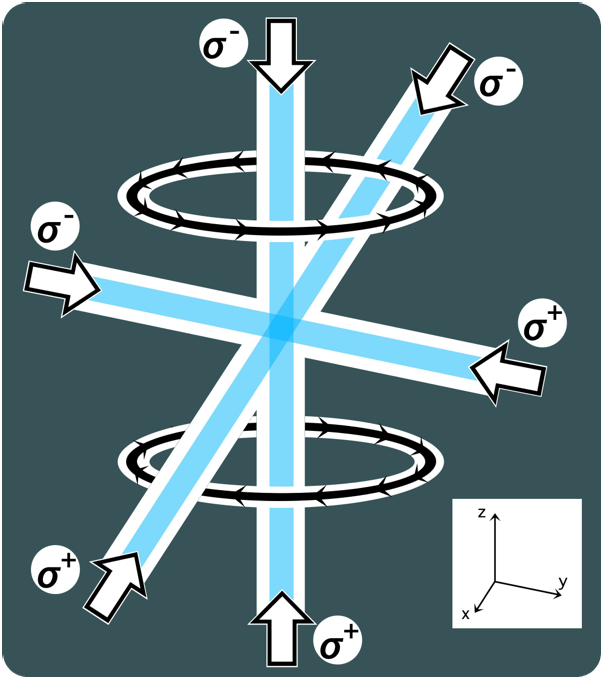
\includegraphics[width=.237\linewidth]{Figures/mot.png}\label{fig:mot} }
%	\hspace*{\fill}
%%	\hfill
%	\hspace*{\fill}
%	\subfloat[One cycle of trapping with the AC-MOT, followed by optical pumping to spin-polarize the atoms.  After atoms are transferred into the science chamber, this cycle is repeated 500 times before the next transfer.  The magnetic dipole field is created by running parallel (rather than anti-parallel as is needed for the MOT) currents through the two coils.]	
%	{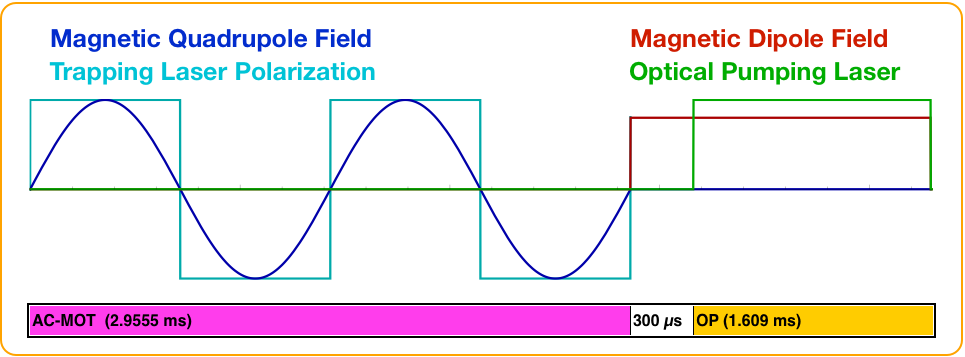
\includegraphics[width=.726\linewidth]{Figures/acmot.png}\label{fig:acmot} }
%	\caption{An alternating-current magneto-optical trap with a duty cycle optimized for producing polarized atoms}	
%	\label{fig:themot}
%\end{figure}
%
%The need to use an AC-MOT rather than a typical MOT has arisen as a direct result of our desire to optimally polarize our sample of atoms.  Polarization is incompatible with the non-uniform magnetic field used by a MOT, and rapidly shutting off the current used to produce the MOT's magnetic field produces eddy currents in the surrounding materials, which in turn produce their own non-uniform magnetic field in the region of interest.  The AC-MOT is developed as a way to ensure that the unavoidable eddy currents are behaving as we expect.  With an appropriate choice of shut-off phase, the current in the coils can be shut off when the overall magnetic field is already zero, so that no further eddy currents are induced.   
%

%
%In order to optimally polarize a sample of atoms by this method, it is necessary to have precise control over the magnetic field.  This is because absent other forces, a spin will undergo Larmor precession about the magnetic field lines.  In particular, the magnetic field must be aligned along the polarization axis (otherwise the tendency will be to actually depolarize the atoms), and it must be uniform in magnitude over the region of interest (otherwise its divergencelessness will result in the field also having a non-uniform direction, which results in a spatially-dependent depolarization mechanism).  Note that this type of magnetic field is not compatible with the MOT, which requires a quadrupolar magnetic field \emph{gradient}, and has necessitated our use of the AC-MOT as described in Subsection~\ref{trap}.

%
%In order to make best use of these MCPs, we create an electric field in order to draw positively charged particles into one MCP, while drawing negatively charged electrons into the other MCP.  Seven electrostatic hoops have been placed within the chamber (see Figure~\ref{fig:thechamber}), and are connected to a series of high voltage power supplies.  See Sections~\ref{photoions} and~\ref{pos_recoils} for a discussion of what sort of charged particles we expect to observe in these detectors and how they are created.  
%  

%Scientific data has been collected at field strengths of 395 V/cm, 415 V/cm, and 535 V/cm.  It should be noted that these field strengths are too low to significantly perturb any but the least energetic of the (positively charged) betas from the decay process, and these low energy betas would already have been unable to reach the upper and lower beta detectors due to interactions with materials in the SiC mirror and Be foil vacuum seal.  
%

%\note[done, nolist]{John says the whole $R_{\textrm{slow}}$ thing should go in here somewhere.}
%\note[done, nolist]{Appendix I  keep, it's excellent. It should be moved as is to Conclusions under "Future Experiment for the collaboration"! so people know you worked so hard on it!!}



\note[done, nolist]{More thoughts from John:
\\...\\
hi Melissa,
\\...\\
I think you should keep Section 6.2, but I think it would be clearer to point out the observable manifests as a dip in the raw TOF spectrum, not going all the way to zero as in the ideal on-axis situation you describe for simplicity.
I.e., I would say you need to qualify this "exactly" word (emphasis mine below), and since
it ends up as a cos(theta) distribution like in my attached slide on the subject, your figure of the TOF spectrum would be a good way to do that.
\\...\\
"Henceforth, daughter nuclei from a back-to-back decay as shown in
Figure ?? will be described as ‘slow’ recoils. In terms of observables, this means that
if the electric field is configured to point along one of the axes perpendicular to the
polarization direction, then when the recoiling ion is swept away into a detector, the
slow recoil’s hit position should be \textbf{exactly}​​ along the projection of the polarization
axis. Furthermore, the slow recoil’s time of flight should be in the middle of the time
of flight spectrum, since other recoils will be emitted with momentum towards or
away from the detector"
}

%%\ifthenelse{\boolean{isdraft}}
%%{
%%\begin{figure}[htb]
%%	\centering
%%	\includegraphics[width=.999\linewidth]{Feedback/AMirrorDecayObservable.png}
%%	\caption[A Slide From John]{A Slide From John, or something.  idk, it goes with the text immediately previous.}
%%%	\label{}
%%\end{figure}
%%\FloatBarrier
%%}
%%{}


%Of course, in any real experiment, the number of decays emitted in exactly one set of directions will be a set of measure zero.  \comment{(say something about the limits taken as beta decay events approach the optimal set of angles.  Or just delete this paragraph because it's stupid.)}
% % %

%\section{Proposed Project}
%\label{project}
%Using $^{37}\textrm{K}$ beta decay data collected in June 2014, I intend to reconstruct the recoil momenta both along the polarization axis and perpendicular to it, such that when combined with energy and hit position from the beta detectors, each event's full kinematics may be reconstructed.  The spectra created by these events will be compared against a series of Geant4-based Monte Carlo simulations.  
%
%Matched template fitting will be used to compare the experimental data to the simulation, meaning that the implicit vector, axial, scalar, and tensor couplings within Eq.~\ref{jtw_pdf} will be allowed to float separately within the simulation, and a series of simulation ``templates'' will be produced, and each separately fit to the data.  The quality of each fit will be used to determine a ``best'' experimental value for both parameters, as well as the error inherent in the measurement.  
%
%%{\color{cyan} (...) }
%%\comment{See Figure~\ref{fig:Rslow_tof} ?}
%\begin{figure}[h!!t]
%	\centering
%	\includegraphics[width=.999\linewidth]
%	{Figures/Rslow_tof_squished.png}
%	\caption{Time-of-flight spectra for charged $^{37}\textrm{\!Ar}$ recoils at 535 V/cm, sorted by whether the $\beta$ was detected after emerging \emph{with} or \emph{against} the nuclear polarization direction, compared against a simulation using a uniform electric field.  	Recoils with zero initial momentum along the flight axis arrive in the center of the distribution for their charge state.  
%	}	
%	\label{fig:Rslow_tof}
%\end{figure}

%%%%
%%%\subsection{Status of the $R_{\textrm{slow}}$ Measurement}
%%%\label{rslow_status}
%%%In June 2014, after several years of preparatory work beforehand (the author has been continuously involved with this project since 2010), approximately 7 days of beam time at TRIUMF was dedicated to the TRINAT $^{37}\textrm{K}$ beta decay experiment.  Approximately half of this data is suitable for use in this project.  During this period, approximately 10,000 atoms were held within the trap at any given time.  The cleaned spectra show around 50,000 polarized beta-recoil coincidence events in total, divided among measurements at three different electric field strengths (535 V/cm, 415 V/cm, 395 V/cm). 
%%%
%%%%At the present time, analysis is underway.  The recoil MCP hit position data has been calibrated, and systematic effects in the trap position and size measurements are being considered.  The largest two remaining hurdles for the analysis both lie in improvements to the Monte Carlo.  
%%%
%%%%The first challenge is to implement particle tracking within a \emph{non-uniform} electric field.  Using the true non-uniform electric field will shift the time-of-flight spectra overall by around 1\%, and is expected to change the \emph{shape} of spectra as well, since the deviation from uniformity changes significantly as a function of flight tragectory, and is greater the farther a particle ventures from the central axis.  This would affect the measured hit positions as well.  Taken together, the shape of the time-of-flight spectra (as in Figure~\ref{fig:Rslow_tof}) and the recoil hit position are critical to our reconstruction of the decay process, it is critical that we model them correctly.  
%%%
%%%%The second challenge will be to allow our simulation to vary vector, axial, scalar, and tensor coupling constants separately while holding other physical parameters (such as the half-life and Fermi/Gamow-Teller ratio) constant.  This, too, will be absolutely critical to the analysis, and its implementation is likely to be non-trivial.
%%%
%%%A fit to simulation has shown that the data that has already been collected has sufficient statistical power to measure the \emph{fractional} contribution of any polarized `new physics' beta decay parameter (ie right-handed, scalar, and tensor currents within the weak interaction) to a sensitivity of $\sim 2\%$ of its true value.  Systematic limitations are still being assessed.  
%%%%Because previous measurements have already shown that any $(V-A)$, $S$, and $T$ terms within the Standard Model must be quite small~\cite{severijns_beck_cuncic_2006}\cite{severijns_cuncic_2011}, the present measurement is not likely to be able to add any new constraints to our understanding of Standard Model physics, and must instead be understood as complementary to previous measurements.
%%%%Because previous measurements have 
%%%%Quantifying this observable's sensitivity to physics beyond the Standard Model in comparison to previously measured constraints~\cite{severijns_beck_cuncic_2006}\cite{severijns_cuncic_2011} is work in progress.  
%%%
%%%
%%%
%%%%Approximately of beamtime and several years of preparatory work beforehand, and its analysis is currently underway.  The statistical strength of our data is sufficient for a \comment{5\%?  (John said 5\%, but I don't really know how he calculated that...)} measurement to constrain right-handed weak interactions, however the systematic effects within the data have not yet been fully evaluated.  This constraint is far too weak to allo w for the discovery of a right-handed component of the nuclear weak force, and is likely also too weak to place any new constraints on its strength.  It could, at best, lend statistical strength to the constraints on right-handed currents that have already been observed.
%%%%
%%%%Unfortunately, due to beam scheduling and target creation procedures at TRIUMF, and because several components of the TRINAT science chamber have subsequently been removed and disassembled to prepare for future upgrades to the apparatus, it would be extremely difficult to collect any further data in a timely fashion.  
%%%
%%%%\pagebreak
%%%


\note[done,nolist]{JB on Ch. \ref{sec:discussion_corrections_uncertainties} -- `discussion of corrections and uncertainties':
\\...\\
could be as simple as
"The bFierz result in Table 5.1 is dominated by statistical uncertainty.
Largely because of this result,
the collaboration is working to reduce the largest systematics,
using lower-Z materials to reduce backscattering, and changing the silicon
delta-E to a multi-wire proportional chamber with very thin windows.
The collaboration has already implemented very thin pellicle mirrors.
The projected systematic uncertainty could approach 0.01 in a future
experment, which would then likely continue to be limited by statistics."
\\...\\
or all of that could go at the end of Chapter 5.
}

%%%%%\note[jb1]{JB on simple things still missing:  
%%%%%\\
%%%%%In Conclusions:
%%%%%\\...\\
%%%%%Comparing bFierz to theory value of 0,  bFierz is (in)consistent with SM
%%%%%at Z sigma.
%%%%%\\...\\
%%%%%Comparing Abeta  and Abeta(theory) the result is (in)consistent with SM at X\% and Y sigma.
%%%%%}
%%%%%
%%%%%%%%Conclusions go here.
%%%%%




%\section{Stuff from John}
\note[jbn, nolist]{Another Round of Thoughts from John!
\\...\\
Fitting Ben's data (using for the bFierz function my convolution of 1/E with a Clifford tail) as I've shown before, compare what happens if I let Abeta float, or if I then fix Abeta arbitrarily to that floated value.
\\
That's not a well-motivated thing to do on its own, but it's not that much different than using Abeta[Cs$^2$,Ct$^2$] constrained by Ft[Cs$^2$,Ct$^2$] since that's only dependent on squares of small quantities.
\\...\\
So I would expect the ability to extract Cs and Ct from the 37K data to have more
sensitivity if Abeta[Cs$^2$,Ct$^2$] and Ft[Cs$^2$,Ct$^2$] and bFierz[Cs,Ct] are floated together in a 2d fit rather then floating Abeta and bFierz without any theoretical constraints and then considering getting linear combinations of Cs and Ct from the bFierz value.
\\...\\
Note that my simply fixing Abeta lowers bFierz uncertainty by a factor of 3. I expect similar improvement in sensitivity to Cs and Ct.
\\...\\
(Here I'm using Cs as a stand-in for (Cs+Cs')/2 for simplicity)
}
\ifthenelse{\boolean{isdraft}}
{
\begin{figure}[htb]
	\centering
	\includegraphics[width=.999\linewidth]{Feedback/FixAndNot.png}
	\caption[A Fit From John]{A Fit From John, or something.  idk, it goes with the text immediately previous.}
%	\label{}
\end{figure}
\FloatBarrier
}
{}

%%%\note[jb1]{Me:
%%%\\
%%%My value of Abeta with bFierz=0 (which I see now that I haven't *actually* included in the text yet.  That clearly needs to happen.) is consistent with Ben's when you account for the fact that Ben's data is, on average, less polarized than he thought.  I think I mention this somewhere, but I probably need to make it more obvious, and located in the 'Conclusions' chapter.  
%%%\\ ... \\
%%%JB:
%%%\\
%%%thanks. Spot-on in your first paragraph--  you know what to do, you just need to write it down.
%%%}
%\note[jb1]{JB:  Dan and I independently discussed (((Ch.~\ref{results_chapter}))) yesterday, and he has suggestions to
%help. So I will also schedule a meeting with Dan and you to discuss
%(((Ch.~\ref{results_chapter}))) Results and whether the S,T part must be deleted and left to a paper.
%You don't have enough time, and although this should be quite straightforward,
%it is not your critical result and it's the only thing that can go.}
\note[jb1]{JB on simple things still missing:
\\
%The final answers with uncertainties are only stated in the caption of Fig. 5.1.
I would have expected a separate uncertainty for b and Abeta for each data set,
either on each 2D figure in ch. 6, are collected in a table in Ch. 6.
}

%\section{That figure from John}
%In which we talk about and possibly *put* Fig.~\ref{fig:exclusionplotfromjohn}.

\note[done, nolist]{
ii) Similarly, answering how the results fit into the bigger picture is what you wanted to do.
\\...\\
I'm convinced that you don't want to do a full review of all beta decay experiments.
\\...\\
But you could say the Fierz term has been constrained by the energy spectrum and by the energy dependence of the beta
asymmetry, cite the best paper in the neutron and maybe the UCNA one as well, and use that figure I sent (I'm sending the improved version).
\\...\\
It is a good approximation to linearize the situation, i.e. this figure is good for small Cs and Ct. (A similar approach is being used in a letter coming out soon, and 3 referees did not nag them about it.)
}

\note[jbn, nolist]{Immediate follow-up email from John:  
\\...\\
another basic big point. What would it mean if there were nonzero Cs, Ct? 
\\
In the context of the more elegant SM, a theory of quarks and leptons and mathematically consistent interactions, that would imply the existence of at least one extra unknown exchange boson. The mass would not be measured, just its coupling
strenghts to the particles participating in the beta decay.
\\...\\
Maybe background to understand that includes:
\\
If one were to write the SM weak interaction, $C_A$ and $C_V$ and $C_A$ and $C_V g_A$ would all be constants with abs value 1.
The (1+- gamma\_5)'s are projection operators-- in the SM, the W boson only couples to left-handed nu's and right-handed antinu's
\\
('more will be said in the forward-looking Ch. 6.2 about tests of that part.)
\\
So all the known information about Ca and Cv is accounted for.
\\
($g_A = 1.26$ for the neutron... it's not equal to 1 because of strong interactions between the quarks in the neutron.)
}
















































%
%%%% --- * --- %%%%	
\clearpage

